% Technische Universität Dresden
% Fakultät Informatik
% Institut für Software- und Multimediatechnik
% Seniorprofessur für Multimediatechnik
%
% Example document demonstrating the usage of mmthesis.sty
% 2012-10-26 Andreas Rümpel
% 
% ### build hints (% = filename of tex file) ###
% pdflatex: pdflatex %.tex
% biber: biber % (biber is a modern backend for bibtex, http://biblatex-biber.sourceforge.net)
% glossaries and acronyms: makeglossaries %
%
% Das LATEX2e-Sündenregister: ftp://ftp.dante.de/tex-archive/info/l2tabu/german/l2tabu.pdf
% KOMAScript-Guide: ftp://ftp.dante.de/tex-archive/macros/latex/contrib/koma-script/scrguide.påådf
% Einige typographische Grundregeln und ihre Umsetzung in LaTeX: http://www2.informatik.hu-berlin.de/sv/lehre/typographie.pdf

\documentclass[
	headsepline,
	footsepline,
	fontsize=12pt,
	%draft, % use this for finding overfull boxes
	%parskip, % use this for alternative paragraph formatting
	bibliography=totoc
]{scrbook}

\usepackage{mmthesis}
\usepackage{listings}
% \usepackage{showkeys} % used to show labels
\addbibresource{library.bib} % put name of bib file here with extension

%### switches
%\printoutput % make link colors black, leave deactivated for screen output

%### define metadata
\mmtype{Diplomarbeit} %Diplomarbeit|Großer Beleg|Bachelorarbeit|Masterarbeit|Seminararbeit
\mmtitle{Semantik-gestütztes Hilfesystem für ein komposites Informationsvisualisierungssystem}
\mmtshorttitle{Hilfesystem für komposite InfoVis}
\mmtauthor{Nikolaus Piccolotto}
\mmtsubmissionmonth{November 2013}
\mmtsubmissiondate{30. November 2013}
\mmtsupervisor{Dipl.-Medieninf. Martin Voigt}
%\mmtsupervisorii{Dipl.-Medieninf. Foo Bar} % Co-supervisor, optional

\mmthypersetup % has to be called after setting metadata

%### acronyms
\newacronym{PDF}{PDF}{Portable Document Format}
\newacronym{RCP}{RCP}{Rich Client Platform}
\newacronym{RIA}{RIA}{Rich Internet Application}
\newacronym{RELAXNG}{RELAX NG}{Regular Language Description for XML New Generation}
\newacronym{SGML}{SGML}{Standard Generalized Markup Language}
\newacronym{SWT}{SWT}{Standard Widget Toolkit}
\newacronym{WDC}{W3C}{World Wide Web Consortium}
\newacronym{WPF}{WPF}{Windows Presentation Foundation}
\newacronym{XPath}{XPath}{XML Path Language}
\newacronym{XHTML}{XHTML}{Extensible Hypertext Markup Language}
\newacronym{XML}{XML}{Extensible Markup Language}
% my acronyms
\newacronym{InfoVis}{InfoVis}{Informationsvisualisierung}

\begin{document}
\frontmatter
\pagenumbering{Roman}
\mmtfrontmatter

\listoffigures
\listoftables
\printglossary[type=\acronymtype,style=long,title=Abkürzungsverzeichnis,toctitle=Abkürzungsverzeichnis]
%\printglossary %Glossar

\mainmatter

% ###################################################
\chapter{Einleitung}
\label{chapter:einleitung}

% Einleitung - viele semantische Daten, diese sind sehr nützlich

Im Laufe der letzten Jahre wurden immer mehr semantische Daten veröffentlicht, sowohl in Community-Projekten wie der DBpedia\footnote{\url{http://dbpedia.org}} als auch als Teil der Open Data bzw. Open Government Bewegung, wie z.\,B. data.gov.uk\footnote{\url{http://data.gov.uk/data/search?q=rdf}}. Diese Datenkataloge können von großem Nutzen für jeden sein. Die DBpedia ist eine maschinenlesbare Version der Wikipedia, mit ihr können mit Hilfe der Abfragesprache SPARQL automatisch Fragen beantwortet werden, deren manuelle Recherche zu aufwändig wäre. In data.gov.uk finden sich Informationen, die für alle Steuerzahler im Vereinigten Königreich relevant sein können, wie z.\,B. Organigramme und Gehälter von Regierungsorganisationen.

% ###################################################
\section{Motivation}
\label{section:einleitung:motivation}

% Motivation - es gibt keine gute Möglichkeit, das Wissen in den Daten aufzunehmen. 

% expertenwissen informatik

Jedoch ist es sehr schwierig, das Wissen in den Datenkatalogen aufzunehmen. Wird wie im Falle der DBpedia eine API in Form eines SPARQL Endpoints zur Verfügung gestellt, müssen sowohl die Abfragesprache SPARQL als auch Konzepte von semantischen Daten wie z.\,B. Tripel, Klassen oder Vererbung bekannt sein, um an die Daten zu kommen. Erlaubt das Portal einen Download der Daten, stellt sich die Frage, wie sie geöffnet werden. Gängige Datenverarbeitungstools wie Excel oder Visualisierungstools wie Tableau unterstützen keine semantischen Daten. Es existieren zwar Visualisierungstools für semantische Daten wie Protégé/Jambalaya, diese stellen aber oft nur einen Graphen dar. Die Visualisierung als Netzwerk kann wie im Fall von Organigrammen angebracht sein, aber bei Daten über Aktienkurse wäre ein Liniendiagramm vielleicht besser geeignet.

% expertenwissen visualisierung

Selbst wenn ein Visualisierungstool für semantische Daten existierte, welches verschiedene Arten von Diagrammen unterstützt, würde ein Anwender das Wissen in den Datenkatalogen nicht angemessen vermittelt bekommen. Die Konfiguration von Diagrammen setzt Expertenwissen im Bereich der Informationsvisualisierung voraus, die in den meisten Fällen nicht gegeben ist. Wie viele Farben können in einem Diagramm unterschieden werden? Wie viele Balken sind zu viele für ein Balkendiagramm? Welche Informationen werden am Besten als Farbe kodiert, welche als Größe oder Position?

% vizboard to the rescue

Diese Probleme zu lösen ist das Ziel des Forschungsprojekts VizBoard. Es setzt einen Prozess aus fünf Schritten ein (Abbildung~\ref{figure:vizboard_workflow}): Zuerst wird ein Datensatz hochgeladen (1), danach Konzepte zur Visualisierung ausgewählt (3), Daten im Detail und Visualisierungen gewählt (5), Visualisierungen konfiguriert (7) und schließlich werden die Visualisierungen angezeigt (9).

\begin{figure}[htbp]
	\centering
	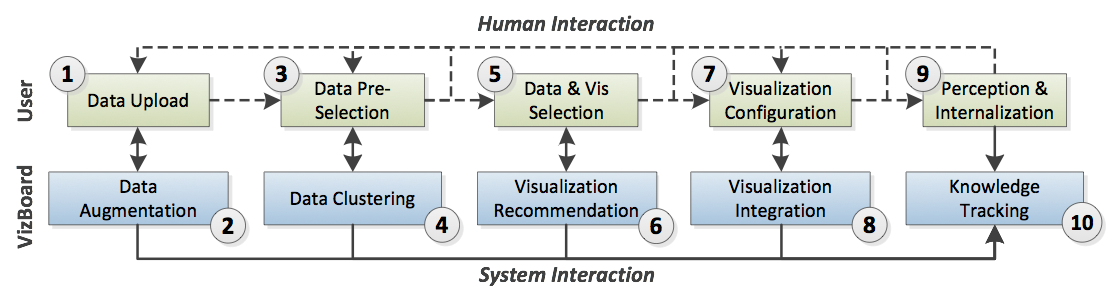
\includegraphics[width=0.75\textwidth]{images/vizboard_workflow.png}
	\caption{VizBoard Workflow}
	\label{figure:vizboard_workflow}
\end{figure}

% ###################################################
\section{Problemstellung und Zielsetzung}
\label{section:einleitung:problemstellung}

% problem liegt im letzten teil

Im letzten Schritt 



% ###################################################
\section{Aufbau der Arbeit}
\label{section:einleitung:aufbau}

% Aufbau der Arbeit erklären, kommt zum Schluss

% ###################################################
\chapter{Stand der Forschung und Technik}
\label{chapter:standderforschung}

Der folgende Abschnitt besteht aus drei Teilen. Zuerst wird die Aufgabenstellung in einem Szenario verdeutlicht (Abschnitt~\ref{section:standderforschung:szenario}). Daraus werden Anforderungen an das Hilfesystem abgeleitet (Abschnitt~\ref{section:standderforschung:anforderungsanalyse}) und danach die Grundlagen von semantischen Daten, Informationsvisualisierungen und Software Support erläutert (Abschnitt~\ref{section:standderforschung:grundlagen}).

% ###################################################
\section{Szenario}
\label{section:standderforschung:szenario}

% kurze einleitung noch mal

Wie in Kapitel~\ref{chapter:einleitung} erläutert, ist das komposite InfoVis-System Teil der webbasierten Anwendung VizBoard. Sie leitet den Benutzer in mehreren Schritten von der Auswahl eines Datensatzes zur finalen, kompositen Informationsvisualisierung. Im vorletzten Schritt wählt dieser mit Hilfe eines Facettenbrowsers geeignete Visualisierungskomponenten aus, welche danach angezeigt werden. Um die Problemstellung noch einmal zu verdeutlichen, wird im folgenden ein mögliches Szenario beschrieben.

% einführung der problemstellung
Anna möchte für ihr Biologiestudium mehr über die geografische Verteilung verschiedener Genvarationen herausfinden. Dazu sucht sie im Internet nach einem Datensatz, welchen sie auch findet. 
% unbekanntes format, kann es nirgends ordentlich öffen und selbst wenn es in excel ginge, wüsste sie nicht, welche charts sie am besten erstellen sollte
Leider ist er in einem für Anna unbekannten Format abgespeichert, nämlich OWL. Sie versucht die Datei mit Microsoft Excel und SPSS zu öffnen, weil sie keine anderen Programme zur Datenverarbeitung kennt, aber scheitert. Anna stellt fest, dass nur ihr Texteditor OWL öffnen und vernünftig darstellen kann. Als sie die Datei überfliegt, kann sie den Inhalt zwar erahnen, aber es ist einfach zu viel Text um ihn vollständig zu lesen. Davon abgesehen sind geografische Breite und Länge als Zahlenkombination keine anschauliche Repräsentation von Orten, auch Verteilungen von Werten sind so schwer ersichtlich. Anna würde viel Zeit aufwenden müssen um sehr wenig des Inhalts zu verstehen. Aber selbst wenn sie die Datei in Excel hätte öffnen können, hätte sie nicht gewusst, mit welchen Diagrammen die vorhandenen Daten am Besten verstanden würden. Anna hört von einem Freund, dass VizBoard gut geeignet ist, um semantische Datensätze anzusehen und probiert es aus.

% Der Benutzer ist laut unserem Rollenmodell weder Developer noch Visualisierungsexperte, d.h. er hat erstmal Schwierigkeiten zu erfassen, was hier überhaupt abgeht

Anna hat ihren Datensatz auch bei VizBoard gefunden und ist neugierig: Sie wählt eine Karte, ein Balkendiagramm, eine Tabelle und eine Treemap aus (Abbildung~\ref{figure:szenario-skizze}); kurz darauf werden ihr die Visualisierungskomponenten angezeigt. Anna benutzt VizBoard zum ersten Mal und macht außer Facebook und YouTube auch sonst nicht viel im Internet, das heißt sie ist zunächst von den vier unterschiedlichen Fenstern etwas überfordert.

\begin{figure}[htbp]
	\centering
	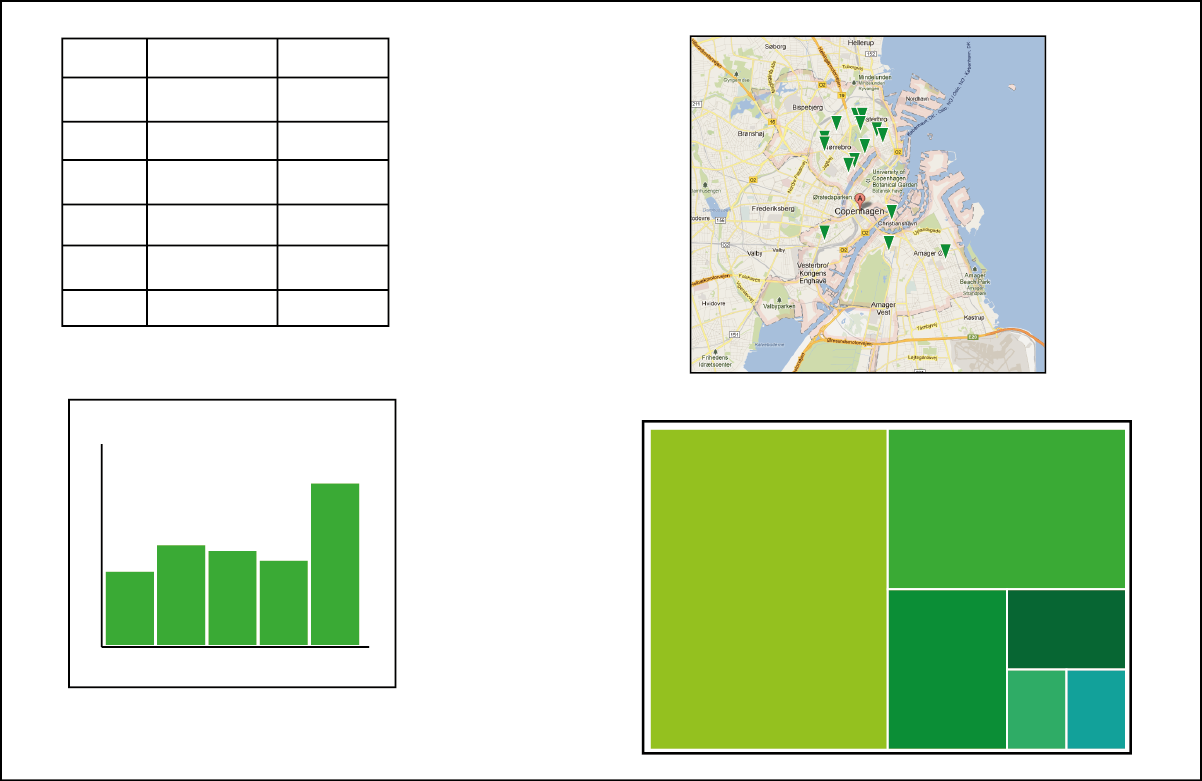
\includegraphics[width=0.75\textwidth]{images/szenario-skizze.png}
	\caption{Skizze der VizBoard Visualisierungskomponenten}
	\label{figure:szenario-skizze}
\end{figure}

VizBoard bietet Anna aber sofort eine einführende Übersicht und erklärt kurz die Darstellungsform und den Inhalt jeder Komponente. Eine denkbare Erklärung der Treemap wäre zum Beispiel:

\begin{quote}
Eine Treemap ist eine hierarchische Visualisierung, um Größenverhältnisse anschaulich zu machen. In dieser werden die Anzahl von Genvariationen pro geografischer Region dargestellt.
\end{quote}

% Was sind das für Fenster? Welche Komponente ist welche? Welche macht was? Wie kann ich sie bedienen? HUUUPS da ändert sich ja was obwohl ich dort nix gemacht hab! Wie hängen die zusammen? Was sind das für Daten, die dargestellt werden? 

Damit bekommt Anna einen Überblick über die verfügbaren Visualisierungen und weiß, welches Fenster welche Visualisierung enthält und für was diese gut sind. Nun möchte sie die Tabelle, in der die durch die Treemap visualisierten Daten stehen, nach der Spalte \enquote{Anzahl} sortieren. Anna sieht aber nicht, wie sie das machen soll, da in der Tabelle kein offensichtliches Kontrollelement wie z.\,B. ein Button vorhanden ist. Sie bemerkt ein Fragezeichen in der Titelleiste des Fensters und klickt darauf. Der verfügbare Viewport wird abgedunkelt und es erscheint ein neues Fenster, welches die verfügbaren Aktionen mit Hilfe von Text, Bildern und Animationen erklärt. Anna lernt, dass sie mit einem einfachen Linksklick auf den jeweiligen Kopf einer Tabellenspalte nach dieser sortieren kann und außerdem eine oder mehrere Zeilen auswählen kann. Sie sortiert die Tabelle wie gewollt und wählt die ersten drei Zeilen aus. Plötzlich verkleinert die Karte ihr Zoomlevel und Anna ist verwirrt: Sie hat nur mit der Tabelle interagiert und es bestand keine sichtbare Verbindung zwischen den beiden Fenstern. Allerdings wurde nach der Zeilenauswahl ein Pfeil von der Tabelle zur Karte gezeichnet, welcher mit einem Icon in Form eines Briefes versehen ist. Anna vermutet, dass doch irgendeine Verbindung zwischen den beiden Visualisierungen besteht und klickt auf den Brief. Ähnlich wie vorhin bei der Hilfe zur Tabelle wird der Viewport abgedunkelt und ein neues Fenster wird eingeblendet. Es erklärt die Kommunikation zwischen den Visualisierungen mit Hilfe von Animationen, Text und Bildern. Nun weiß Anna auch, wie die verschiedenen Fenster zusammenhängen und kann sich ihrer eigentlichen Aufgabe widmen.

% Was heißt GDP? Wie wird das berechnet? Was soll die Spitze bei 1990? Woher kommt die? Diese eine Komponente scheint kaputt zu sein, wo kann ich mich beschweren?

In der Tabelle findet sie auch eine Spalte \enquote{SNP}. Anna weiß zwar, dass sie die Abkürzung schon einmal gesehen hat, kennt aber im Moment ihre Bedeutung nicht. Praktischerweise ist der Spaltenkopf mit der Wikipedia verlinkt und sie wird sofort auf die entsprechende Seite weitergeleitet. Anna erinnert sich, dass \enquote{SNP} \enquote{Single-nucleotide polymorphism} bedeutet und sie bekommt auch gleich zusätzliche Informationen zu diesem Thema. Sie widmet sich weiter der Tabelle und stellt fest, dass die Ortsbezeichnung \enquote{Kopenhagen} nicht mit der Markierung in der Karte übereinstimmt. Außerdem ist sie erstaunt, wie hoch die Verbreitung eines bestimmten SNPs dort ist und würde gerne die Ursache dafür wissen. In der Hilfe zur Tabelle wurde sie auch über die Möglichkeit, Kommentare an den Daten vorzunehmen, aufgeklärt. Anna kommentiert sowohl die falschen Geokoordinaten als auch ihre Frage über die Verbreitung des SNPs, sodass sie später über Antworten informiert wird. Nun kann Anna sich mit der vierten Visualisierung, dem Balkendiagramm, beschäftigen. Allerdings reagiert es auf keine Mausklicks und macht auch sonst nicht den Eindruck, die Daten akkurat darzustellen. Anna meldet die kaputte Visualisierung über die eingebaute Reporting-Funktion und schließt das Fenster, um sich den anderen drei Visualisierungskomponenten zuzuwenden.

% ###################################################
\section{Anforderungsanalyse}
\label{section:standderforschung:anforderungsanalyse}

Aus dem Szenario (Kapitel~\ref{section:standderforschung:szenario}) lassen sich nun verschiedene Anforderungen an ein Hilfesystem für komposite Informationsvisualisierungssysteme ableiten.

\subsection{Funktionale Anforderungen}
\label{section:standderforschung:anforderungsanalyse:funktionale_anforderungen}

Blabla

\begin{itemize}
	\item\textbf{Intro}: Das Hilfesystem soll einen kurzen Überblick über das InfoVis-System geben und Darstellungsform sowie Inhalt jeder Komponente kurz erläutern.
	\item\textbf{Bedienung}: Das Hilfesystem soll erklären können, wie eine Komponente bedient wird. Diese Informationen umfassen beispielsweise welche Operationen welche Aktionen (eventuell auf welchen Daten) ausführen.
	\item\textbf{Reporting}: Fehler in Komponenten sollen über ein Reporting-System gemeldet werden können.
	\item\textbf{Verlinkung}: Das Hilfesystem soll nicht-triviale Begriffe mit einer Wissensbasis‚ verlinken, sodass nicht nur auf die Begriffsbedeutung hingewiesen werden, sondern dem Benutzer auch zusätzliche Informationen zur Verfügung gestellt werden können.
	\item\textbf{Kommunikation}: Das Hilfesystem soll erklären können, wie gegebene Komponenten miteinander kommunizieren.
	\item\textbf{Kommentare}: Der Benutzer soll die Möglichkeit haben Daten zu kommentieren und Bereiche der Visualisierung zu markieren und mit ebenfalls mit einem Kommentar zu versehen, sodass auch auf fehlende Daten hingewiesen werden kann.
\end{itemize}

% was muss also ins related work?
% wie der wissensaufnahmeprozess funktioniert, weil ich ja erklärungen gebe, speziell planerklärung
% was es so für infovis gibt, weil ich mit denen arbeite
% was es so für hilfekonzepte gibt, weil es das ist was ich tue
% social web, weil kommentare implementiert werden

\subsection{Nichtfunktionale Anforderungen}
\label{section:standderforschung:anforderungsanalyse:nichtfunktionale_anforderungen}

Bla bla

\begin{itemize}
	\item\textbf{Korrektheit}: Eine gegebene Hilfestellung darf keine Fehlinformationen enthalten, weil sie sonst mehr verwirrt als hilft.
	\item\textbf{Vollständigkeit}: Eine gegebene Hilfestellung muss alle Informationen enthalten, die der Nutzer benötigt um danach seine gewünschte Aufgabe ausführen zu können.
	\item\textbf{Verständlichkeit}: Hilfestellungen müssen in einer Form präsentiert werden, die der Benutzer schnell und mit geringem mentalen Aufwand verarbeiten kann.
	\item\textbf{Einheitlichkeit}: Das Look \& Feel von Teilen des Hilfesystems (z.B. Kommentare) muss komponentenübergreifend einheitlich sein, damit der Benutzer einmal gelerntes wiederverwenden kann.
	\item\textbf{Minimalität}: Der Komponentenentwickler soll seine Komponente mit möglichst wenig Aufwand zum Hilfesystem kompatibel machen können, ansonsten werden nur sehr wenige Komponenten -- und damit der Benutzer -- davon profitieren.
	\item\textbf{Universalität}: Das Hilfesystem soll für alle Komponenten und Visualisierungen in gleicher Qualität funktionieren.
	\item\textbf{Wiederverwendbarkeit}: Die Kommentare sollen möglichst in allen Visualisierungen wiederverwendet werden, damit viele Benutzer von den Erkenntnissen anderer profitieren können.
	\item\textbf{Unaufdringlichkeit}: Das Hilfesystem soll den Benutzer nicht von seinen Aufgaben ablenken und nur auf Anfrage zum Einsatz kommen oder es soll selbständig erkennen, wenn der Benutzer Hilfe benötigt.
\end{itemize}

% ###################################################
\section{Grundlagen}
\label{section:standderforschung:grundlagen}

Hurrrrr derp herp

\subsection{CRUISe, EDYRA \& VizBoard}
\label{section:standderforschung:grundlagen:cruise_vizboard}

% grundlagen von cruise edyra vizboard. wichtig weil mein hilfesystem dort eingesetzt wird
CRUISe \cite{Pietschmann2009, Pietschmann2012} ist ein Framework zur Konstruktion von webbasierten, kompositen User Interfaces (auch Mashups). Diese bestehen aus mehreren voneinander unabhängigen, wiederverwendbaren User Interface Services (z.\,B. eine Karte, eine Tabelle und ein Kalender) welche zur Laufzeit hinzugefügt, konfiguriert und ausgetauscht werden können. Abbildung~\ref{figure:cruise_architektur} zeigt die Architektur von CRUISe. Zuerst werden Komponenten von Entwicklern erstellt und modelliert (1). Danach interpretiert CRUISe das Kompositionsmodell (2), matcht es gegen die Kontextanforderungen (3), bildet ein Ranking (4) und integriert schließlich die am besten geeignete Komponente ins User Interface (5).

\begin{figure}[htbp]
	\centering
	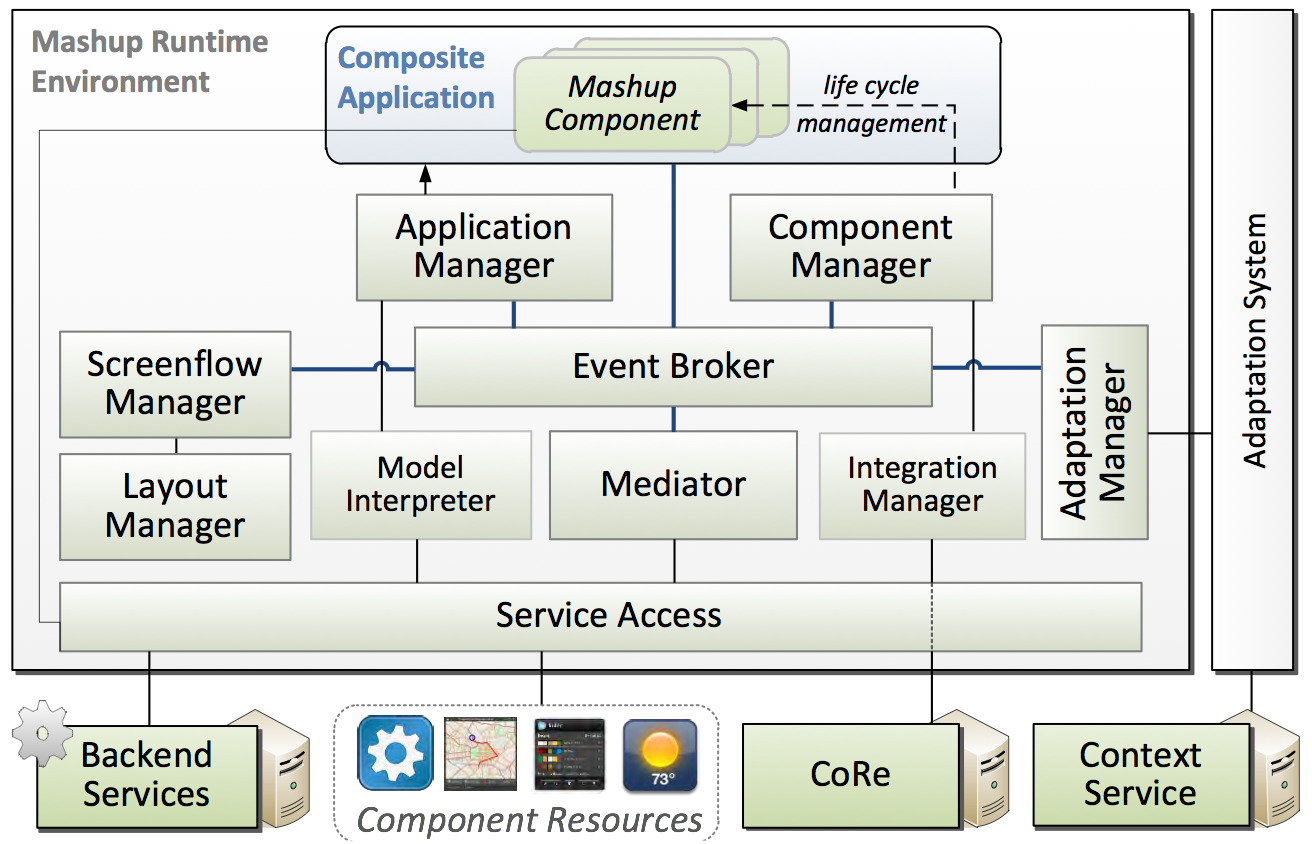
\includegraphics[width=0.75\textwidth]{images/grundlagen-cruise_architektur.png}
	\caption{CRUISe Architektur aus \cite{Pietschmann2012}}
	\label{figure:cruise_architektur}
\end{figure}

CRUISe geht davon aus, dass professionelle Softwarentwickler Komponenten zu kompositen Sichten modellieren, welche dann von Endnutzern nur noch aufgerufen werden. EDYRA \cite{Ruempel2011} greift auf das CRUISe Framework zurück, um es Endnutzern selbst zu ermöglichen, diese Aufgabe auszuführen. Dazu schlägt EDYRA zur Laufzeit Komponenten vor, welche sofort integriert oder gelöscht werden können.

VizBoard \cite{Voigt2013} benutzt das CRUISe Framework, um Endnutzern die Möglichkeit zu geben, semantische Datensätze mit Hilfe verschiedener InfoVis verstehen zu können. Abbildung~\ref{figure:vizboard_architektur} zeigt die Architektur von VizBoard. Die Daten werden zuerst aus verschiedenen Quellen in eine semantische Repräsentation konvertiert und im Data Repository (DaRe, 1) gespeichert. Das Component Repository (CoRe, 3) verwaltet die verschiedenen Visualisierungskomponenten (2) und ist für Matching und Ranking von Komponenten zuständig, bevor sie in der Runtime (4) integriert werden. Sowohl das DaRe als auch das CoRe greifen auf die Visualization Ontology (VISO, 5) zurück, die Wissen über verschiedene Aspekte von Visualisierungen, wie z.\,B. Struktur der visualisierten Daten, Mapping der Daten auf visuelle Attribute oder Interaktionsmöglichkeiten, enthält \cite{Polowinski2013}.
% architekturbild --> vizboard paper

\begin{figure}[htbp]
	\centering
	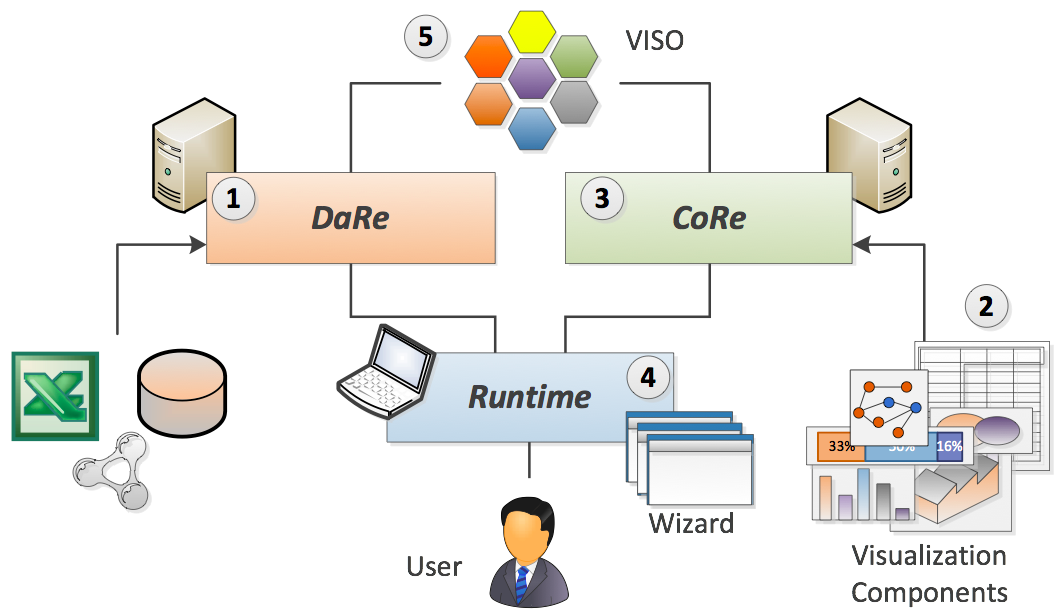
\includegraphics[width=0.75\textwidth]{images/grundlagen-vizboard_architektur.png}
	\caption{VizBoard Architektur aus \cite{Voigt2013}}
	\label{figure:vizboard_architektur}
\end{figure}

\subsubsection{Data Repository}
\label{section:standderforschung_data_repository}

% dare --> vizboard paper, beleg
Im DaRe werden Daten aus verschiedenen Quellen in einer semantischen Repräsentation gespeichert. Dabei durchläuft das DaRe verschiedene Phasen (Abbildung~\ref{figure:dare_phasen}). Zuerst wird der Datensatz \emph{analysiert} und Metainformationen gesammelt, beispielsweise werden Subklassen gezählt und wichtige Konzepte identifiziert. Diese werden an den Datensatz \emph{annotiert}. Zur Laufzeit müssen diese Erkenntnisse wieder aus dem Datensatz \emph{extrahiert} werden. Das DaRe stellt eine REST API zur Verfügung, über die ein Datensatz abgerufen werden kann \cite{Piccolotto2012}.

\subsubsection{Komponentenbeschreibung}
\label{section:standderforschung:grundlagen:cruise_vizboard:komponentenbeschreibung}

% komponentenbeschreibung 5.1.3
Komponenten in CRUISe werden generisch und einheitlich durch Properties, Events und Operationen sowie Metainformationen beschrieben. Properties geben Auskunft über den Zustand einer Komponente, also beispielsweise Breite und Höhe oder die Sortierreihenfolge der Elemente. Events weisen andere Komponenten auf interne Zustandsänderungen hin, zum Beispiel wenn sich die Sortierreihenfolge geändert hat. Operationen sind Methoden einer Komponente, die durch Events ausgelöst werden, z.\,B. \texttt{reassignNumbers(order)}, um die Nummerierung der Pins in einer Karte anzupassen. Zu den Metainformationen gehören u.\,a. der Name einer Komponente oder der Preis.

\subsubsection{Kommunikationsmodell}
\label{section:standderforschung:grundlagen:cruise_vizboard:kommunikationsmodell}

% kommunikationsmodell 5.2.2
Die Kommunikation von Komponenten untereinander ist ereignisgesteuert, d.\,h. eine Komponente veröffentlicht ein Event, dessen Nachricht mit Hilfe des Publish/Subscribe Paradigma an alle Subscriber in diesem Kanal (Link) übertragen wird. Subscriber reagieren auf das Event, indem sie bestimmte Operationen ausführen. Die Übertragung der Nachrichten wird durch sogenannte Links umgesetzt, welche $n$ Events mit $m$ Operationen verbinden. Spezielle Links sind Backlinks, die eine Zweiwegekommunikation zwischen Komponenten ermöglichen und PropertyLinks, die Properties synchron halten. Ein Überblick über die verschiedenen Links ist in Abbildung~\ref{figure:cruise_links} zu sehen.

\begin{figure}[htbp]
	\centering
	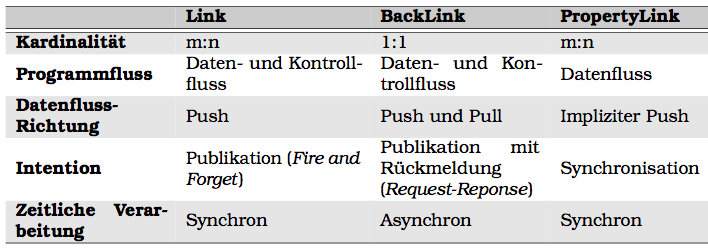
\includegraphics[width=0.75\textwidth]{images/grundlagen-cruise_links.png}
	\caption{CRUISe Links aus \cite{Pietschmann2012}}
	\label{figure:cruise_links}
\end{figure}

\subsubsection{Laufzeitumgebung}
\label{section:standderforschung:grundlagen:cruise_vizboard:laufzeitumgebung}

Die Laufzeitumgebung (Mashup Runtime Environment, MRE) ist für die Ausführung und Verwaltung der kompositen Anwendung verantwortlich und besteht aus mehreren Modulen (Abbildung~\ref{figure:cruise_mre}).

% laufzeitumgebung (tsr) 6.2, 7.2.2
\begin{figure}[htbp]
	\centering
	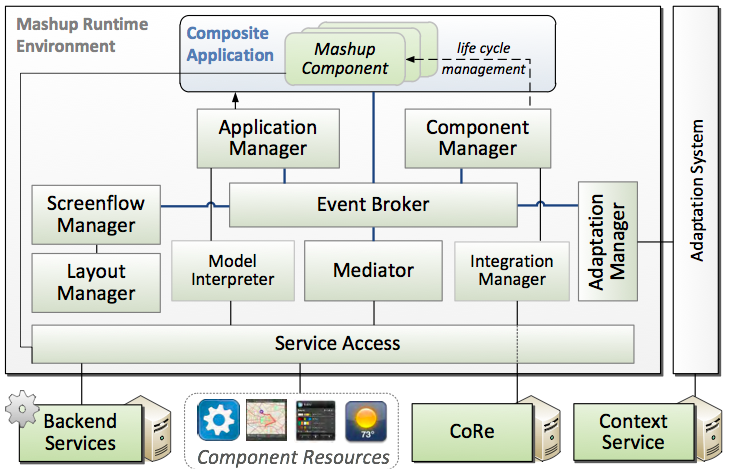
\includegraphics[width=0.75\textwidth]{images/grundlagen-cruise_mre.png}
	\caption{Mashup Runtime Environment Architektur aus \cite{Pietschmann2012}}
	\label{figure:cruise_mre}
\end{figure}

Der \textbf{Application Manager} initialisiert alle anderen Module und ist für die globale Fehlerbehandlung zuständig. Für den Lebenszyklus der einzelnen Komponenten ist der \textbf{Component Manager} zuständig. Die Integration übernimmt allerdings der \textbf{Integration Manager}. Im Mashup Modell definierte Sichten und Übergänge zwischen ihnen werden vom \textbf{Screenflow Manager} interpretiert. Gerendert werden die Komponenten aber vom \textbf{Layout Manager}. Nachrichten zwischen Komponenten der Anwendung und Modulen der MRE werden durch den \textbf{Event Broker} übermittelt. Sind die Parameter von Event und Operation syntaktisch nicht äquivalent, aber semantisch aufeinander abbildbar (z.\,B. zwei gleiche Konzepte aus verschiedenen Namespaces wie \texttt{dbpedia:city} und \texttt{geonames:city}), übernimmt dies der \textbf{Mediator}. Die dynamische Anpassung der Anwendung (z.\,B. von Komponenten, Layout und Kommunikationsmodell) wird gegebenenfalls durch den \textbf{Adaptation Manager} durchgeführt. Der \textbf{Context Service} \cite{Pietschmann2008} speichert Informationen über den Nutzungskontext, beispielsweise den Aufenthaltsort des Nutzers. Letztlich erlaubt das \textbf{Service Access} Modul Zugriff auf Web-Dienste und Ressourcen im Backend.

\subsubsection{VISO}
\label{section:standderforschung:grundlagen:cruise_vizboard:viso}

% viso
In der Visualization Ontology (VISO) ist Visualisierungswissen gespeichert. Sie kann dabei helfen, zur Laufzeit die Domäne dargestellter Daten zu identifizieren oder notwendiges Wissen zur User Assistance (Abschnitt~\ref{section:standderforschung:user_assistance}) zur Komponentenbeschreibung hinzuzufügen. Unter anderem enthält sie folgende Konzepte und deren Verbindungen untereinander:

\begin{itemize}
	\item Visualisierte Daten (\texttt{viso:data})
	\begin{itemize}
		\item Scale of Measurement (nominal, ordinal, quantitativ, unstrukturiert)
		\item Struktur der Daten (tabellarisch, Tripel, verlinkt)
		\item Art der Variable (abhängig, unabhängig, Dimension etc.)
		\item Domäne
	\end{itemize}
	\item Aktivitäten (\texttt{viso:activity})
	\begin{itemize}
		\item Nutzeraktivitäten (Operationen, Aktionen, Aufgaben)
		\item Visualisierungspipeline (Editieren, Visual Mapping, Datentransformation etc.)
	\end{itemize}
	\item Grafikvokabular (\texttt{viso:graphic})
	\begin{itemize}
		\item Visuelle Attribute (Größe, Farbe, Textur etc.)
		\item Koordinaten (kartesisch, Zylinder, Kugel etc.)
		\item Art der grafischen Repräsentation (Karten, Chart mit zwei Achsen, animierte InfoVis etc.)
		\item Beziehungen zwischen Objekten (Clustering, Labeling, verlinkt etc.)
	\end{itemize}
	\item System (\texttt{viso:system})
	\begin{itemize}
		\item Hardware
		\item Software
		\item Bildschirmauflösung
		\item Rundes, eckiges oder unstrukturiertes Display
	\end{itemize}
\end{itemize}

Dieses Wissen wird in VizBoard auf verschiedene Art und Weise genutzt (Abbildung~\ref{figure:viso}). Mit Hilfe der VISO kann Wissen von Visualisierungsexperten formalisiert und im Rankingalgorithmus berücksichtigt werden (2). Gleichermaßen wird sie zur Annotation der Daten im Data Repository (Abschnitt~\ref{section:standderforschung_data_repository}) benutzt (3). Visualisierungskomponenten (4) und Nutzer- bzw. Systemkontext (5) werden durch VISO-Konzepte beschrieben.

\begin{figure}[htbp]
	\centering
	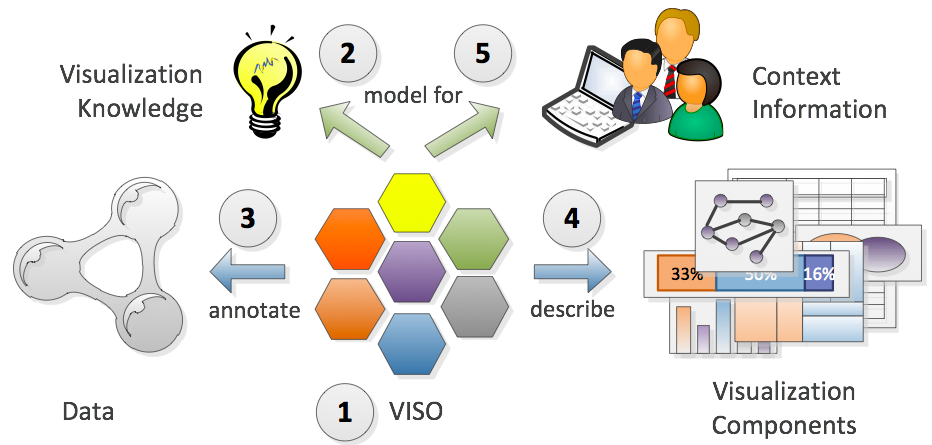
\includegraphics[width=0.75\textwidth]{images/grundlagen-viso.png}
	\caption{Nutzung der VISO in VizBoard}
	\label{figure:viso}
\end{figure}

\subsection{Semantische Datensätze}
\label{section:standderforschung:grundlagen:semantische_daten}

% Grundlagen von RDF, RDFS, OWL. Wichtig weil später Kommentare wieder in einer Ontologie abgelegt werden müssen
Eine Ontologie ist \enquote{an explicit specification of a conceptualization} \cite{Gruber1995} und wird benutzt um domänenspezifisches Wissen abzubilden \cite{Chandrasekaran1999}. Sie besteht aus mehreren Elementen:

\begin{itemize}
	\item Eine Klasse repräsentiert ein Konzept, eine Entität, ein Ding, beispielsweise ein \textit{Smartphone}.
	\item Eine Instanz ist ein konkretes Objekt einer Klasse, zum Beispiel das \textit{iPhone mit der Seriennummer XYZ-ABC}.
	\item Datenattribute beschreiben eine Instanz näher, zum Beispiel die \textit{Seriennummer} oder \textit{Bildschirmgröße} des iPhones.
	\item Objektattribute beschreiben Beziehungen zwischen Klassen und deren Instanzen, beispielsweise eine Person \textit{besitzt} ein Smartphone.
	\item Außerdem existieren noch Axiome, Regeln, Funktionen und Einschränkungen, welche die Logik einer Ontologie beschreiben.
\end{itemize}

Um eine Ontologie maschinenlesbar darzustellen, hat das World Wide Web Consortium (W3C) verschiedene Beschreibungssprachen eingeführt. Die bekanntesten sind Resource Description Framework (RDF), RDF Schema (RDFS) und Web Ontology Language (OWL). Mit diesen Sprachen lässt sich unterschiedlich viel Semantik u.\,a. in Form von Ontologien, Thesauren oder Vokabularen ausdrücken; die Komplexität der Dokumente und damit der Aufwand, sie zu erstellen, verhalten sich aber direkt proportional (siehe Abbildung~\ref{figure:semantic_spectrum}).

\begin{figure}[htbp]
	\centering
	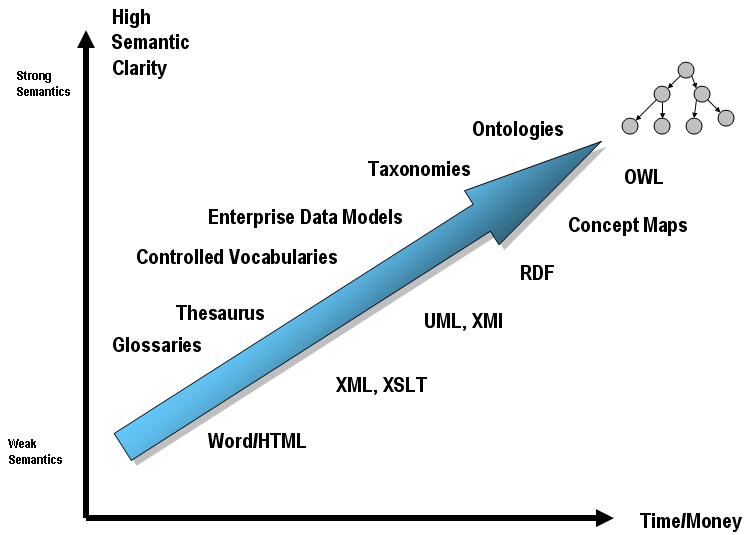
\includegraphics[width=0.75\textwidth]{images/grundlagen-semantic_spectrum.png}
	\caption{Semantic Spectrum \cite{Bergman2007}}
	\label{figure:semantic_spectrum}
\end{figure}

% rdf

RDF ist von den genannten die Sprache mit den wenigsten Features, sie kann nur Tripel der Form (Subjekt, Prädikat, Objekt) darstellen. Die Elemente der Tripel sind Resourcen (durch URIs gekennzeichnet), welche Objekte beschreiben. So drückt der Tripel (\texttt{http://alice.de}, \texttt{http://foaf.de/knows}, \texttt{http://bob.de}) aus, dass das Element \enquote{Alice} mit \enquote{Bob} über die Relation \enquote{knows} verbunden ist. In RDF existieren noch keine Vererbung, Klassen, Properties oder Logik.

% rdfs

RDFS ist eine Erweiterung von RDF, nämlich um Klassen und Vererbung, Datenattribute und Objektattribute. Allerdings ist RDFS damit noch immer nicht so mächtig wie OWL.

% owl

OWL erweitert wiederum RDFS um einige Konzepte. So können beispielsweise Axiome definiert werden, Attribute können als transitiv oder symmetrisch deklariert werden, es existieren Mengenoperationen und Kardinalitäten und Wertebereiche können eingeschränkt werden. OWL existiert in zwei Versionen, da in den meisten Fällen nicht der volle Funktionsumfang benötigt wird: OWL Lite ist für Anwendungen gedacht, die kaum mehr als eine Klassenhierarchie und Attribute benötigen. OWL-DL ist auf die Logik in der Ontologie fokussiert und wird vor allem für Reasoner eingesetzt, um selbstständig Schlüsse innerhalb des vorgegebenen formalen Systems ziehen zu können. OWL 2 wurde 2009 eingeführt, dieser Standard erweitert OWL zum Beispiel um asymmetrische, reflexive und disjunkte Attribute.

\subsection{Informationsvisualisierung}
\label{section:standderforschung:grundlagen:informationsvisualisierung}

% InfoVis Grundlagen. Wichtig weil das die Komponenten sind, mit denen ich zu tun habe.

Card et al. \cite{Card1999} definieren den Begriff \enquote{Informationsvisualisierung} wie folgt:

\begin{quote}
The use of computer-supported, interactive, visual representations of abstract data to amplify cognition.
\end{quote}

Beispiele dafür sind Balkendiagramme, Treemaps \cite{Shneiderman1992} und Parallel Coordinates \cite{Inselberg1991} (Abbildung~\ref{figure:parallel_coordinates}). Mangels Interaktivität sind Infografiken \cite{Smiciklas2012} von den eben definierten Informationsvisualisierungen ausgeschlossen.

\begin{figure}[htbp]
   \centering
   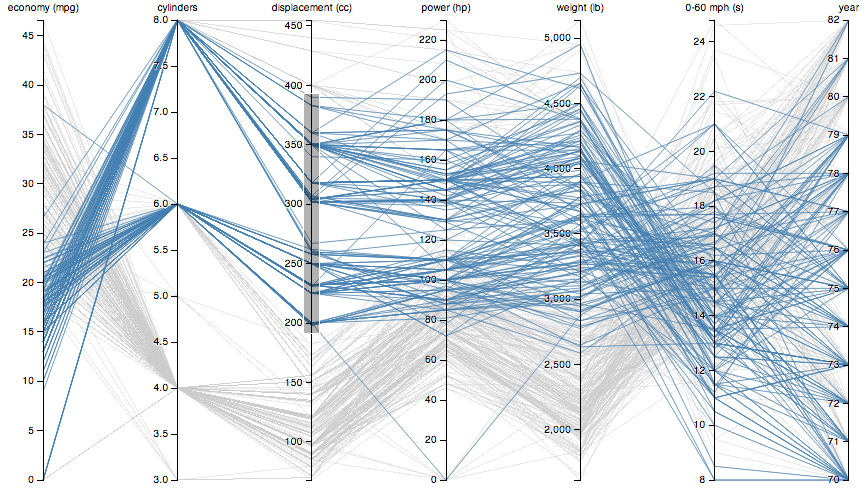
\includegraphics[width=0.5\textwidth]{images/grundlagen-parallel_coordinates.png} 
   \caption{Parallel Coordinates}
   \label{figure:parallel_coordinates}
\end{figure}

% visualisierungsprozess

Informationsvisualisierungen können besonders bei der Exploration großer Datenmengen hilfreich sein \cite{Kohlhammer2011}. Die Wissensaneignung erfolgt dabei iterativ (Abbildung~\ref{figure:visual_analytics_process}). Zuerst werden Daten auf eine Visualisierung gemappt, deren Parameter vom Benutzer geändert werden können. Daraus lernt dieser etwas über die Daten und kann danach (\enquote{Feedback loop}) von vorne anfangen und eine andere Visualisierung wählen oder die Daten transformieren.

\begin{figure}[htbp]
   \centering
   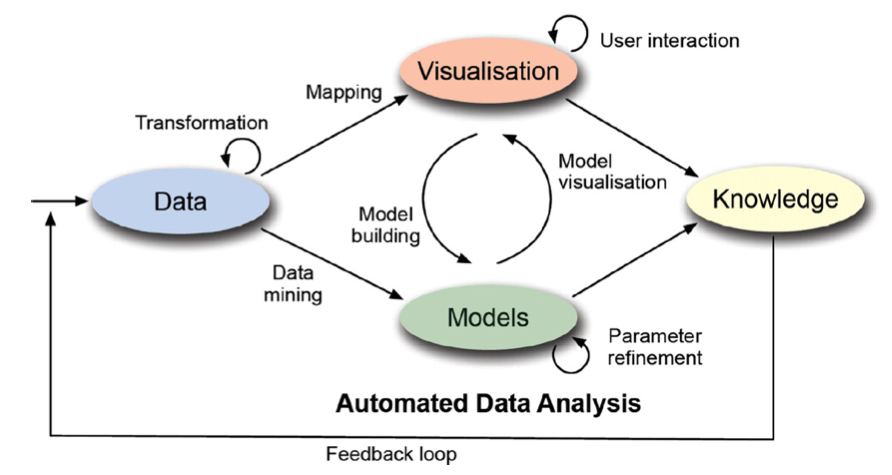
\includegraphics[width=0.5\textwidth]{images/grundlagen-visual_analytics_process.png} 
   \caption{Visual Analytics Process nach \cite{Kohlhammer2011}}
   \label{figure:visual_analytics_process}
\end{figure}

Van Wijk \cite{vanWijk2005} stellt ein ähnliches Modell für den Prozess der Wissensaufnahme über Visualisierungen vor (Abbildung~\ref{figure:visualization_model}). Am Anfang stehen die Daten $D$, welche anhand einer Visualisierungsspezifikation $S$ in eine Visualisierung $V$ transformiert werden. Diese wird vom Benutzer aufgenommen ($P$) und in Wissen ($K$) umgesetzt. Danach startet die Exploration der Daten $E$ indem die Spezifikation geändert und neues Wissen aufgenommen wird (entspricht der \enquote{Feedback loop} aus \cite{Kohlhammer2011}).

\begin{figure}[htbp]
   \centering
   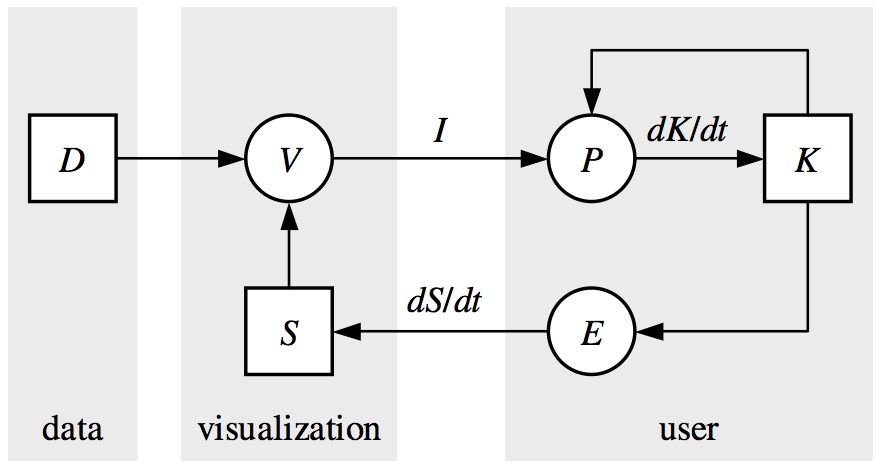
\includegraphics[width=0.5\textwidth]{images/grundlagen-visualization_model.png} 
   \caption{Generic Model on Visualization nach \cite{vanWijk2005}}
   \label{figure:visualization_model}
\end{figure}

% überblick über infovis

Im Folgenden wird ein Überblick über verschiedene Informationsvisualisierungen gegeben. Dieser orientiert sich an Keim \cite{Keim2002}, welcher Informationsvisualisierungen nach dargestellten Daten, Visualisierungs- und Interaktionstechnik klassifizierte. Die Abbildungen stammen, sofern nicht anders angegeben, aus \cite{Heer2010}.

\subsubsection{Dargestellte Daten}
\label{section:standderforschung:grundlagen:informationsvisualisierung:dargestellte_daten}

\textbf{Eindimensionale Daten} sind beispielsweise Zeitreihen, also Folgen von Daten (1992, 1993, 1995...). Nach Keim können diese aber mit anderen Datenobjekten assoziiert sein. Beispiele für InfoVis eindimensionaler Daten wären demnach ein Index Chart (Abbildung~\ref{figure:index_chart}) oder eine einfache Timeline.

\begin{figure}[htbp]
   \centering
   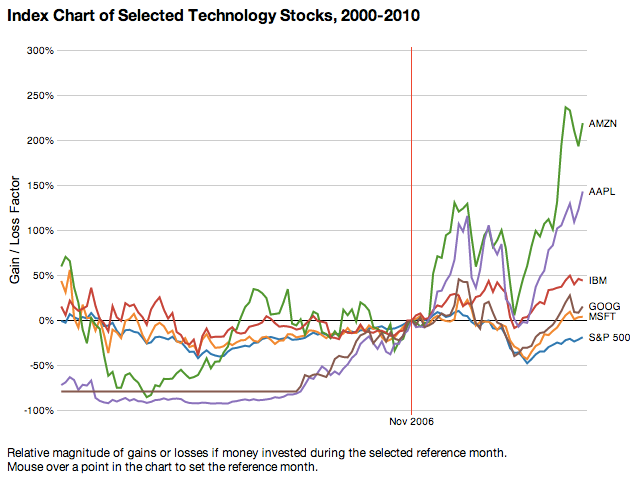
\includegraphics[width=0.5\textwidth]{images/grundlagen-index_chart.png}
   \caption{Index Chart}
   \label{figure:index_chart}
\end{figure}

\textbf{Zweidimensionale Daten} haben zwei unterschiedliche Dimensionen, wie zum Beispiel eine Geokoordinate (geografische Länge und Breite). Beispiele für InfoVis dieser Daten sind eben Karten (Abbildung~\ref{figure:karte}) oder häufig verwendete zweidimensionale Visualisierungen wie z.\,B. ein Balkendiagramm.

\begin{figure}[htbp]
   \centering
   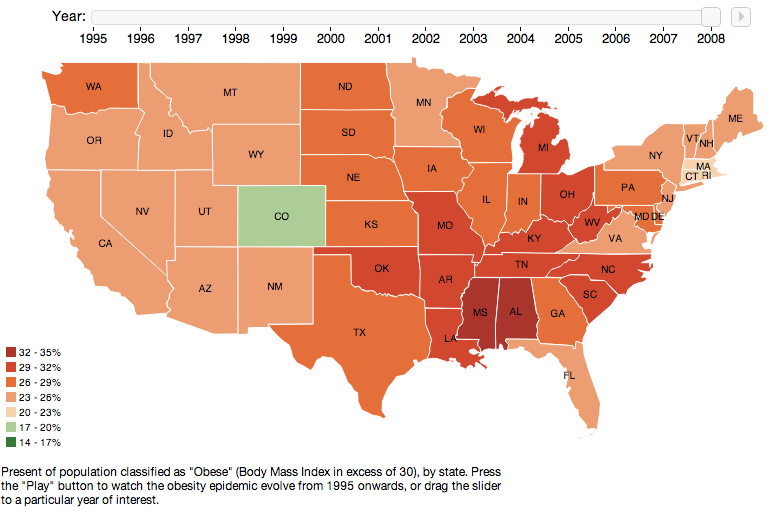
\includegraphics[width=0.5\textwidth]{images/grundlagen-karte.png}
   \caption{Karte}
   \label{figure:karte}
\end{figure}

\textbf{Multidimensionale Daten} haben demnach mehr als zwei unterschiedliche Dimensionen, typischerweise komplexe Objekte wie Autos (Hubraum, Maximalgeschwindigkeit, Leistung, Benzinverbrauch...) oder Digitalkameras (Megapixel, Sensorgröße, maximale Lichtempfindlichkeit, Gewicht...). Um diese Daten darzustellen, werden oft Parallel Coordinates (Abbildung~\ref{figure:parallel_coordinates}) oder Scatterplot Matrizen (Abbildung~\ref{figure:scatterplot_matrix}) verwendet.

\begin{figure}[htbp]
   \centering
   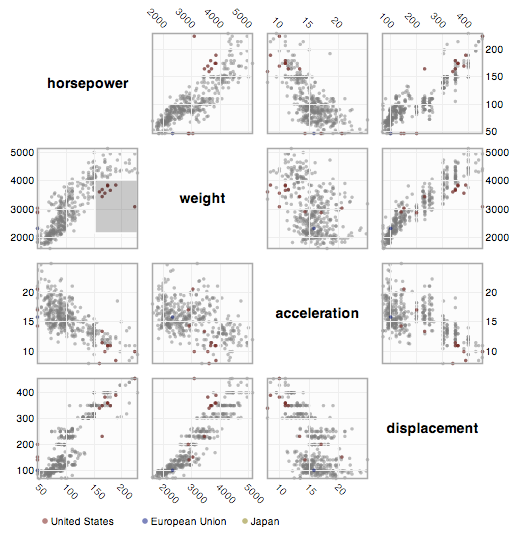
\includegraphics[width=0.5\textwidth]{images/grundlagen-scatterplot_matrix.png}
   \caption{Scatterplot Matrix}
   \label{figure:scatterplot_matrix}
\end{figure}

\textbf{Text} kann erst nach einer Vorverarbeitungsphase mit Zahlen beschrieben werden (z.\,B. Wörter zählen), ansonsten schlagen herkömmliche Visualisierungsansätze fehl. Ein im Web verbreitetes Beispiel ist die Tag Cloud (Abbildung~\ref{figure:tag_cloud}\footnote{\url{http://4.bp.blogspot.com/-WvicpJ9QqQs/TpbqvbKhX3I/AAAAAAAADGc/3PczLY2P0xs/s1600/uni_tag_cloud_wordle.png}}). Je häufiger ein Begriff im Textkorpus vorkommt, desto größer wird er dargestellt.

\begin{figure}[htbp]
   \centering
   
\includegraphics[width=0.5\textwidth]{images/grundlagen-tag_cloud.png}
   \caption{Tag Cloud}
   \label{figure:tag_cloud}
\end{figure}

\textbf{Hierarchien und Netzwerke} beschreiben Relationen und Verbindungen zwischen Objekten. Ein Beispiel für InfoVis von Hierarchien ist der klassische Baum (Abbildung~\ref{figure:baum}), für Netzwerke ein Node-Link-Diagramm (Abbildung~\ref{figure:node-link-diagramm}).

\begin{figure}[htbp]
   \centering
   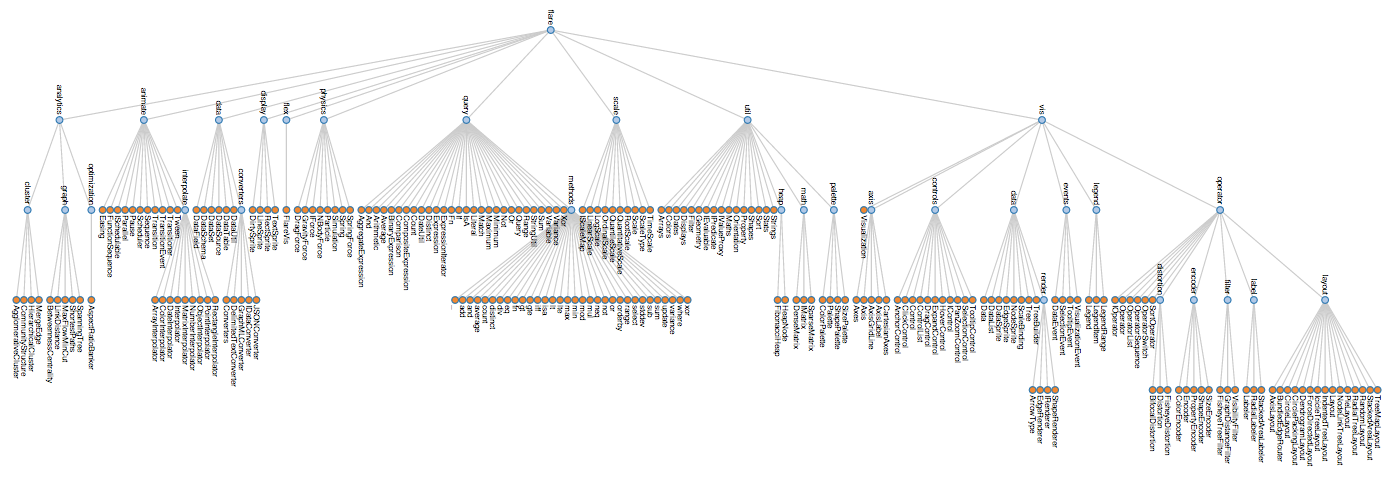
\includegraphics[width=0.75\textwidth]{images/grundlagen-baum.png}
   \caption{Baum}
   \label{figure:baum}
\end{figure}

\begin{figure}[htbp]
   \centering
   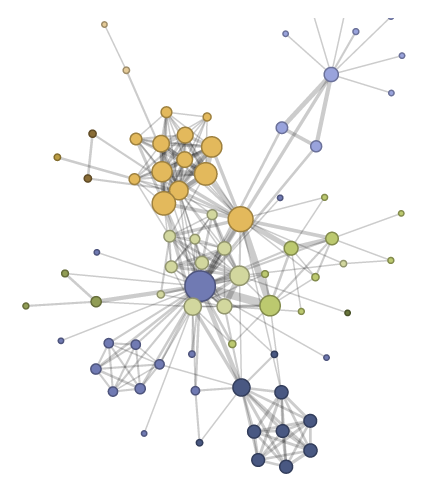
\includegraphics[width=0.25\textwidth]{images/grundlagen-node-link-diagramm.png}
   \caption{Node-Link-Diagramm}
   \label{figure:node-link-diagramm}
\end{figure}

% Am Schluss hat Keim noch Software/Algorithmen, aber ich sehe den Unterschied zu Multidimensionalen Daten nicht. Außerdem kann man - wenn schon mal grundlos neue Kategorien eingeführt werden - dann auch Produktionsprozesse oder what not gesondert betrachten

\subsubsection{Visualisierungstechniken}
\label{section:standderforschung:grundlagen:informationsvisualisierung:visualisierungstechniken}

% standard 2d/3d

\textbf{Standard 2D/3D} Visualisierungen beinhalten Balkendiagramme, Liniendiagramme, sowie andere zweidimensionale Plots und Karten. Ein Beispiel dafür ist das Index Chart (Abbildung~\ref{figure:index_chart}).

% multidimensional
\textbf{Multidimensionale} Visualisierungen\footnote{Die Bezeichnung stammt von Chi \cite{Chi2000} und wird verwendet, da sie logischer erscheint als Keims \enquote{geometrically transformed displays}.} sind Darstellungen multidimensionaler Datensätze jeder Art. Beispiele sind Parallel Coordinates (Abbildung~\ref{figure:parallel_coordinates}) und die Scatterplot Matrix (Abbildung~\ref{figure:scatterplot_matrix}).

% iconic displays

\textbf{Symbolische} Visualisierungen setzen auf verschiedene Art und Weise Symbole ein. Das können auf eine Karte projizierte Kuchendiagramme sein (Abbildung~\ref{figure:symbol_map}) oder Smileys, die abhängig von den Daten lächeln oder weinen \cite{Chernoff1973}.

\begin{figure}[htbp]
   \centering
   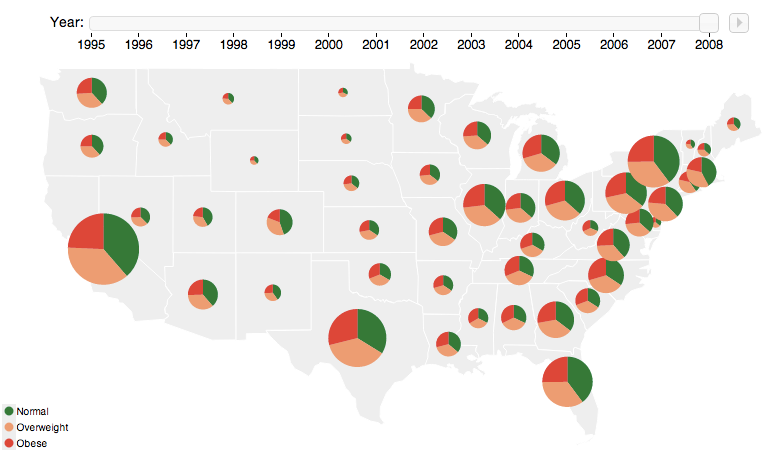
\includegraphics[width=0.5\textwidth]{images/grundlagen-symbol_map.png}
   \caption{Symbol Map}
   \label{figure:symbol_map}
\end{figure}

% dense pixel displays

\textbf{Dense Pixel} Visualisierungen assoziieren jeden Wert einer Dimension mit einem eingefärbten Pixel und platzieren die Pixel einer Dimension nebeneinander. Ein Beispiel dafür ist das Recursive Pattern \cite{Keim1995} (Abbildung~\ref{figure:recursive_pattern}).

\begin{figure}[htbp]
   \centering
   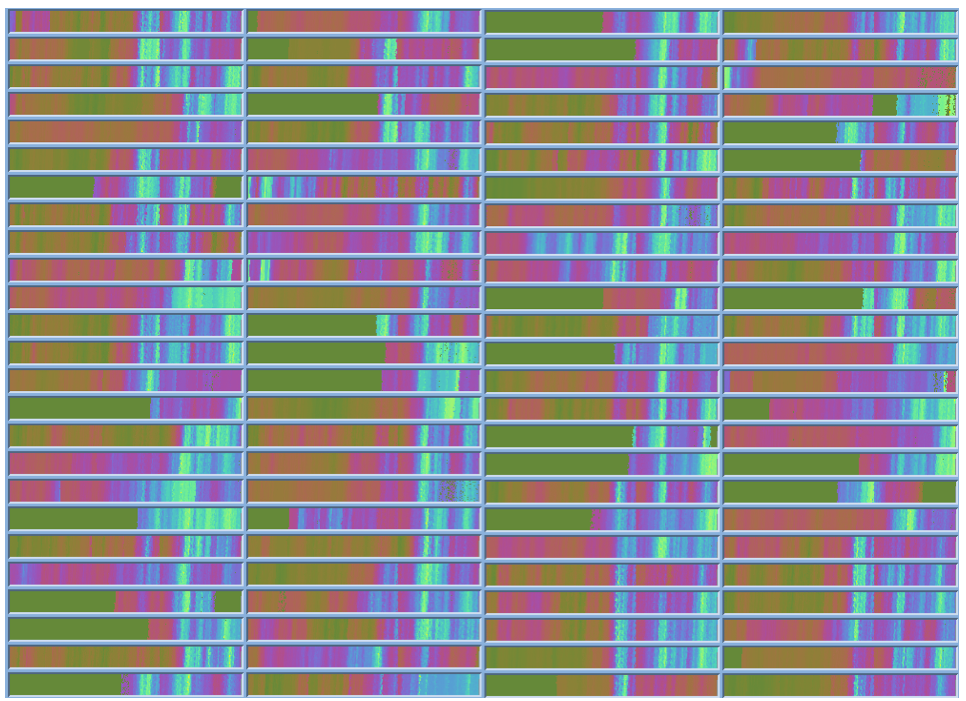
\includegraphics[width=0.5\textwidth]{images/grundlagen-recursive_pattern.png}
   \caption{Recursive Pattern}
   \label{figure:recursive_pattern}
\end{figure}

% stacked displays

\textbf{Verschachtelte} Visualisierungen repräsentieren Hierarchien, wobei Kindknoten innerhalb ihrer Eltern dargestellt werden. Beispiele dafür sind Treemaps \cite{Shneiderman1992} oder Nested Circles (Abbildung~\ref{figure:nested_circles}).

\begin{figure}[htbp]
   \centering
   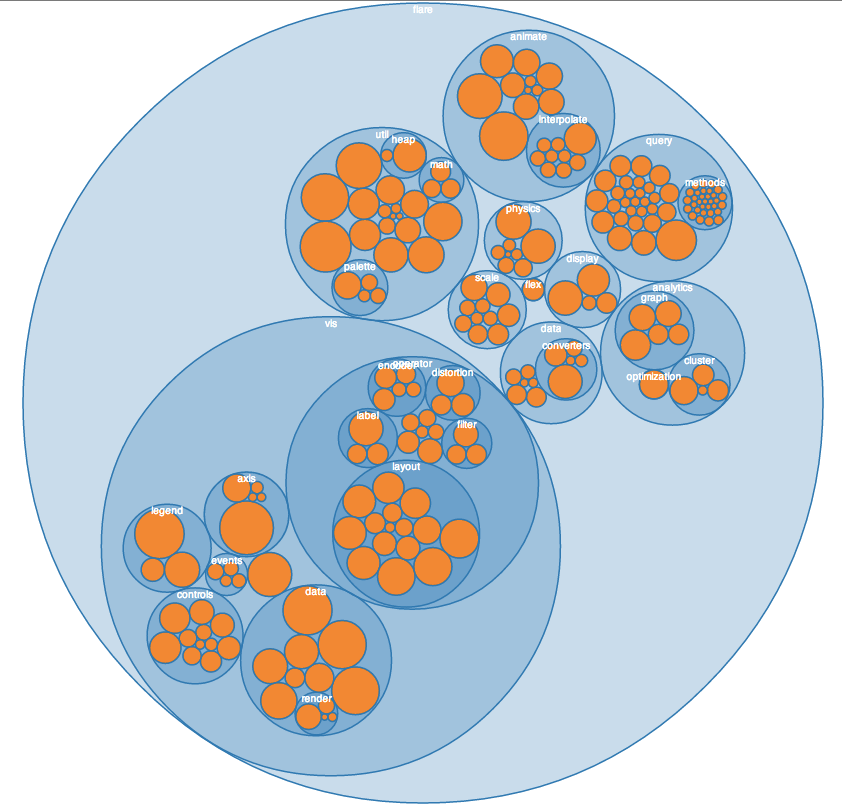
\includegraphics[width=0.25\textwidth]{images/grundlagen-nested_circles.png}
   \caption{Nested Circles}
   \label{figure:nested_circles}
\end{figure}

\subsubsection{Interaktionstechniken}
\label{section:standderforschung:grundlagen:informationsvisualisierung:interaktionstechniken}

% dynamische projektionen

\textbf{Dynamische Projektionen} zeigen dem Benutzer automatisch beispielsweise verschiedene Scatterplots des Datensatzes. Diese Interaktionstechnik eignet sich besonders für multidimensionale Datensätze. Umgesetzt wurde sie zum Beispiel in XGobi \cite{Swayne1998}.

% interaktives filtern

Durch \textbf{interaktives Filtern} bestimmt der Benutzer, welche Teilmenge des Datensatzes visualisiert wird. Das kann durch direktes Auswählen (Browsing) oder durch Bestimmen von Eigenschaften der gewünschten Daten (Querying) passieren. Letzteres ist in modernen E-Commerce-Systemen durch Facetten \cite{Yee2003} umgesetzt (Abbildung~\ref{figure:faceted_browsing}).

\begin{figure}[htbp]
   \centering
   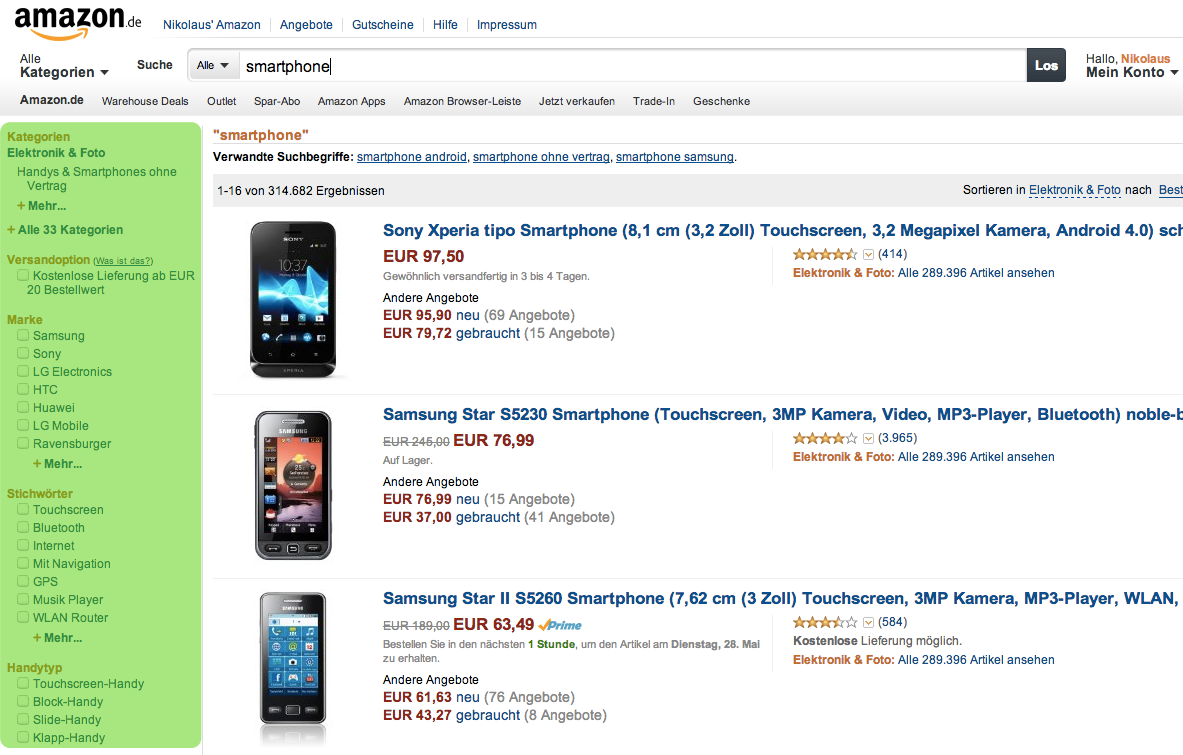
\includegraphics[width=0.5\textwidth]{images/grundlagen-faceted_browsing.png}
   \caption{Faceted Browsing bei Amazon.de}
   \label{figure:faceted_browsing}
\end{figure}

% interaktives zoomen

\textbf{Interaktives Zoomen} ermöglicht es dem Benutzer mehr oder weniger Details anzuzeigen. Damit ist nicht nur der computergrafische Vorgang der Skalierung gemeint (wie etwa bei einem Mikroskop), sondern auch schlecht sichtbare Elemente auszublenden (wie z.\,B. bei Google Maps, siehe Abbildung~\ref{figure:zoom}).

\begin{figure}[htbp]
   \centering
   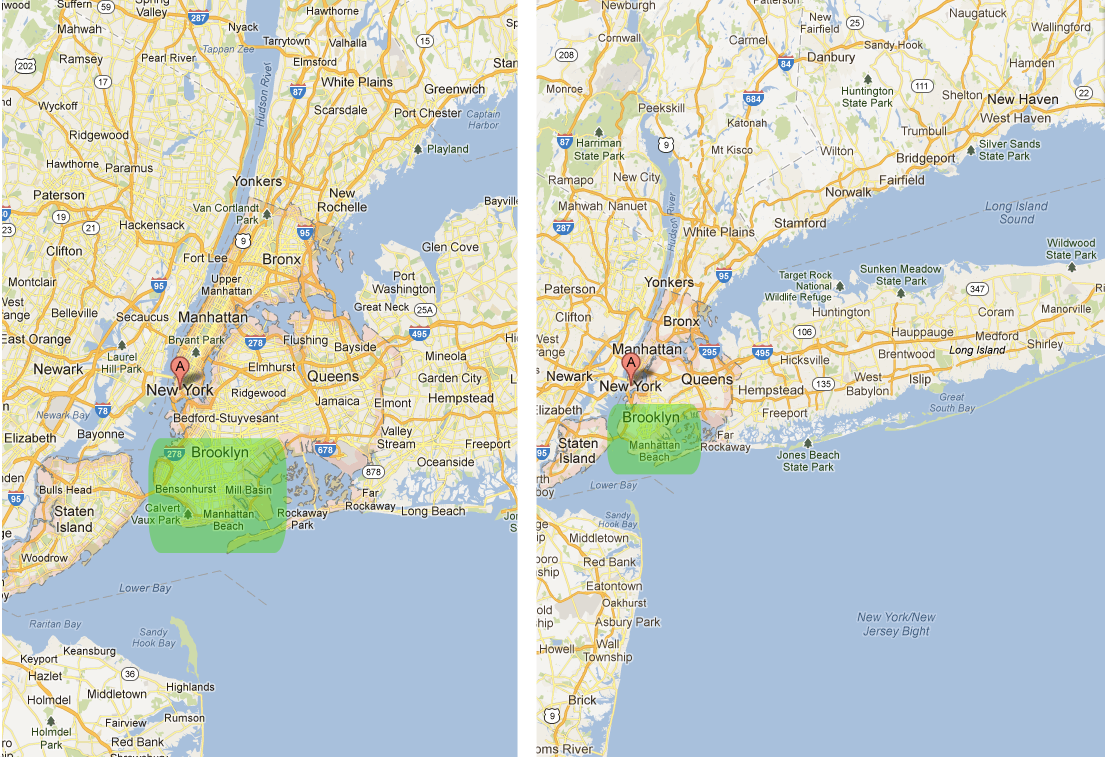
\includegraphics[width=0.5\textwidth]{images/grundlagen-zoom.png}
   \caption{Interaktiver Zoom bei Google Maps: Im rechten, ausgezoomten Bild fehlt beispielsweise die Interstate 278 (grüne Markierung)}
   \label{figure:zoom}
\end{figure}

% distortion (fisheyes and such)

Durch \textbf{Verzerrung} kann ein Bereich der Visualisierung mit hohem Detailgrad angezeigt werden, während der Rest nur wenig detailliert sichtbar ist. Ein bekanntes Beispiel dafür ist das Fisheye (Abbildung~\ref{figure:fisheye}).

\begin{figure}[htbp]
   \centering
   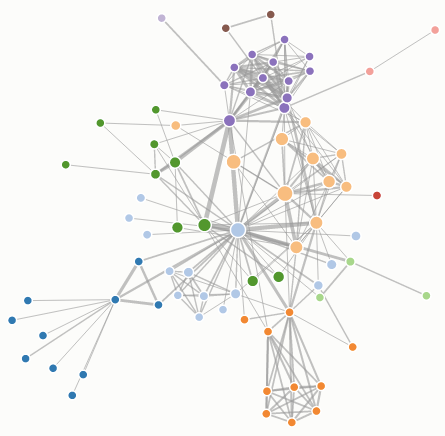
\includegraphics[width=0.5\textwidth]{images/grundlagen-fisheye.png}
   \caption{Fisheye: Das Zentrum der Verzerrung befindet sich ungefähr beim hellblauen Knoten in der Mitte}
   \label{figure:fisheye}
\end{figure}

% link & brush

\textbf{Linking \& Brushing} wird vor allem bei mehreren verschiedenen Visualisierungen eingesetzt. Die in einer Visualisierung markierten Daten werden auch in allen anderen Visualisierungen hervorgehoben. Das können zum Beispiel Scatterplots (siehe multidimensionale Visualisierungen in Abschnitt~\ref{section:standderforschung:informationsvisualisierung:visualisierungstechniken}), verschiedene Histogramme (Abbildung~\ref{figure:link_brush}\footnote{\url{http://square.github.io/crossfilter/}}) oder gemischte Visualisierungen sein.

\begin{figure}[htbp]
   \centering
   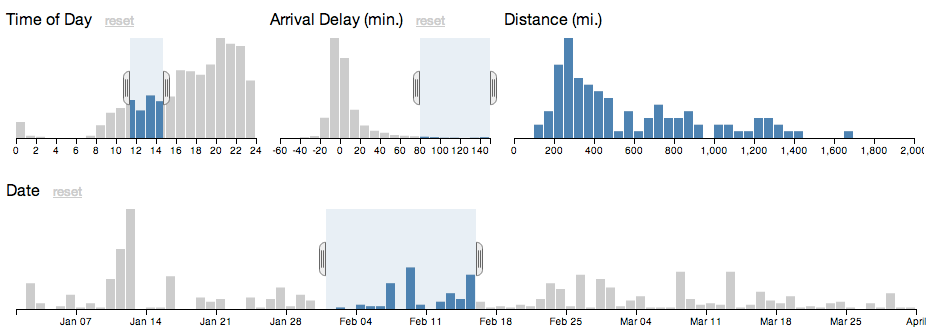
\includegraphics[width=0.75\textwidth]{images/grundlagen-link_brush.png}
   \caption{Linking \& Brushing bei Crossfilter.js: Ausgewählt wurden Flüge mit mehr als 80 Minuten Verspätung, die betroffenen Bereiche in anderen Histogrammen wurden automatisch markiert.}
   \label{figure:link_brush}
\end{figure}

todo: Was habe ich daraus jetzt gelernt?

\subsection{User Assistance}
\label{section:standderforschung:grundlagen:user_assistance}

% was ist assistance?

Der Begriff \enquote{User Assistance} steht für verschiedene Möglichkeiten, einem Benutzer zu helfen seine Ziele zu erreichen. Gapenne et al. \cite{Gapenne2002} definieren vier Beziehungstypen zwischen Mensch und Technologie, welche auch konkret auf Software übertragen werden können. Einer davon ist Assistance:

\begin{quote}
The assistance relationship appears as a sub-category of supplementation since it is not a crucial one for the actual and main activity. The function of this type of technology is to qualify and display the state and/or the becoming of the supplementation device which the subject is engaged in.
\end{quote}

Assistance sind also zum Beispiel eine Einparkhilfe im Auto oder eine Eieruhr in der Küche: Erfolgreiches Einparken oder Kochen ist auch ohne sie möglich, aber leichter mit ihnen. Supplementation hingegen erweitert die Fähigkeiten des Anwenders, also zum Beispiel eine Handprothese mit der die Pfanne angefasst werden kann.

% wie kann man assistance klassifizieren?

Rech et al. \cite{Rech2007} beschreiben intelligente Assistance in der Softwareentwicklung. Prinzipiell müssen zuerst Daten gesammelt werden, bevor die Assistance generiert und angeboten werden kann (Abbildung~\ref{figure:intelligent_assistance}). Folgende Punkte müssen in den einzelnen Schritten beachtet werden.

\begin{itemize}

	\item Daten sammeln
	\begin{itemize}
		\item Welche Datenquellen sollen benutzt werden?
		\item Wann soll die Datenanalyse stattfinden?
		\item Wie können Erkenntnisse aus den Daten gewonnen werden?
	\end{itemize}
	\item Assistance generieren
	\begin{itemize}
		\item Für wen ist die Assistance gedacht?
		\item Was soll durch Assistance erweitert werden?
		\item Für welchen Prozess/Vorgang ist die Assistance gedacht?
		\item Was ist die Zielumgebung der Assistance?
	\end{itemize}
	\item Assistance anbieten
	\begin{itemize}
		\item Wann soll Asssistance angeboten werden?
		\item Welche Modalität (visuell, akustisch usw.) soll die Assistance anbieten?
		\item Wo soll die Information angezeigt werden?
		\item Warum muss dem Benutzer geholfen werden?
	\end{itemize}
\end{itemize}

\begin{figure}[htbp]
   \centering
   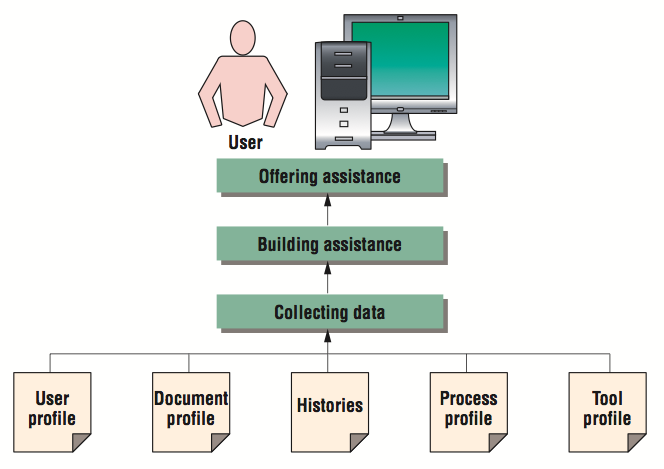
\includegraphics[width=0.5\textwidth]{images/grundlagen-intelligent_assistance.png}
   \caption{Intelligente Assistance nach \cite{Rech2007}}
   \label{figure:intelligent_assistance}
\end{figure}

Besonders die Modalität der Assistance erscheint von großer Bedeutung für eine schnelle und effektive Wissensaufnahme. Wie Information wahrgenommen wird, hat Auswirkungen sowohl auf Verständnis (\enquote{Ein Bild sagt mehr als tausend Worte}) als auch auf die benötigte Zeit. Tausend Worte können auf der Suche nach relevanten Informationen immer noch überflogen werden, eine zehnminütige akustische Hilfestellung nicht.

% effektivität von textuellen, akustischen, visuellen, gemischten erklärungen

Da kein Medium (Film, Audio, Buch etc.) besser zum Lernen geeignet ist als ein anderes \cite{Clark1994, Kozma1994} und multimodale Erklärungen effektiver als monomodale sind \cite{Mayer2002}, stellt sich die Frage, wie Multimedia-Hilfe konstruiert werden soll. Dazu kann auf die kognitive Multimedia-Lerntheorie zurückgegriffen werden. Sie geht davon aus, dass Menschen Wissen grundsätzlich über zwei Kanäle (visuell und verbal) aufnehmen, entsprechende Repräsentationen bilden und mit vorhandenem Wissen verknüpfen (Abbildung~\ref{figure:kognitive_multimedia_lerntheorie}). Die beiden Aufnahmekanäle sind in ihrer Kapazität beschränkt. Müssen zu viele Informationen verarbeitet werden, kommt es zum \enquote{Cognitive Overload} und die Lernfähigkeit wird eingeschränkt. Daraus ergeben sich vier Richtlinien zur Kontruktion der Multimedia-Erklärungen:

\begin{itemize}
	\item \textbf{Gleichzeitigkeit}: Werden akustische und visuelle Mittel eingesetzt, so sollen sie gleichzeitig präsentiert werden \cite{Mayer1991}. So können Lernende ihre visuellen und verbalen Wissensrepräsentationen besser miteinander verknüpfen.
	\item \textbf{Prägnanz}: Unterhaltsame aber irrelevante Details fördern die Erinnerungsfähigkeit an einen Text nicht \cite{Garner1989}. Deswegen sollen nur relevante Informationen vermittelt werden.
	\item \textbf{Multimodalität}: Informationen sollten möglichst auf visuelle und verbale Art vermittelt werden, um zu verhindern, dass ein Aufnahmekanal überlastet wird (bspw. durch die Darstellung einer Animation mit On-Screen-Text) \cite{Moreno1999}.
	\item \textbf{Keine Redundanz}: Aus dem selben Grund warum zweikanälige Erklärungen vorzuziehen sind, sollte auch Redundanz in einem Aufnahmekanel vermieden werden.
\end{itemize}

\begin{figure}[htbp]
   \centering
   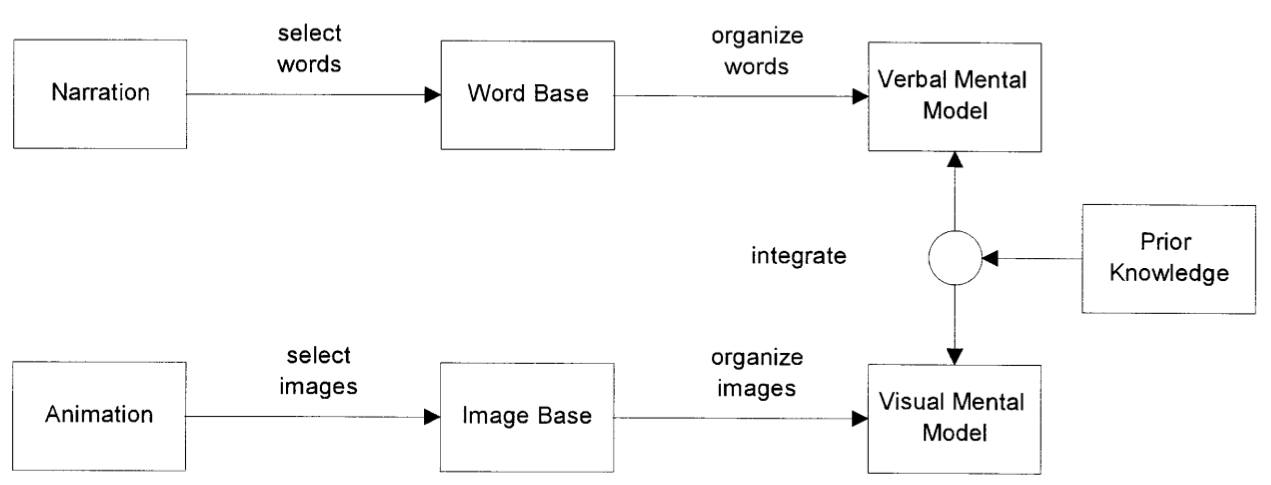
\includegraphics[width=0.75\textwidth]{images/grundlagen-kognitive_multimedia_lerntheorie.png}
   \caption{Kognitive Multimedia-Lerntheorie nach \cite{Mayer2002}}
   \label{figure:kognitive_multimedia_lerntheorie}
\end{figure}

% user assistance möglichkeiten für jede modalität

Wie kann User Assistance im visuellen bzw. verbalen Aufnahmekanal aussehen? Verbale Erklärungen können zur Laufzeit generiert werden \cite{Bauer2011, Gesell2012, Matheson2012}, sind jedoch tendenziell zu langatmig formuliert und enthalten viele Wiederholungen. Auf Grund der vorhin erwähnten Designprinzipien \enquote{Prägnanz} und \enquote{Keine Redundanz} sollte davon wahrscheinlich abgesehen und verbale Erklärungen handgeschrieben oder sehr kurz gehalten werden.

Die naheliegendste Möglichkeit für visuelle User Assistance sind Bilder. Illustrationen/Schemata sind in der Tat hilfreich, solange sowohl die Bestandteile des Systems (z.\,B. eine Luftpumpe) als auch die einzelnen Schritte des Prozesses (z.\,B. Luft einziehen, Luft auspumpen) dargestellt werden \cite{Mayer1990}. Auch Comics sind gut geeignet um Sachverhalte zu erklären (Beispiele dafür sind u.\,a. \cite{McCloud1994, McCloud2008}) und eine ansprechende Variante für User Assistance \cite{Webb2012}.

Animationen im Sinne von kurzen Videos mit abstrahiertem Inhalt können ebenfalls ein geeigneter Weg sein um Wissen zu vermitteln, sofern die erwähnten Designprinzipien eingehalten werden \cite{Mayer2002a}. Allerdings ist es möglich, dass Benutzer mit wenig Vorwissen weniger davon profitieren also solche mit viel Vorwissen \cite{Kalyuga2008}. Wenn Animationen eingesetzt werden, sollte den Benutzern Kontrolle über die Geschwindigkeit der Animation gegeben und wichtige Teile gekennzeichnet werden \cite{Wong2011}. Bei Web User Interfaces besteht die Möglichkeit konkrete Elemente der InfoVis für die Animation heranzuziehen. Das würde dem Prinzip der \enquote{Semantic Transparency} \cite{Kohlhase2009} entsprechen, wonach Benutzer möglichst direkt auf den für ihre Ziele relevanten UI-Elementen arbeiten sollen.

Filme? Hier gibt es eine Doktorarbeit, aber die finde ich online nicht \url{http://search.proquest.com/docview/1286857518}. Ansonsten scheint sich damit niemand so richtig zu beschäftigen und eigentlich ist es mir auch wurscht weil Tutorialvideos einen immer so aus dem Arbeitskontext reissen. Ich könnte es mit einer Quelle ausschließen, wenn ich die wieder finden würde... Da steht sinngemäß drin, dass Hilfe gut ist, wenn man fix wieder in den Arbeitskontext zurückkommt.


\subsubsection{Sensemaking}
\label{section:standderforschung:grundlagen:user_assistance:sensemaking}

% was ist der unterschied zwischen learning und sensemaking?
Im vorhergehenden Abschnitt wurde der Prozess der Wissensvermittlung betrachtet. Um Wissen dauerhaft aufzunehmen, müssen Lernende den Inhalt \emph{verstehen}. Der Begriff \enquote{Understanding} (gleichbedeutend mit Sensemaking) wird angewandt, wenn das Gehirn mehr Elemente des Inhalts (z.\,B. Variablen einer Gleichung) verarbeiten muss als ins Arbeitsgedächtnis passen \cite{Sweller1998}. \emph{Verstanden} hat der Lernende dann, wenn diese Elemente zu einem sogenannten Schema (mentales Modell) verarbeitet wurden und als ein einziges Element im Arbeitsgedächtnis gehalten werden können (z\,B. eine komplexe Zahl statt drei Variablen $a$, $b$ und $i$).

% wie funktioniert der prozess der wissensaneignung?

Klein \cite{Klein2006a} beschreibt in seinem Data/Frame-Modell (Abbildung~\ref{figure:data_frame_model}), wie dieser Prozess funktioniert. \enquote{Data} beschreibt dabei die Elemente des Inhalts und \enquote{Frame} das mentale Modell oder Schema. Ähnlich dem Visual Analytics Process (Abschnitt~\ref{section:standderforschung:informationsvisualisierung}) ist Sensemaking ein iterativer Prozess, aber ohne wirklichen Anfang oder Ende. Der Lernende startet mit einem Frame, versucht die Daten einzupassen und nimmt Anpassungen vor bzw. verwirft ein Frame, wenn es nicht weiter durch Daten gestützt wird. Dabei sollte der Lernende möglichst selbstständig einer Lösung kommen, nicht zu viele Daten gleichzeitig sehen und während des Prozesses keine Hypothesen aufstellen müssen, die nicht überprüft werden können \cite{Klein2006}.

\begin{figure}[htbp]
   \centering
   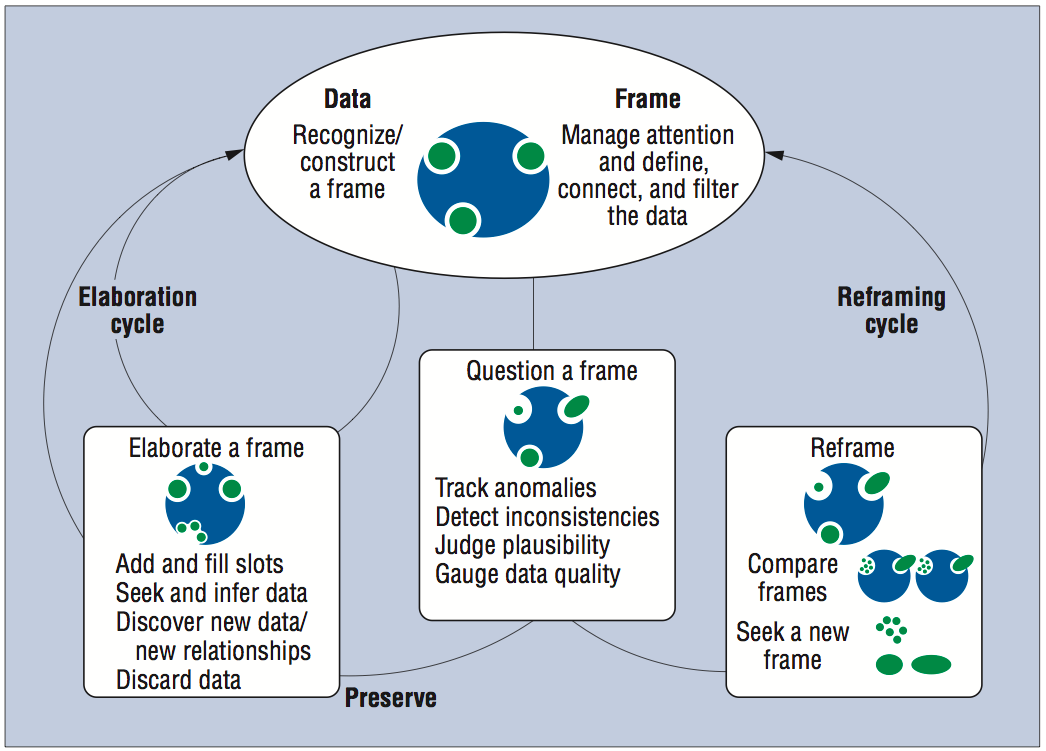
\includegraphics[width=0.75\textwidth]{images/grundlagen-data_frame_model.png}
   \caption{Data/Frame Modell nach \cite{Klein2006}}
   \label{figure:data_frame_model}
\end{figure}

% was ist dabei zu beachten?

Während des Verständnisprozesses ist es außerdem hilfreich, Wissen in irgendeiner Form externalisieren zu können, beispielsweise mit Hilfe einer Mind Map \cite{Qu2005, Novak2007, Umapathy2010}. Andere Menschen können dadurch auf bereits durchgeführte Verständnisprozesse anderer aufbauen, wobei die Struktur aber wichtiger ist als der tatsächliche Inhalt \cite{Fisher2012}.

Nachdem betrachtet wurde, wie Verständnis funktioniert, stellt sich die Frage, \emph{was} vermittelt werden soll um Menschen mit wenig InfoVis-Erfahrung zu helfen. Dazu gehört laut Grammel \cite[S. 127]{Grammel2012} unter anderem das mentale Modell des Benutzers zu verwenden, beispielsweise indem dieselben Bezeichnungen verwendet werden, und zu lehren, wie Visualisierungen verwendet und interpretiert werden.

\section{Verwandte Arbeiten}
\label{section:standderforschung:verwandte_arbeiten}

In diesem Abschnitt werden verwandte Arbeiten behandelt.

\subsection{Webbasierte Mashup Plattformen}

Es existieren ein paar andere Mashup-Plattformen als VizBoard, aber ich bin mir nicht sicher, ob die tatsächlich in meine Arbeit gehören. Ich entwickle kein Mashup.

Yahoo Pipes\footnote{\url{http://pipes.yahoo.com/pipes/}}

Apache Rave\footnote{\url{http://rave.apache.org/}}

DashMash \cite{Cappiello2011}


\subsection{Visualisierungstools}

infogr.am\footnote{\url{http://infogr.am/}} ermöglicht es Benutzern, statische Infografiken und Charts zu erstellen. Die dargestellten Daten sind in einer Tabelle enthalten, die hochgeladen und online bearbeitet werden kann. Danach kann die Visualisierung veröffentlicht und in Social Networks gepostet werden. Der Webservice besitzt nur eingeschränkte Funktionalität, ist aber einfach zu benutzen und sieht gut aus, was für Endnutzer eine gute Kombination ist.

Weave\footnote{\url{http://oicweave.org/}} ist eine Webapplikation, mit der Benutzer ein Mashup aus Visualisierungen erstellen können. Mögliche Datenquellen sind strukturierte Daten wie Tabellen und CSV Dateien. Benutzer können aus verschiedenen Visualisierungen wählen und diese an Daten binden. Das User Interface (Abbildung~\ref{figure:weave}) ist allerdings sehr komplex und Hilfe gibt es nur in Form einer Online-Dokumentation und einem kurzen Tutorialvideo.

\begin{figure}[htbp]
   \centering
   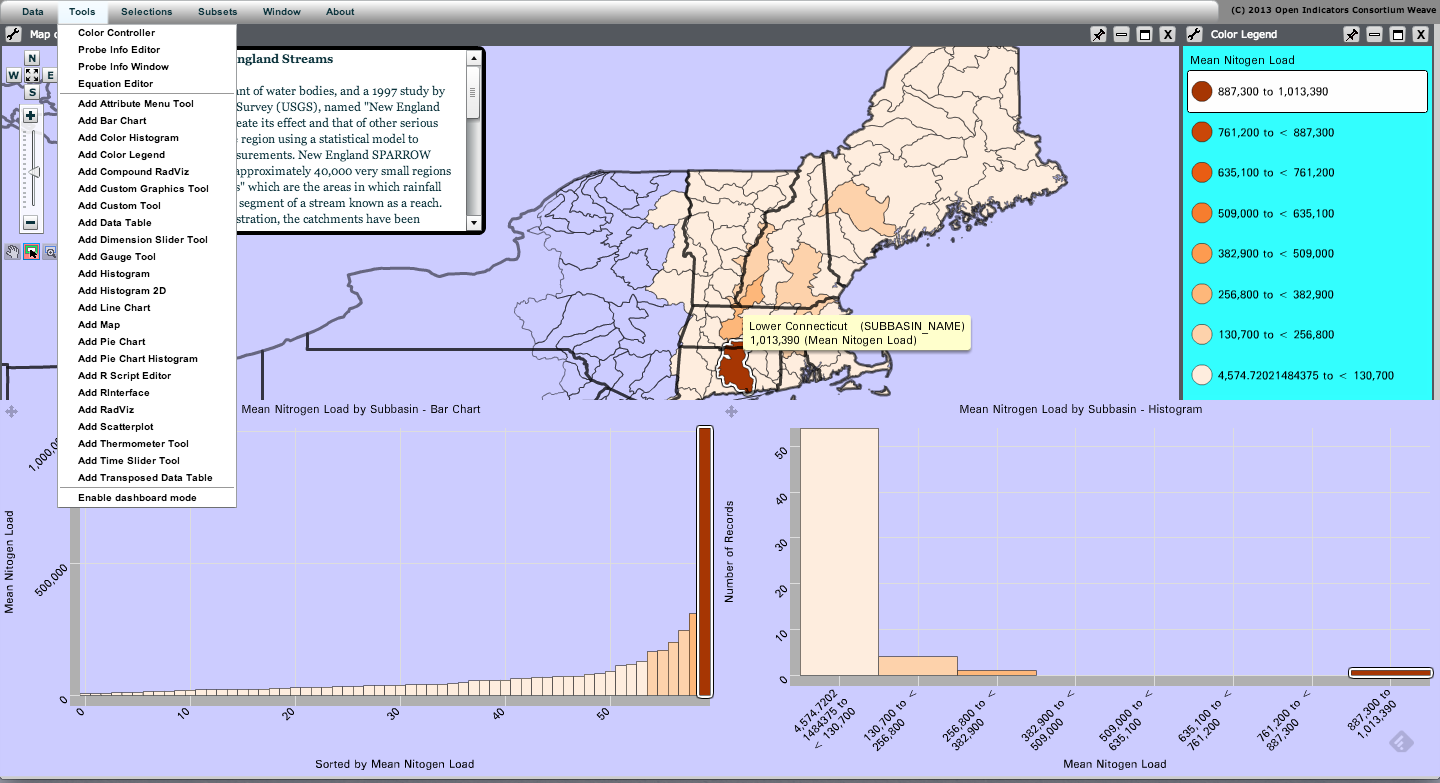
\includegraphics[width=0.75\textwidth]{images/verwandte_arbeiten-weave.png}
   \caption{Weave User Interface}
   \label{figure:weave}
\end{figure}

Tableau\footnote{\url{http://www.tableausoftware.com/}} ist eine Desktopapplikation, mit der aus Tabellen oder Datenbanken Diagramme erstellt werden können. Dabei wird das Prinzip von \enquote{Semantic Transparency} umgesetzt, weil der Benutzer die zu visualisierenden Daten per Drag \& Drop auf dem Diagramm platziert. \textbf{Und?}

\subsubsection{Sensemaking}

% Sandbox \cite{Wright2006} ist ein Prototyp einer Desktopanwendung, die den Prozess des Sensemakings unterstützen soll. Dazu kann der Benutzer Informationen ähnlich Post-Its auf einer Canvas anordnen und mit Hilfe von Gesten gruppieren, Platz schaffen oder löschen. Informationsvisualisierungen kommen dabei nicht zum Einsatz.

Groth und Streefkerk \cite{Groth2006} präsentieren ein generisches Annotationssystem für Informationsvisualisierungen am Beispiel einer 3D Visualisierung von Molekülen. Grundlage des Systems sind Nutzerinteraktionen wie \enquote{rotieren}, \enquote{zoomen} etc., welche geloggt und als Graph abgespeichert werden. An den Knoten des Graphen -- Zustände der InfoVis -- können beliebig viele Kommentare abgelegt werden. Es ist allerdings nicht möglich, innerhalb dieser Sichten noch einmal Elemente zu referenzieren (z.\,B. ein bestimmtes Atom), weswegen das System am besten für InfoVis mit uneingeschränkter Navigation geeignet ist.

Heer et al. \cite{Heer2007} entwickelten mit sense.us einen Prototyp zur asynchronen Kollaboration mit interaktiven Visualisierungen. Benutzer können Kommentare zu Visualisierungen hinzufügen und sie mit grafischen Annotationen (z.\,B. geometrische Formen, Pfeile, Text) versehen. Die Kommentare wurden dabei nicht an die Daten selbst, sondern an die Visualisierung, hinzugefügt. Es war aber möglich Kommentare in anderen Visualisierungen zu referenzieren. Die am meisten verwendeten Annotationstypen waren Pfeile und Text.

Ebenfalls erwähnenswert ist ManyEyes \cite{Viegas2007}. Benutzer können Datensätze hochladen und eine aus mehreren vorgegebenen Visualisierungen wählen. Danach können sie ähnlich wie bei sense.us die Visualisierungen kommentieren, es ist allerdings nicht möglich, die Visualisierung selbst zu annotieren. Wie bei sense.us ist immer nur eine InfoVis sichtbar.

Elias und Bezerianos \cite{Elias2012} entwickelten ein Annotations- bzw. Kommentarsystem für Business Intelligence Dashboards. Dafür interviewten sie Domänenexperten und erarbeiteten sieben funktionale Anforderungen an ein annotationsgesütztes Dashboard. Herausforderungen für ihr Konzept, die auch in dieser Arbeit berücksichtigt werden sollten, waren wie mit sich änderndem Kontext (bei dynamischen Daten) umgegangen und Unabhängigkeit von Granularitäten (Jahr/Monat/Tag) gewährleistet werden soll.

\subsection{User Assistance}

Lim und Dey \cite{Lim2010} kategorisieren mögliche Fragestellungen von Nutzern in kontextadaptiven Anwendungen. Dabei ändert die Anwendung abhängig vom Nutzer- bzw. Nutzungskontext ihren Zustand (z.\,B. schaltet Smartphone auf lautlos) und der Benutzer will wissen, warum (z.\,B. weil er Abends in der Oper ist). Grundlage für Lims Ausführungen ist die Annahme, dass der Nutzer nur eingeschränkt Einfluss auf die Arbeitsweise des Systems hat, etwa durch Hinzufügen eigener Regeln. Das ist im letzten Schritt des VizBoard Workflows nicht gegeben, da der Benutzer die Visualisierungskomponenten selbst ausgewählt hat. Die Fragestellungen könnten aber hilfreich sein, wenn es um die Komponenten selbst geht: \enquote{Warum werden gerade diese Daten angezeigt?}

Cao et al. \cite{Cao2010} untersuchten mit Hilfe der Thinking Aloud Methode \cite{vanSomeren1994} das Verhalten von Endnutzern, wenn sie Mashups erstellen, sowie deren Debugging-Strategien, wenn etwas nicht funktioniert. Dazu benutzten sie das inzwischen eingestellte Microsoft Popfly. In ihrer Studie hatten alle Probanden Probleme mit dem Konzept des Datenflusses, also welche Daten wann zwischen welchen Komponenten ausgetauscht werden.

Kuttal et al. \cite{Kuttal2013} entwickelten ein System zur automatischen Fehlererkennung in Yahoo Pipes und ließen Endnutzer damit debuggen. In den danach erarbeiteten Designrichtlinien schlagen sie unter anderem vor keine technische Begriffe zu verwenden und Undo-Möglichkeiten sowie kontextuelle Hilfe anzubieten.

Chowdhury et al. \cite{Chowdhury2012a} stellen eine Erweiterung von Yahoo Pipes vor, die Kompositionspattern vorschlägt und bei Bedarf in das Mashup einbaut.  Dieses \enquote{Programming by example} könnte in VizBoard benutzt werden, um die Komposition noch einmal zu überarbeiten.

Einige Arbeiten, wie z.\,B. \cite{Gesell2012, Matheson2012}, befassen sich mit der Generierung von textuellen Erklärungen. In beiden Arbeiten ist eine formale Repräsentation des Erklärungsgegenstands notwendig, beispielsweise als Baum von Vorbedingungen und \enquote{Ist Teil von} Relationen oder einer Ontologie. In der Evaluation von Matheson et al. merkten einige Probanden an, dass ihre Erklärungen zu langatmig seien.

% bei champin2012 klingt der titel super, aber das szenario ist irgendwie ein komplett anderes

% Kurlander et al. \cite{Kurlander1996} entwickelten einen Algorithmus, mit dem aus einer Chatkonversation automatisch ein Comic erstellt wurde. So what?

Webb et al. \cite{Webb2012} überprüften in einer Nutzerstudie, wie User Assistance in Form eines Comics gegenüber in Form einer PowerPoint-Präsentation angenommen wird. Comics lagen in allen Fragestellungen (Einfach zu verwenden, attraktiv, nützlich, verständlich) vorne, am Besten wurden Comics angenommen, die eine Metapher beinhalteten.

Forsell und Johansson \cite{Forsell2010} führten eine Nutzerstudie durch, um aus verschiedenen Heuristiken zur Heuristischen Evaluation \cite{Nielsen1994} diejenigen herauszufiltern, welche bei Informationsvisualisierungen hilfreich sind. Darunter finden sich Support für Undo/Redo, visuelle Konsistenz und den mentalen Aufwand des Nutzers gering zu halten.

Grammel \cite{Grammel2012} verfasste seine Doktorarbeit zum Thema, wie InfoVis-Anfänger Visualisierungen konstruieren. Um sie dabei zu unterstützen, schlägt er unter anderem vor, ihr mentales Modell zu verwenden (z.\,B. mit ihnen bekannten Begriffen) und es ihnen zu erleichtern, mehr über InfoVis zu lernen.

Shrinivasan et al. \cite{Shrinivasan2008} entwickelten ein Framework zur Informationsvisualisierung, welches den menschlichen Verständnisprozess unterstützen soll. Es besteht aus drei verschiedenen Views: Der InfoVis selbst, einem \enquote{Knowledge View} und einem \enquote{Navigation View}. Im Knowledge View kann der Benutzer seine Hypothesen und Analysen verwalten bzw. überprüfen, der Navigation View erlaubt es ihm, zu einem beliebigen Punkt im Laufe der Interaktionen zurück zu gehen. In einer Nutzerstudie fanden die vier Probanden den Knowledge View sehr nützlich.

\section{Zusammenfassung}
\label{section:standderforschung:zusammenfassung}

yay

% ###################################################
\chapter{Konzeption}
\label{chapter:konzeption}

Basierend auf dem Szenario (Abschnitt~\ref{section:standderforschung:szenario}) und den Grundlagen (Abschnitt~\ref{section:standderforschung:grundlagen}) wird ein Konzept zur User Assistance für das webbasierte, komposite Informationsvisualisierungssystem VizBoard erstellt. Die Ziele richten sich dabei nach der Anforderungsanalyse (Abschnitt~\ref{section:standderforschung:anforderungsanalyse}).

\section{Einführung}
\label{section:konzeption:einfuehrung}

Blublublu

\subsection{Rollenmodell}
\label{section:konzeption:einfuehrung:rollenmodell}

Bei der Konzeption spielt eine große Rolle, wer für welche Tätigkeit verantwortlich ist. Um diese Fragen klären zu können, wird an dieser Stelle ein Rollenmodell für VizBoard eingeführt (Abbildung~\ref{figure:rollenmodell}).

\begin{figure}[htbp]
   \centering
   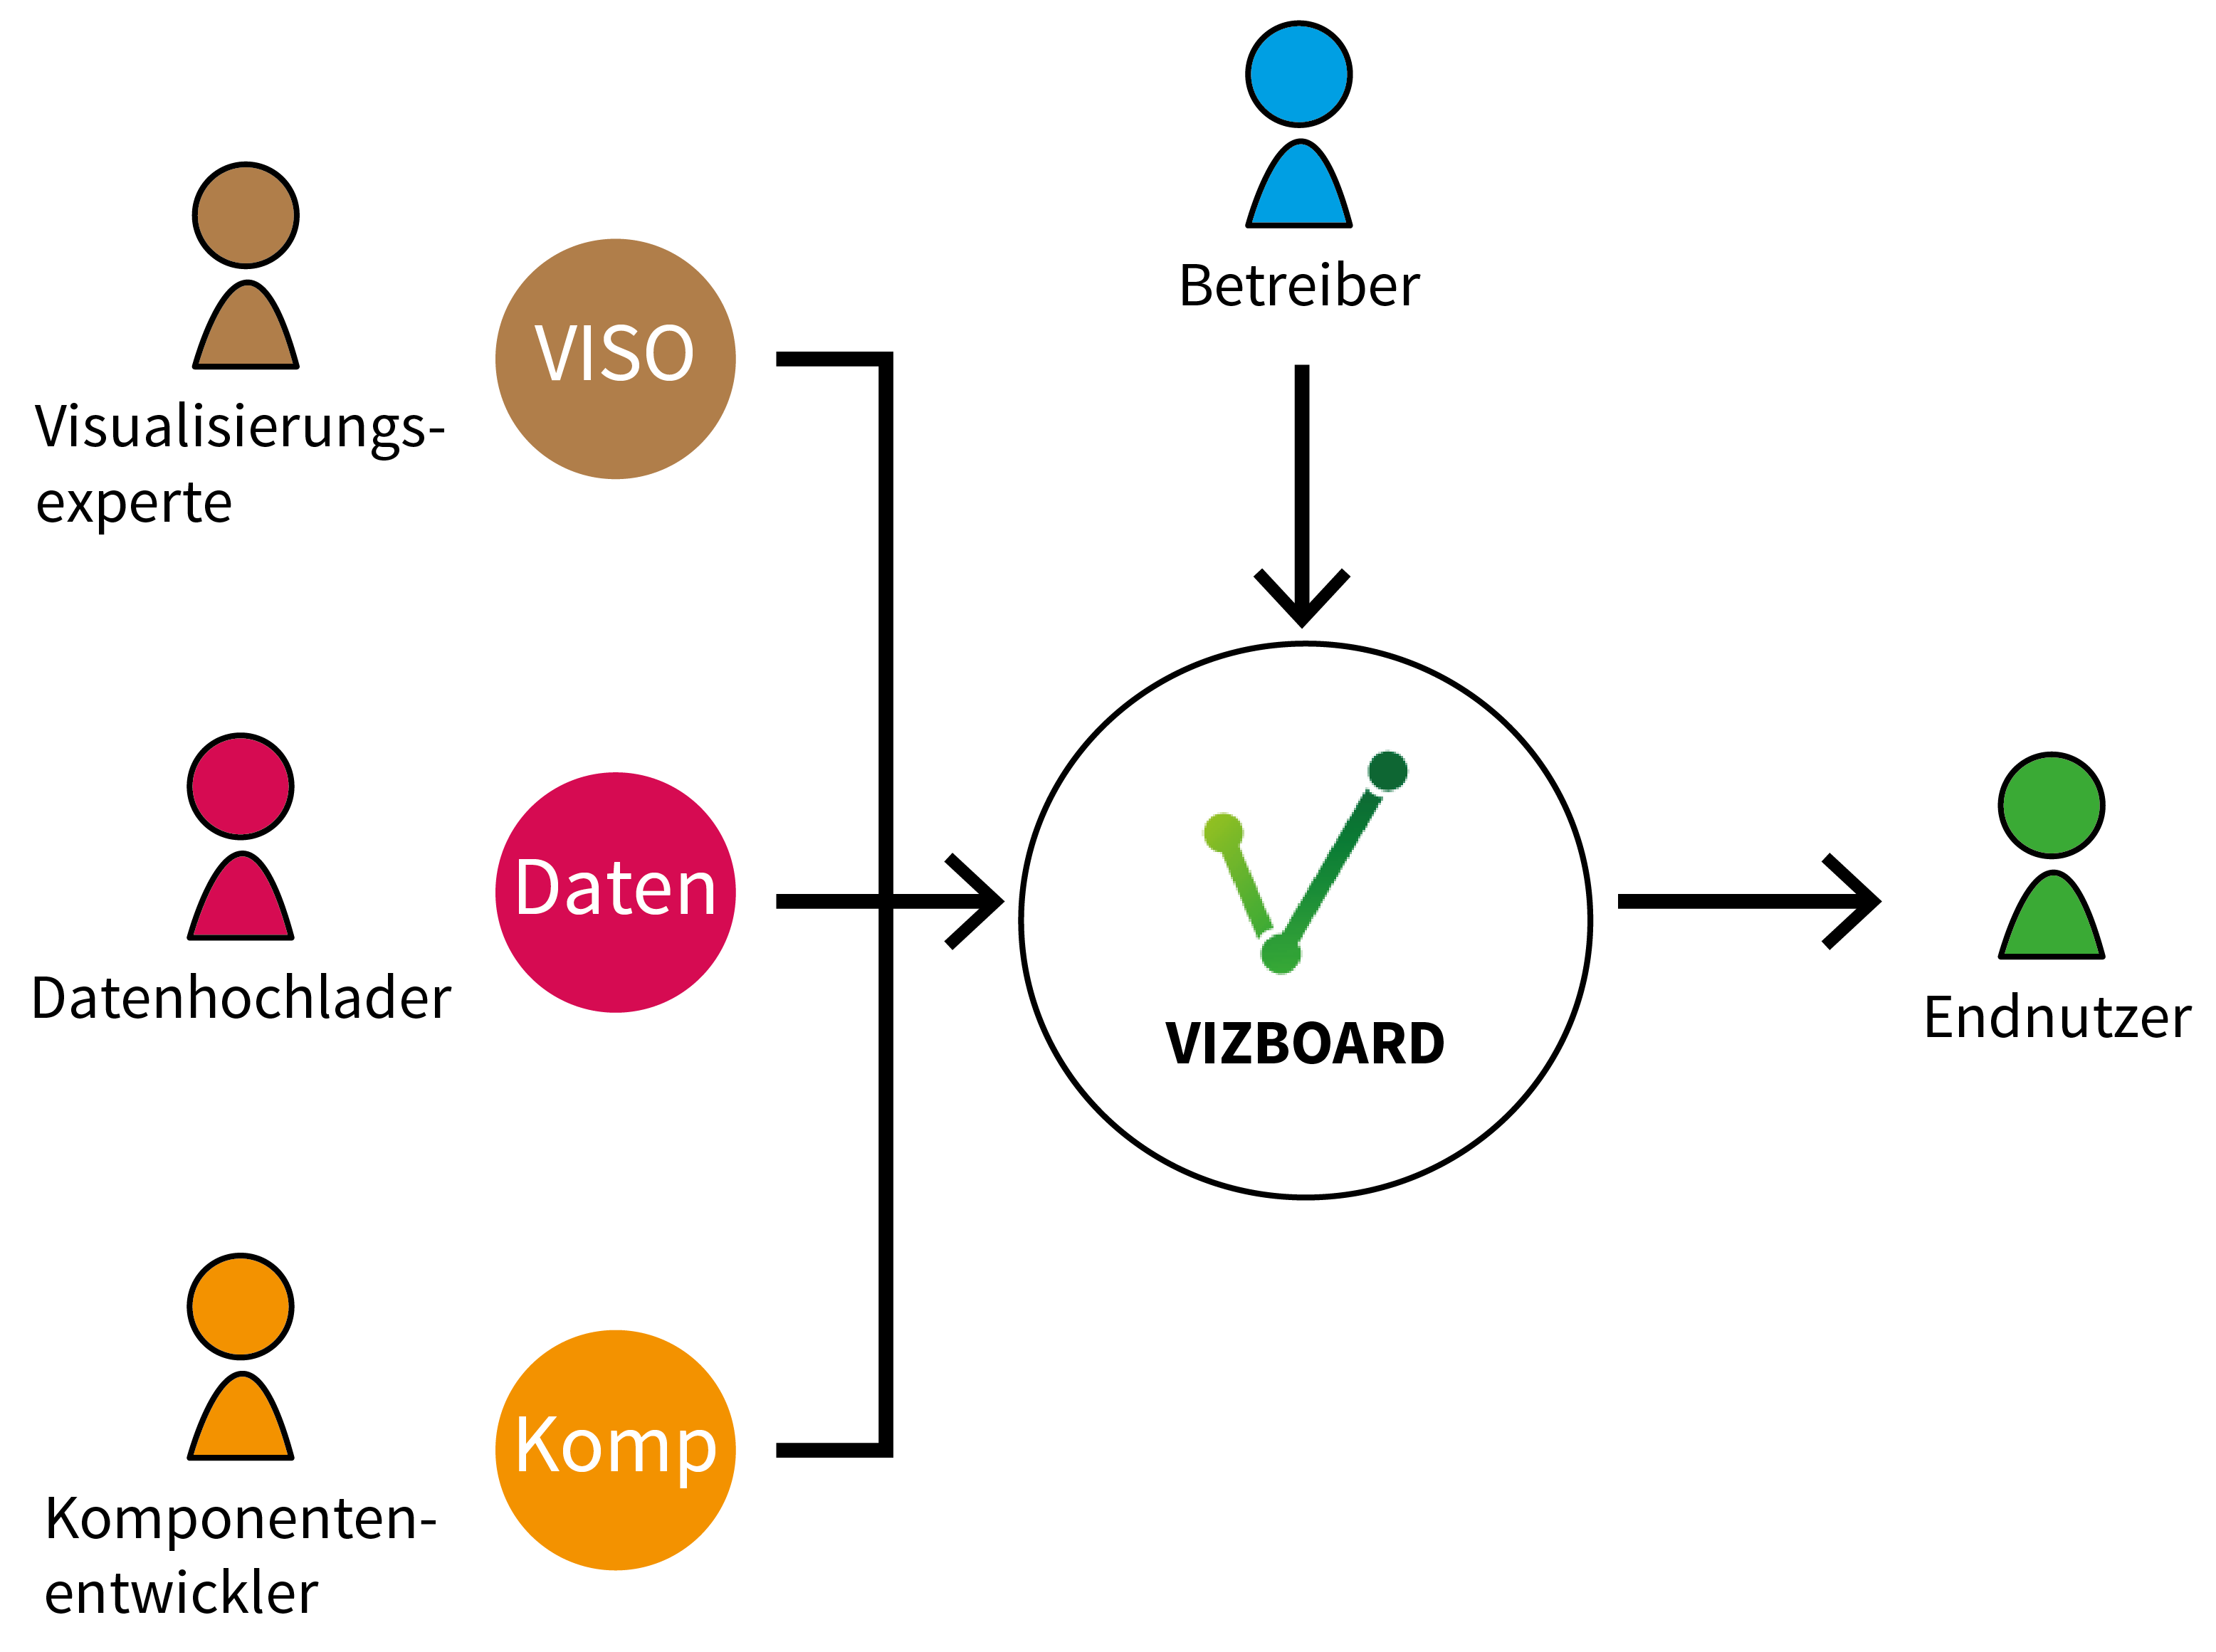
\includegraphics[width=0.5\textwidth]{images/konzeption-rollenmodell.png}
   \caption{Rollenmodell von VizBoard}
   \label{figure:rollenmodell}
\end{figure}

Das System VizBoard muss von jemandem betrieben werden. Der \textbf{Betreiber} bezahlt die Serverkosten und ist für Wartung und Instandhaltung von VizBoard verantwortlich. Für ihn ist wichtig, dass die anderen Parteien zufrieden sind, sodass sein System auch genutzt wird.

VizBoard greift auf die VISO zurück, eine Ontologie von Wissen über Informationsvisualisierung. Der \textbf{Visualisierungsexperte} besitzt Expertenwissen in der Domäne der InfoVis und formalisiert sein es in der VISO, um VizBoard zu verbessern.

Ein wichtiger Teil von VISO sind die vorhandenen Daten. Der \textbf{Datenhochlader} stellt Datensätze in unterschiedlichen Formaten (z\,B. APIs, RDF oder Excel Daten) zur Verfügung, die von Administratoren -- also letztlich dem Betreiber -- in VizBoard hochgeladen werden können.

Ebenso wichtig wie die Daten sind die Komponenten, die sie visualisieren. Sie werden von \textbf{Komponentenentwicklern} geschrieben und bei VizBoard registriert. Komponentenentwickler können programmieren und kennen sich teilweise auch mit InfoVis aus.

Der \textbf{Endnutzer} verwendet VizBoard, um Wissen in semantischen Datensätzen aufnehmen zu können. Er weiß weder über InfoVis noch über semantische Daten Bescheid und verfügt auch nicht über Programmierkenntnisse.

\subsection{User Interface}
\label{section:konzeption:einfuehrung:ui}

Im Laufe der Konzeption werden zum besseren Verständnis einige User Interface Mockups entworfen. Diese basieren auf der Grundlage aus dem Szenario (Abschnitt~\ref{section:standderforschung:szenario}). Die dort erwähnte Komposition enthält eine Karte, eine Treemap, eine Tabelle und ein Balkendiagramm (Abbildung~\ref{figure:ui-grundlage}).

\begin{figure}[htbp]
   \centering
   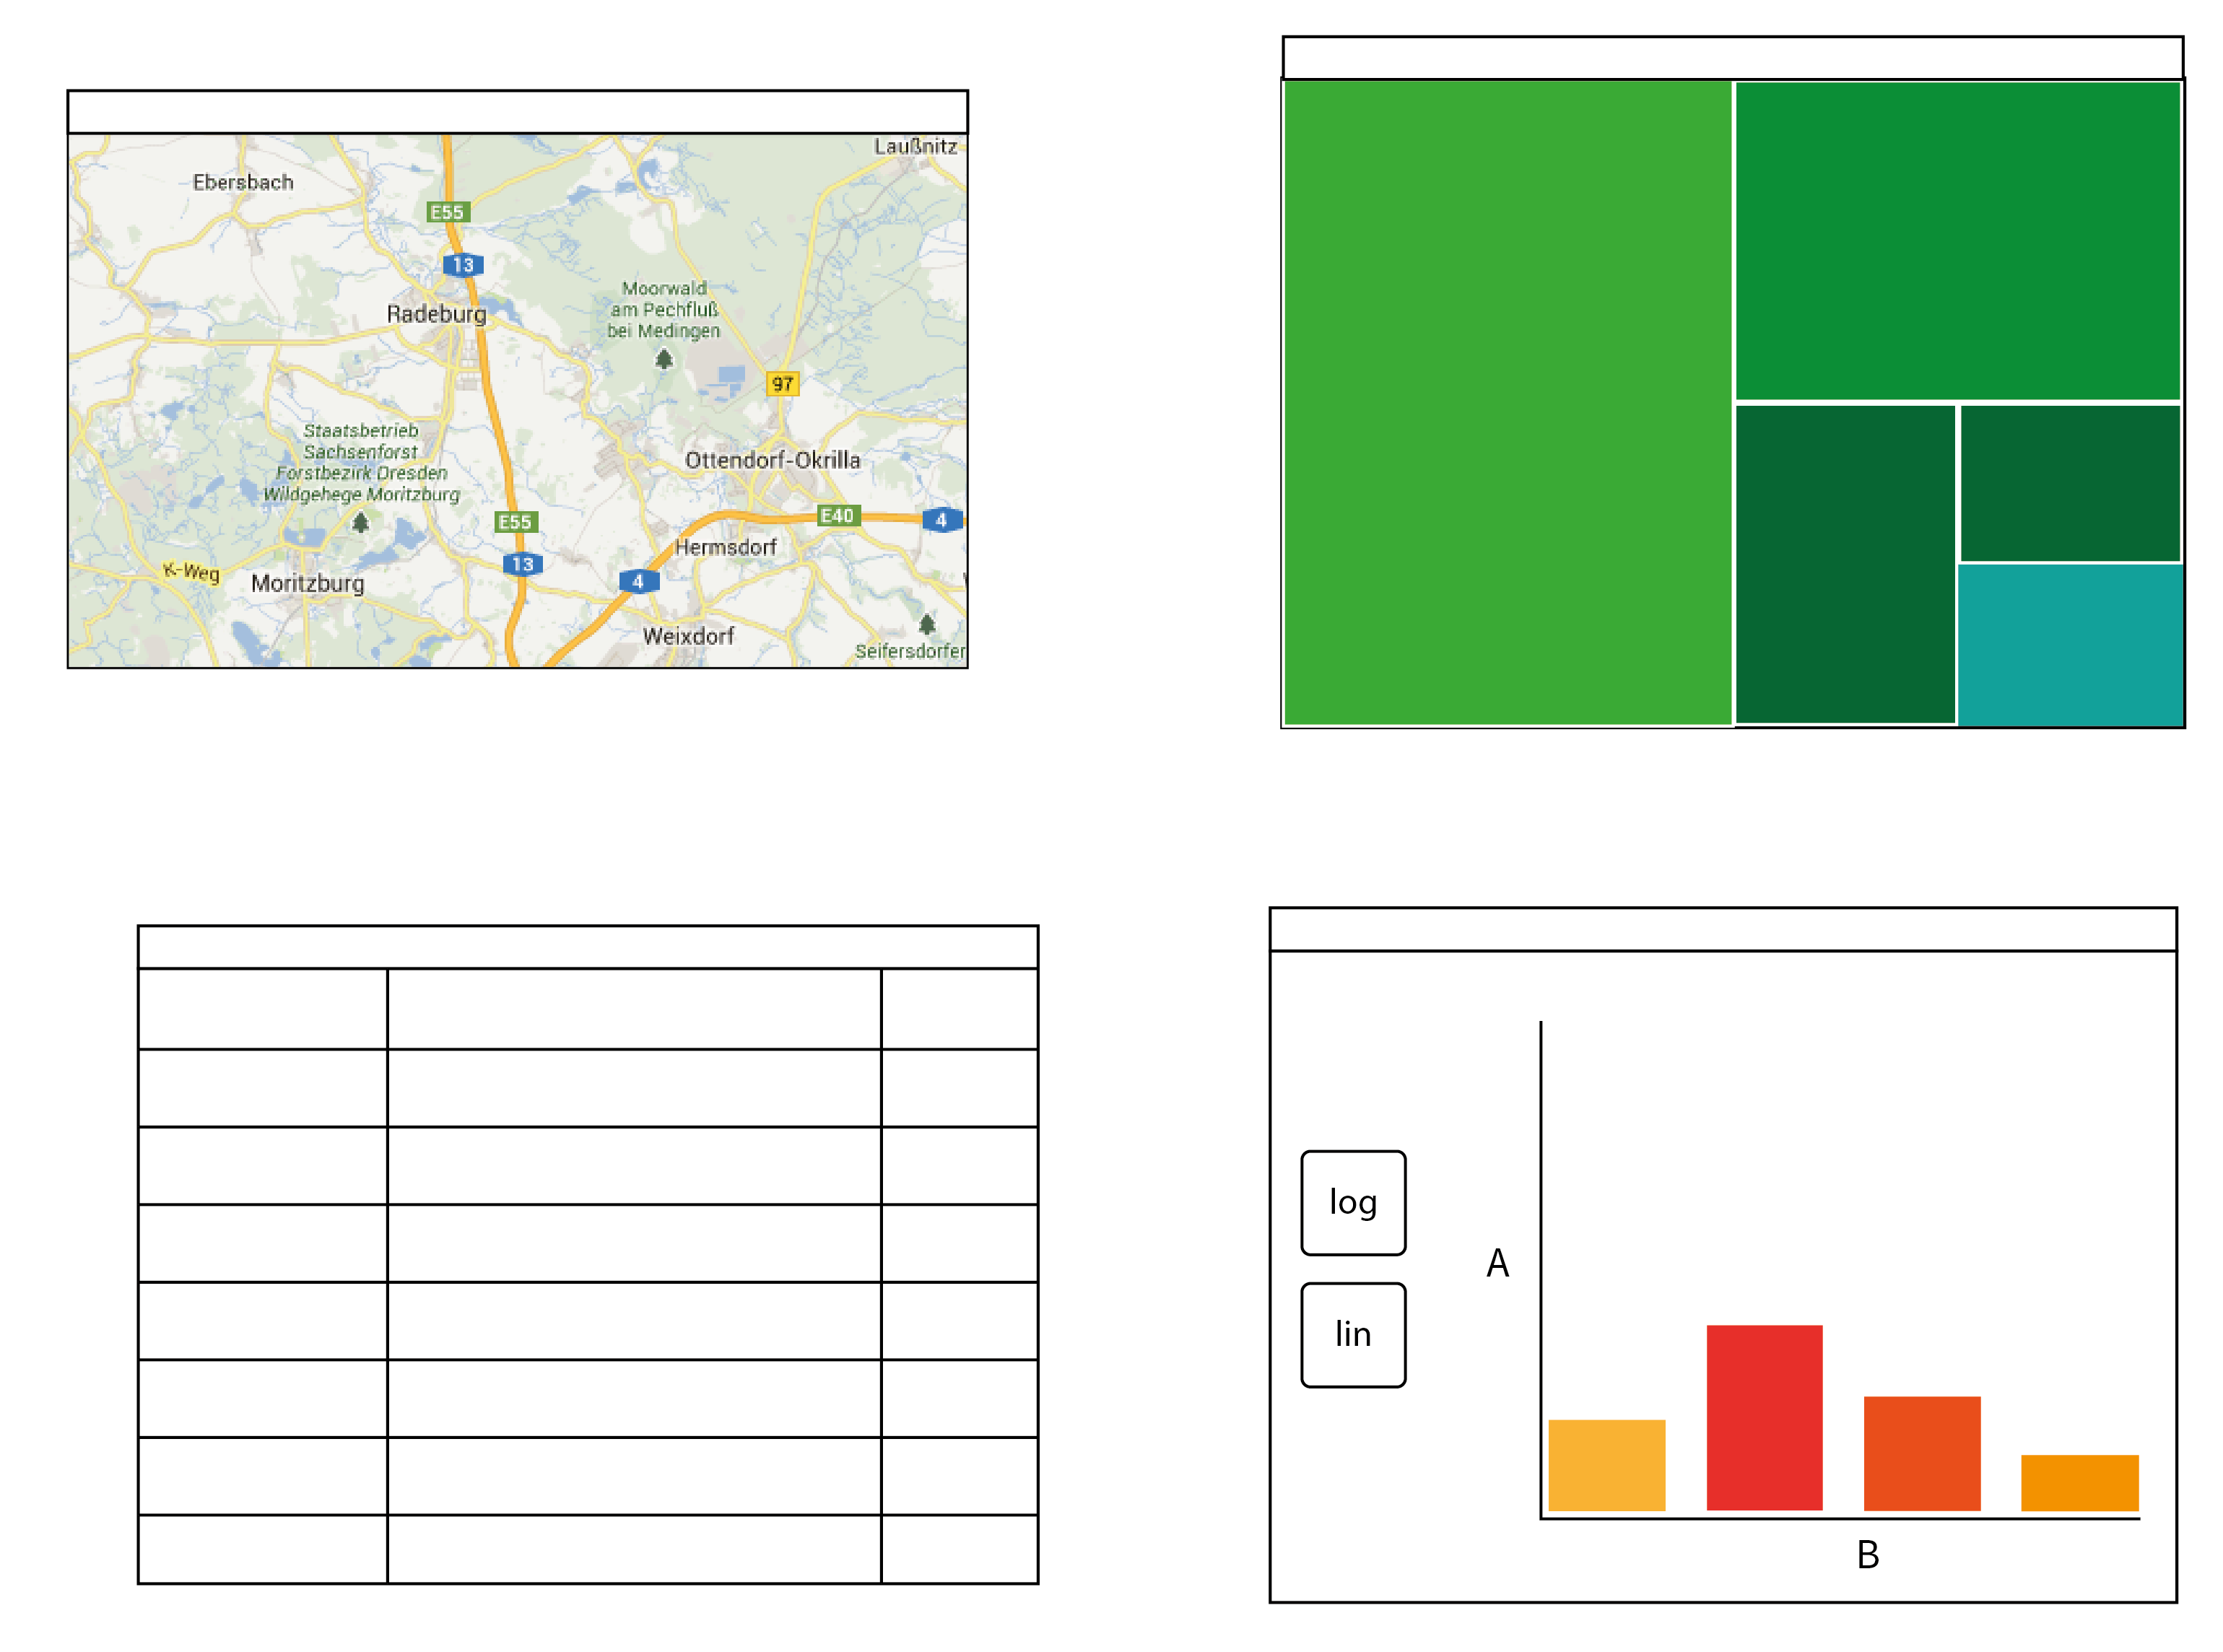
\includegraphics[width=0.5\textwidth]{images/konzeption-ui-grundlage.png}
   \caption{Grundlage der UI Mockups}
   \label{figure:ui-grundlage}
\end{figure}

\subsubsection{Aufruf}

% warum sind buttons in der titelleiste

Funktionen, die der Nutzer aus eigener Initiative nutzen kann und komponetenspezifisch sind (z.\,B. Kommentare), werden über Buttons in der Titelleiste der Komponente aufgerufen. Das Hilfesystem kann sie wegen des \enquote{Black Box} Prinzips nicht in der Komponente selbst platzieren. Zwar könnte man UI Elemente für die Hilfefunktionen im Komponenten-Markup vorsehen, aber durch die Nutzung der Titelleiste wird dem Entwickler Aufwand erspart. Die UI für die aufgerufene Hilfe kann auf folgende Arten geschlossen werden:

\begin{itemize}
	\item Klick auf den Button, der sie aufgerufen hat
	\item Klick auf den \enquote{Schließen}-Button oben rechts
\end{itemize}

\subsubsection{Art}

% wie sieht ui für dings grob aus?

Das User Interface für die ausgewählte Hilfefunktion wird links oder rechts der Komponente in einer Sidebar dargestellt (Abbildung~\ref{figure:ui-basics},~1). Gegenüber einem Popover (2) hat sie den Vorteil, dass sie sowohl links als auch rechts funktioniert. Ein Popover kann nur über der Titelleiste angezeigt werden, ansonsten werden große Teile der Komponente verdeckt (3). Die Sidebar kann in der Größe variieren (4), da für die Kommentare vermutlich mehr Platz benötigt wird als beispielsweise für die Reportingfunktion.

\begin{figure}[htbp]
   \centering
   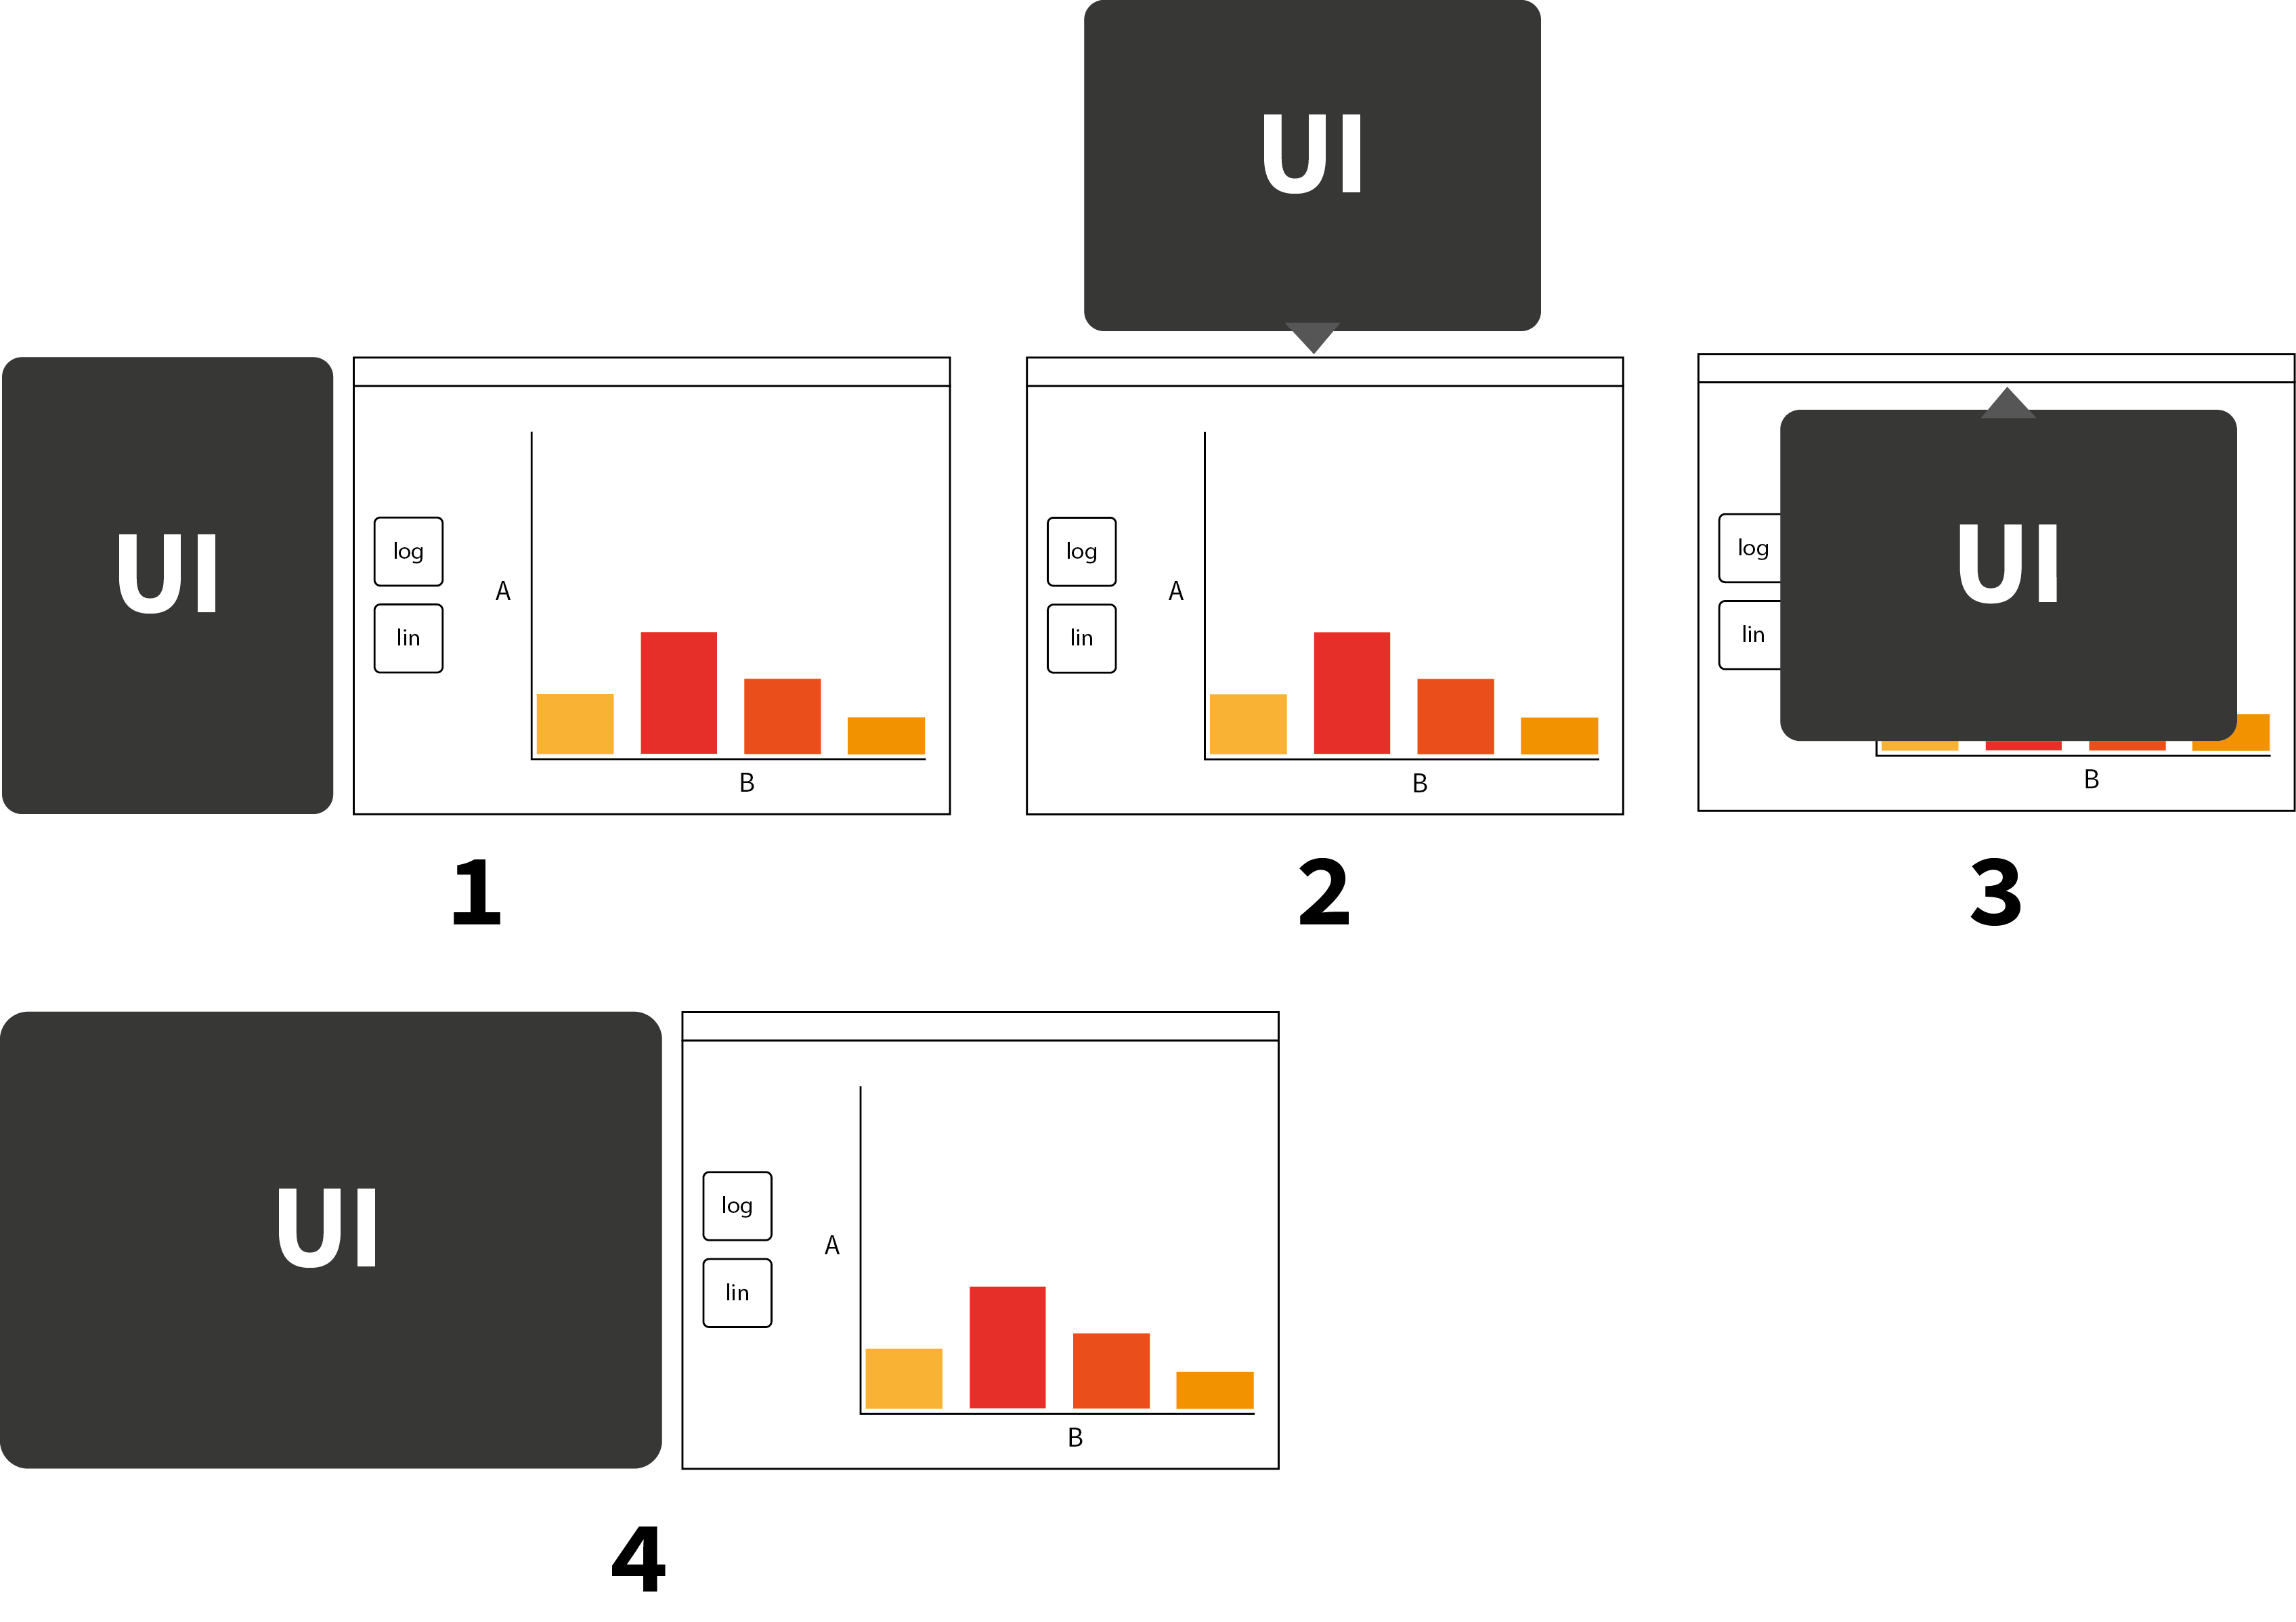
\includegraphics[width=0.5\textwidth]{images/konzeption-ui-basics.png}
   \caption{Verschiedene Möglichkeiten zur Platzierung der Hilfe UI}
   \label{figure:ui-basics}
\end{figure}

\subsubsection{Ort}

Dass die Sidebar mal links, mal rechts angezeigt wird, könnte beim Nutzer für Verwirrung sorgen. Jedoch scheint dieses Problem das kleinste zu sein, wenn man über die Alternativen nachdenkt.
Beispielsweise könnte das Hilfesystem die Buttons in einer eigenen Button-Sidebar platzieren. Allerdings erscheint dann in 50~\% der Fälle die UI Sidebar auf der anderen Seite, was noch verwirrender ist. Die Button-Sidebar jeweils auf der Seite zu rendern, wo auch die UI der Hilfe angezeigt werden wird, ist ebenfalls schwer vorstellbar. Erstens sind unterschiedliche User Interfaces unterschiedlich groß. Während das Reporting noch links gerendert werden könnte, könnten die Kommentare nur rechts genug Platz haben. Zweitens müsste der Nutzer jedes Mal erst die Buttons suchen, da sie abhängig von der Größe der Komponente und der Position linker oder rechter Hand sind. Das stellt nicht unerheblichen mentalen Aufwand dar.
Zuletzt wäre es möglich, die Button-Sidebar auf beiden Seiten der Komponente anzuzeigen und eine davon zu deaktivieren. Diese Variante unterscheidet sich aber nicht viel von der eben beschriebenen, da der Benutzer dann nicht die Buttons selbst, sondern aktivierte Buttons suchen muss.

\subsubsection{Optik}

Visuelle Konsistenz ist wichtig, damit der Benutzer Elemente gleichen Typs erkennen kann. Deswegen hat der Bereich, in der Hilfefunktionen angezeigt werden, abgerundete Ecken. So hebt sich die UI für Hilfe von der normalen UI der Komponente, welche spitze Ecken aufweist, ab. Aus demselben Grund wird für die Hilfe UI ein dunkler Hintegrund gewählt, da der Hintergrund von VizBoard weiß ist. Um etwas hervorzuheben, wird prinzipiell die Farbe Orange benutzt, da dies im bestehenden VizBoard Farbschema so festgelegt wurde. Eine Überlagerung der Komponente mit einem leichten Grau dient der Blickführung zu einem nicht überlagerten Element. Ist die Komponente hingegen mit einem tiefen Grau überlagert, signalisiert die dunkle Fläche eine \enquote{No Click Area}, wo keine Interaktionen ausgeführt werden können. 

Offensichtlich sind die gewählten visuellen Effekte nicht mehr so nützlich, wenn eine Komponente einen dunklen Hintergrund aufweist. Schwarz mit Dunkelgrau zu überlagern macht für das menschliche Auge nur wenig Unterschied. Deswegen werden in diesem Fall dieselben Effekte mit Weiß und Hellgrau verwendet.

% todo: wieder dafür sorgen, dass im text auch steht, was auf den bildern zu sehen ist

\section{Intro}
\label{section:konzeption:intro}

Aus dem Szenario (Abschnitt~\ref{section:standderforschung:szenario}) wurde deutlich, dass dem Endnutzer zuerst ein Überblick über die verschiedenen ausgewählten Komponenten gegeben werden muss. Dieser beinhaltet folgende Punkte.

% was kommt rein?

\begin{enumerate}
	\item Art der Visualisierung, z.\,B. \enquote{Balkendiagramm}
	\item Beschreibung der Visualisierung, z.\,B. \enquote{Ein Diagramm, das durch auf der x-Achse senkrecht stehende, nicht aneinander grenzende Rechtecke die Häufigkeitsverteilung einer diskreten Variable veranschaulicht.}
	\item Visuelle Mappings, z.\,B. BIP auf der y-Achse und Länder auf der x-Achse.
	\item Links zu Tutorials, Videos und Erklärungen
	\item Vor- und Nachteile der ausgewählten Visualisierung, z.\,B. \enquote{übersichtlich, wenn wenige Farben vorhanden sind}
\end{enumerate}

% abgrenzung zu "der dev macht das"
Eine Möglichkeit -- so ist die Beschreibung einer Komponente bereits umgesetzt -- ist den Komponentenentwickler selbst einen Text dazu schreiben zu lassen. Er fügt diesen in die Komponentenbeschreibung ein, von wo das Hilfesystem ihn dann auslesen kann. Allerdings kann auf diese Weise kein einheitliches Vokabular bezüglich Informationsvisualisierungen sichergestellt werden. Ein einheitliches Vokabular ist aber wichtig, da unterschiedliche Bezeichnungen derselben Konzepte kontraproduktiv für das Verständnis sind. Deswegen werden die Informationen direkt zu den entsprechenden Konzepten in der VISO hinzugefügt. Von dieser zentralen Stelle kann das Hilfesystem sie dann auslesen und anzeigen, sodass die verwendeten Vokabeln konsistent bleiben.

% was bleibt draußen?

% links zu externen quellen
Nach Grammel \cite{Grammel2012} können Links zu Tutorials und Erklärungen hilfreich sein, Endnutzern Visualisierungen zu erklären. Da externe Quellen aber nicht durch das Hilfesystem kontrolliert werden, kann es nicht sicherstellen, dass überall ein einheitliches Vokabular benutzt wird. Wie bereits erwähnt ist ein konsistentes Vokabular wichtig für effektive Hilfestellungen, weswegen dieser Punkt in dieser Form nicht umgesetzt werden kann. Was allerdings möglich ist, sind vom VizBoard-Betreiber erstellte Tutorialvideos in Form von vertonten Animationen, die Aufbau und Vor- bzw. Nachteile grafischer Repräsentationen erklären. Das sind zwar viele Videos, aber die Anzahl der Repräsentationen ist endlich und nicht alle gleich wichtig\footnote{Ein Balkendiagramm ist gängiger und deswegen leichter verständlich als eine Scatterplot Matrix.}, weswegen der nötige Aufwand gerechtfertigt scheint.

% vor- und nachteile
Grammel schreibt ebenfalls, dass InfoVis-Novizen die Vor- und Nachteile von verschiedenen Visualisierungstypen und visuellen Mappings lernen sollten \cite[S. 125]{Grammel2012}. Es wäre möglich, allgemeine Eigenschaften von grafischen Repräsentationen in der VISO zu beschreiben. Diese sind abhängig von den dargestellten Daten und den visuellen Mappings. Die Eigenschaft \enquote{Übersichtlichkeit} ist bei einem Balkendiagramm mit drei Balken gegeben (Vorteil), bei 15 Balken nicht (Nachteil). Ähnlich verhält es sich mit der Farbkodierung: Ein Mensch kann bis zu acht Farben in einer Visualisierung gut unterscheiden (Vorteil) \cite{Mazza2009}, aber mehr nicht (Nachteil). Das Hilfesystem müsste dem Benutzer demnach sowohl die unterschiedlichen Vor- und Nachteile als auch deren Bedingungen präsentieren, was sehr viel Information für eine Einführung darstellt. Im schlechtesten Fall kann der Benutzer auch keinen Bezug zur konkreten Visualisierung herstellen, weil keine der aufgeführten Bedingungen erfüllt ist. Er kann die aufgestellte Hypothese nicht am Beispiel überprüfen, was laut Grundlagen schlecht für seinen Verständnisprozess ist (Abschnitt~\ref{section:standderforschung:grundlagen:user_assistance:sensemaking}). Hinzu kommt, dass diese Erklärung einen Schritt früher im VizBoard Workflow konzeptionell mehr Sinn macht. Dort wählt der Benutzer -- von VizBoard unterstützt -- die visuellen Mappings aus.

Aus den eben aufgeführten Gründen zeigt das Intro für eine Komponente folgende Informationen:

\begin{itemize}
	\item Art der Visualisierung
	\item Beschreibung
	\item Visuelle Mappings
	\item Tutorialvideo, wenn vorhanden
\end{itemize}

% interaktionshilfen - kommen später

Über die Interaktion mit der Visualisierung wird hier noch keine Aussage gemacht, da sie sehr umfangreich sein kann und den Rahmen des Intros sprengen würde. In Abschnitt~\ref{section:konzeption:bedienung} wird eine Hilfestellung zur Bedienung einer Komponente erarbeitet.

\subsection{User Interface und Interaktion}
\label{section:konzeption:intro:ui}

Nachdem der Benutzer bei der Visualisierung angekommen ist und die Komponenten sieht, wird der gesamte Viewport abgedunkelt und eine Sidebar neben der ersten Komponente (von links oben nach rechts unten) eingeblendet (Abbildung~\ref{figure:ueberblick}). Dort sind die im vorigen Abschnitt erläuterten Informationen zu finden: Die Art der Visualisierung (\enquote{Karte}), darunter eine Beschreibung einer Karte, Informationen zu den dargestellten Daten und zuletzt ein Tutorialvideo, wenn vorhanden. Mit den Pfeilen links und rechts kann zwischen den Beschreibungen für verschiedene Komponenten gewechselt werden. Über die Meta-Hilfe (Abschnitt~\ref{section:konzeption:meta-hilfe}) kann das Intro wieder aufgerufen werden, wenn es geschlossen wurde.

\begin{figure}[htbp]
   \centering
   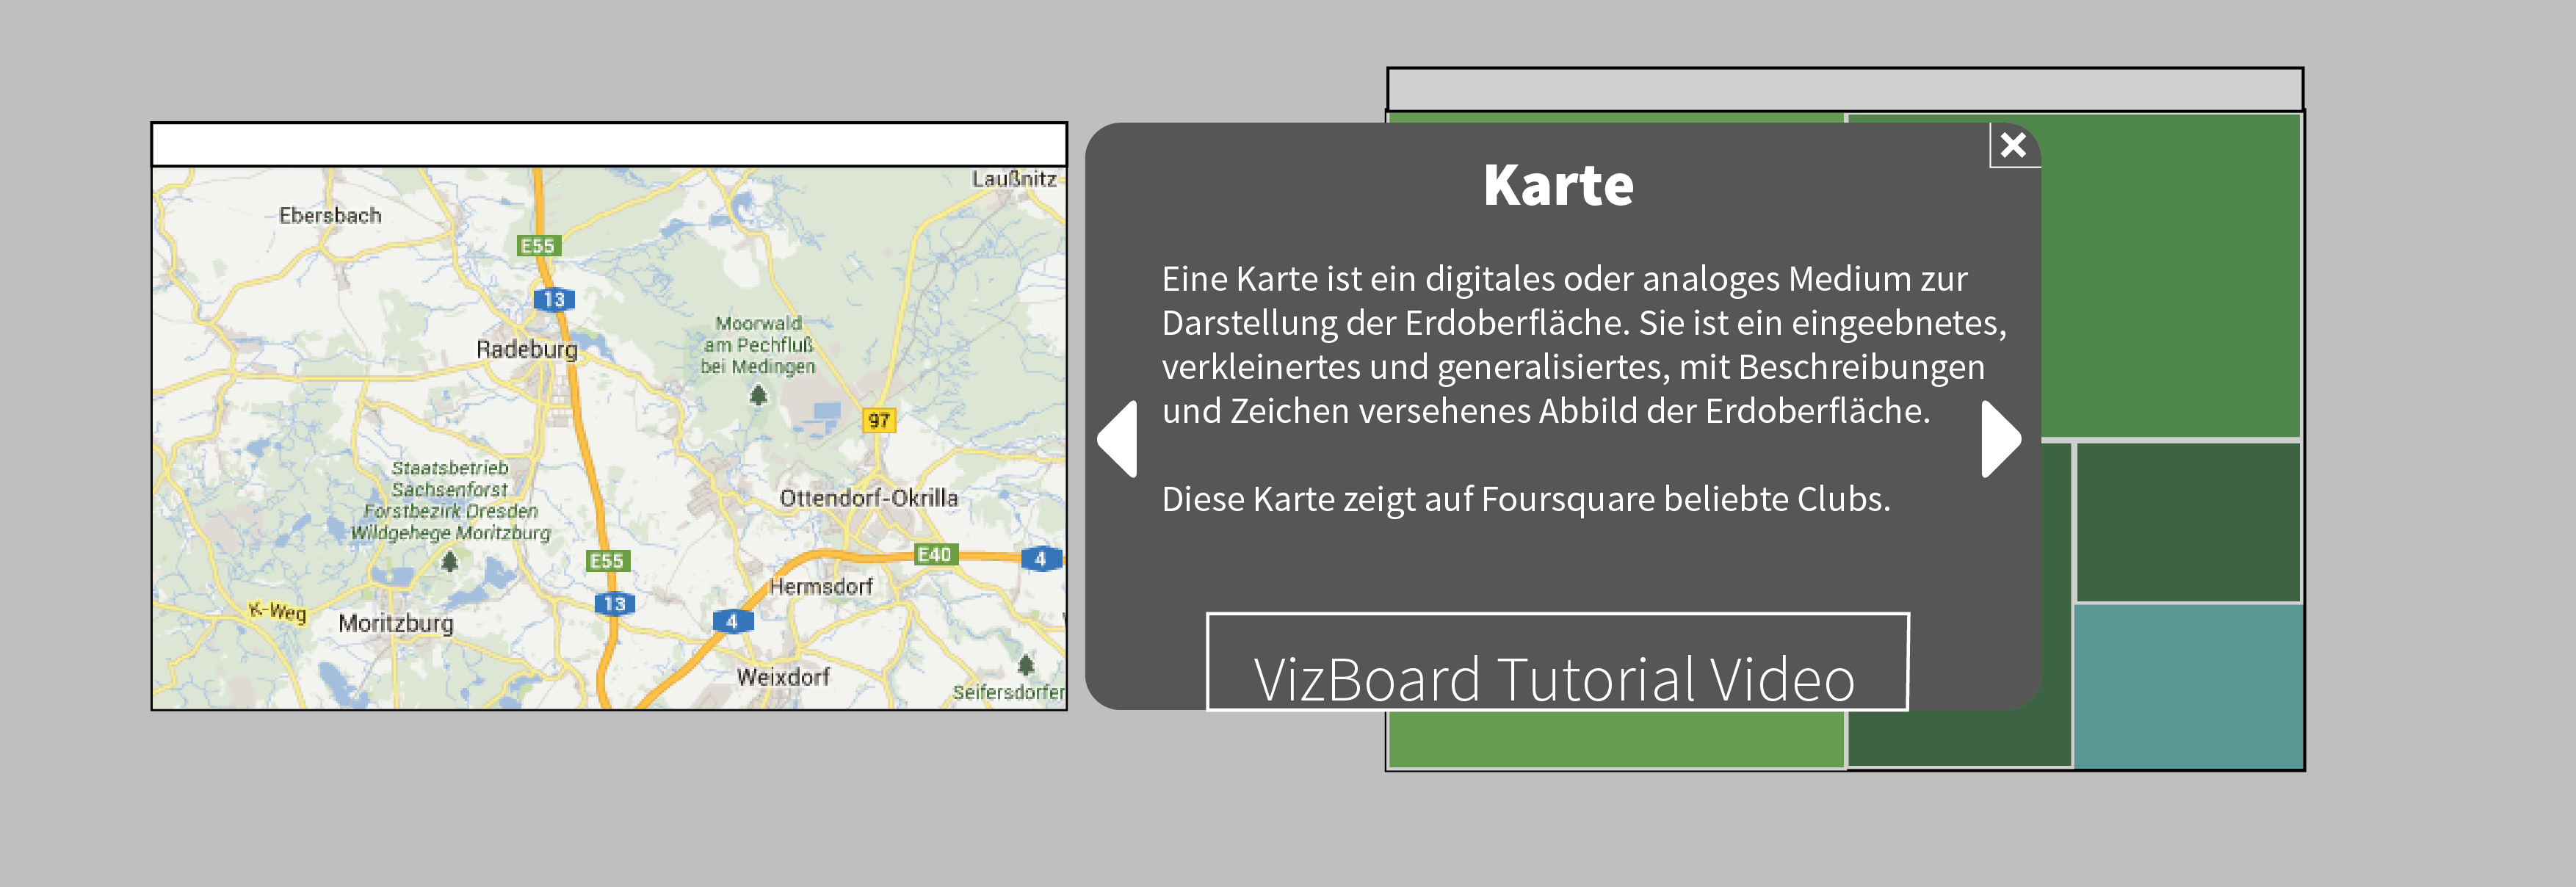
\includegraphics[width=0.75\textwidth]{images/konzeption-ueberblick.png}
   \caption{UI Mockup: Intro}
   \label{figure:ueberblick}
\end{figure}

\subsection{Backend}
\label{section:konzeption:intro:backend}

Die VISO (Abschnitt~\ref{section:standderforschung:grundlagen:cruise_vizboard:viso}) enthält bereits ein Vokabular für Informationsvisualisierungen. Deswegen ist es naheliegend, die Beschreibung der Visualisierung in die VISO hinzuzufügen. Die Art der grafischen Repräsentation muss der Komponentenentwickler in der Komponentenbeschreibung hinzufügen, dann kann das Hilfesystem die entsprechenden Daten auslesen. Der Inhalt der Visualisierung entspricht dem Domain Assignment, welches der Komponente von der Laufzeitumgebung mitgeschickt wird.

\section{Bedienung}
\label{section:konzeption:bedienung}

Da die Komponenten \enquote{Black Boxes} sind und von verschiedenen Entwicklern stammen, kann der Benutzer weder von verfügbaren möglichen Aktionen wie z.\,B. zoomen noch von einheitlicher Gestaltung der Interaktionen ausgehen. Beispielsweise wann eine Interaktion durch \texttt{MouseOver} anstatt \texttt{Click} ausgeführt wird. Deswegen ist eine Hilfestellung zur Bedienung notwendig.

% wieder erste möglichkeit: dev baut selbst hilfe ein. text+bilder: kein einfluss auf wortwahl, art der bilder, ausführlichkeit etc. Comics: für jede aktion eins, übelster aufwand, kann man nicht verlangen, außerdem 2. wer sagt dass ein prof. sw-entwickler das können soll?

Die einfachste Umsetzung der Hilfe zur Bedienung ist dem Komponentenentwickler eine Möglichkeit zu geben, Text und Bilder zu diesem Thema in die Komponentenbeschreibung einzufügen. Das hat allerdings den Nachteil, dass das Hilfesystem keinen Einfluss auf die Wortwahl, Gestaltung der Bilder oder Ausführlichkeit der Erklärung hat.

Hilfestellungen zur Bedienung würden vom Benutzer wahrscheinlich am besten verstanden, wenn sie tatsächlich vorhandene, konkrete Elemente der Komponente verwendete (\enquote{Semantic Transparency} \cite{Kohlhase2009}). Um zu demonstrieren, dass nach einem Klick die Tabelle sortiert sein wird, könnten die Zeilen derselben beispielhaft ihre Position wechseln. Assistance in dieser Form kann auf zwei Arten umgesetzt werden, die beide ihre Nachteile haben. Einerseits könnte eine Beschreibungssprache für Aktionen in der Komponentenbeschreibung angeben, welche Folgen eine Operation haben wird. So könnte das Hilfesystem selbst die Tabellenzeilen beispielhaft sortieren, da es nun weiß, wie der Vorgang \enquote{sortieren} aussieht. Der große Nachteil daran ist, dass es vermutlich immer einen Komponentenentwickler geben wird, der eine nicht vorgesehene Aktion in seiner Komponente umsetzen will und sie nicht beschreiben kann. Die zweite Lösung, eine semantisch transparente Assistance umzusetzen, ist den Komponentenentwickler für jede Aktion eine Methode in seiner Komponente hinzufügen zu lassen, die diese demonstriert. Zur Laufzeit würde die Methode einfach vom Hilfesystem aufgerufen. Das hat allerdings den Nachteil, dass dem Komponentenentwickler erheblicher Mehraufwand aufgebürdet wird und keine Einheitlichkeit der Assistance garantiert werden kann. Aus diesen Gründen ist eine andere Lösung notwendig.

Wie in den Grundlagen (Abschnitt~\ref{section:standderforschung:grundlagen:user_assistance}) gezeigt, können Comics eine effektive und attraktive Lösung für User Assistance sein. Allerdings stellt es für den Entwickler erheblichen Mehraufwand dar, für jede mögliche Aktion verschiedene Comicpanels zu erstellen. Davon abgesehen können (und sollen) die gestalterischen Fähigkeiten dazu nicht von ihm erwartet werden und das Problem der Kontrolle über den Inhalt ist auch nicht gelöst.

Aus diesem Grund werden die Comicpanels vom Hilfesystem automatisch erstellt. Es bleibt die Frage der Präsentation: Aus den Grundlagen geht hervor, dass eine multimodale Ausgabe (akustisch-verbal und visuell) zur Lerneffektivität beiträgt. Darauf wird aber aus zwei Gründen verzichtet. Einerseits sollen beide Kanäle gleichzeitig ausgegeben werden. Das ist problematisch, weil vier Panels darzustellen wesentlich schneller möglich ist als eine verbale Erklärung für den Vorgang zu sprechen. Die Darstellung der Panels müsste sich der Audioausgabe anpassen und würde wesentlich langsamer vonstatten gehen. Eine nichtfunktionale Anforderung an die Hilfestellung ist aber, dass der Benutzer die Hilfe schnell aufnehmen und verarbeiten können soll. Zweitens wird automatische Soundausgabe gemeinhin als schlechte Usability angesehen. Hauptsächlich weil der Nutzen von Screenreadern dadurch eingeschränkt wird, aber auch weil der Benutzer automatische Wiedergabe nicht kontrollieren kann und die Audiodaten Bandbreite beanspruchen.

% also bleibt es an uns hängen.

\subsection{API und Komponentenbeschreibung}
\label{section:konzeption:bedienung:api}

% ### daten sammeln

Die VISO enthält im Namensraum \texttt{viso:activity} Konzepte der hierarchischen Aktivitätstheorie nach Kuutti \cite{Kuutti1996}:

\begin{itemize}
	\item \textbf{Aktivitäten} stellen langfristige Ziele des Benutzers dar, die nicht unmittelbar zu Ergebnissen führen (müssen). In Bezug auf das Szenario (Abschnitt~\ref{section:standderforschung:szenario}) wäre die Aktivität von Anna \enquote{mehr über die geografische Verteilung verschiedener Genvariationen lernen}.
	\item \textbf{Aktionen} sind Teilziele der Aktivität. Im Szenario sind das \enquote{VizBoard aufrufen}, \enquote{Komponenten auswählen} etc.
	\item Aktionen bestehen wiederum aus einer Kette von \textbf{Operationen}, also beispielsweise Klicks oder Drags.
\end{itemize}

Für das Hilfesystem sind Operationen und Aktionen relevant, da Aktivitäten nicht beeinflusst werden können. Aktionen einer Komponente sind beispielsweise zoomen, suchen oder filtern; Operationen sind etwa Klicks, Drags oder Multitouch-Gesten.

Die Komponentenbeschreibung gibt bereits Auskunft über die verfügbaren Aktionen in einer Komponente (Capabilities). Es fehlen aber noch Informationen darüber, welche Operationen auf welchen Elementen die Aktion ausführen. Um dem beizukommen, werden Operationen aus der VISO (\enquote{welche Operationen}) zusammen mit CSS Selektoren (\enquote{welche Elemente}) in der Komponentenbeschreibung definiert. Äquivalente Operationen, die denselben Effekt haben, werden zusammengefasst. Zu einer Aktion (Capability) wird dann eine Liste von äquivalenten Operationen angegeben, wobei die Reihenfolge die notwendige Ausführungsreihenfolge darstellt. So können auch zusammengesetzte Operationen -- beispielsweise zuerst Menü aufrufen, dann sortieren -- abgebildet werden. Außerdem kann der Komponentenentwickler eine Anzahl von Sekunden definieren, die bei der Generierung der Panels gewartet werden soll. Das ist beispielsweise sinnvoll, wenn längere Animationen zu erwarten sind. Zusätzlich ist es möglich, dass der Entwickler Zusatzinformationen in Stichworten angibt. Zum Beispiel kann eine Tabelle durch unterschiedliche Elemente nach verschiedenen Spalten \enquote{sortiert} (Aktion) werden. Dabei ist es wichtig zu wissen, welches Element nach welcher Spalte sortiert. Die erwähnten Zusätze zur Komponentenbeschreibung sollten allerdings optional sein, falls der Komponentenentwickler keine Hilfe für bestimmte Aktionen anbieten will.

\subsection{Generierung der Assistance}
\label{section:konzeption:bedienung:generierung}

% ### assistance generieren

% warum müssen wir bilder generieren und wie sehen die aus?

Die User Assistance zur Bedienung soll ein Comic werden, der per Definition wiederum aus mehreren Panels besteht, die Bilder und/oder Text enthalten \cite{McCloud1994}. Die Bilder der Panels können nicht a priori gezeichnet werden, da der Inhalt der Komponenten unbekannt ist (\enquote{Black Box} Prinzip). Aus diesem Grund müssen sie automatisch generiert werden. Die einfachste Möglichkeit dafür sind Screenshots der Komponente.

% wie machen wir das?

Dazu wird ein sogenannter \enquote{Headless Browser} verwendet. Das ist ein programmierbarer Browser ohne grafische Benutzeroberfläche, der z.\,B. Screenshots einer Seite abspeichern oder Testskripte ausführen kann. Beispiele sind unter anderem PhantomJS\footnote{\url{http://phantomjs.org/}}, HTMLUnit\footnote{\url{http://htmlunit.sourceforge.net/}} oder Ghost\footnote{\url{http://jeanphix.me/Ghost.py/}}.

% wie läuft das ab?

Bei der Generierung der Panels ist zuerst das Component Repository beteiligt. Sobald eine Komponente hinzugefügt oder upgedatet wurde, parst das CoRe die entsprechende Komponentenbeschreibung und schickt eine Anfrage an den Hilfeservice. Dieser kann ins CoRe integriert sein, sollte dem \enquote{Separation of Concerns} Designprinzip folgend aber davon getrennt sein, da es schon für Matching, Ranking und Verwaltung der Komponenten zuständig ist. Der Hilfeservice rendert die Komponente mit Hilfe des Headless Browsers in einer CRUISe Testumgebung. Sie besteht aus folgenden Komponenten:

% todo cruise testumgebung, was gehört da alles rein?

\begin{itemize}
	\item Laufzeitumgebung: Sie ist unter anderem für die Initialisierung und das Layout der Komponenten nötig.
	\item Data Repository: Die Komponente muss Daten darstellen, welche aus dem DaRe kommen können.
	\item Component Repository: Das CoRe ist für die Verwaltung der Komponenten zuständig und stellt u.\,a. die Komponentenbeschreibungen bereit. Diese sind notwendig um die Operationen und Aktionen auslesen zu können.
\end{itemize}

Es wurde eben erklärt, dass das DaRe die (Test-)Daten für eine Komponente liefern kann. Der Komponentenentwickler gibt in der Komponentenbeschreibung den gewünschten Datensatz an, welcher bei der Generierung der Assistance geladen wird. Das kann ein \enquote{echter} Datensatz oder ein vom VizBoard-Betreiber zur Verfügung gestellter Testdatensatz sein. Es kann allerdings passieren, dass das DaRe keine passenden Daten enthält, weil die Komponente sehr spezielle Daten visualisiert (z.\,B. 3-Sterne-Hotels in Andorra). Dann sollte der Komponentenentwickler zusammen mit der Komponente Testdaten hochladen können oder eine URL angeben, unter der sie zu finden sind. Das ist zwar etwas Mehraufwand, aber es kann angenommen werden, dass im Laufe der Entwicklung einer Komponente sowieso Testdaten verwendet wurden. Sie müssen in den meisten Fällen also nicht mehr erstellt, sondern nur noch hochgeladen werden.

Nachdem die Komponente vom Hilfeservice gerendert wurde, führt er folgende Schritte aus:

\begin{enumerate}
	\item Erstelle einen Screenshot vom Ausgangszustand der Komponente
	\item Für jede verfügbare Aktion:
	\begin{enumerate}
		%\item Finde die Bounding Box der relevanten Elemente
		\item Für jede Liste von äquivalenten Operationen:
		\begin{enumerate}
			\item Für jede Operation:
			\begin{itemize}
				\item Finde die Bounding Box der betroffenen Elemente und speichere sie
				\item Hebe betroffene Elemente hervor
				\item Erstelle einen Screenshot der Komponente
				\item Setze Zustand der betroffenen Elemente zurück
			\end{itemize}
		\end{enumerate}
		\item Führe Aktion aus
		\item Warte die definierte Anzahl an Sekunden
		\item Erstelle einen Screenshot vom Ergebnis der Aktion
	\end{enumerate}
\end{enumerate}

% hell und dunkel unterscheiden

Nachdem alle nötigen Screenshots der Komponente erstellt wurden, muss das Hilfesystem eine Kategorisierung in \enquote{helle Komponente} und \enquote{dunkle Komponente} vornehmen. Das ist nötig, damit das Hilfesystem zur Laufzeit weiß, ob es dunkle oder helle visuelle Effekte einblenden soll. Eine naive Möglichkeit dazu wäre mit Hilfe einer Bildverarbeitungsbibliothek wie OpenCV\footnote{\url{http://opencv.willowgarage.com/wiki/}} die Screenshots zu binärisieren, also in Bilder aus schwarzen und weißen Pixeln umzuwandeln. Enthält die Mehrzahl der Bilder mehr schwarze als weiße Pixel, wird die Komponente als \enquote{dunkel} eingestuft, ansonsten als \enquote{hell}.

% todo anbieten der assistance diskutieren: bilder in smcdl einbinden, eigener webservice, core.
Die Bilder der Comics können auf unterschiedliche Weise ans Hilfesystem ausgeliefert werden. Eine Möglichkeit ist die Bilder nach Generierung in der Komponentenbeschreibung zu definieren, so wie es bereits mit einem Screenshot der Komponente gemacht wird. Ebenso könnte ein Webservice die Bilder über eine REST API anbieten, von wo das Hilfesystem sie zur Laufzeit lädt. Dieser Webservice kann eigenständig oder im CoRe integriert sein. \textbf{Fazit?}

\subsubsection{Einschränkungen}
\label{section:konzeption:bedienung:generierung:einschraenkungen}

% nachteile

Die vorgestellte Lösung hat auch Nachteile. Zunächst ist sie vom Document Object Model (DOM) abhängig, was eine automatische Hilfegenerierung für Komponenten ausschließt, die auf Flash, Silverlight oder ähnlichen Technologien basieren. Der Trend geht aber ohnehin zu HTML/SVG-basierten Visualisierungen (z.\,B. mit D3 \cite{Bostock2011} oder Raphaël\footnote{\url{http://raphaeljs.com/}}): Flash ist laut Adobe hauptsächlich für Videoauslieferung und Spiele gedacht \cite{Adobe2013} und Microsoft zieht HTML5 Silverlight vor \cite{Foley2010}. Deswegen sollte dieser Nachteil nicht ins Gewicht fallen.

Eine weitere Einschränkung ist, dass zeitabhängige Interaktionen wie zum Beispiel \enquote{MouseOver für 3 Sekunden} nicht modelliert werden können. Diese sind im Web aber ohnehin eher unüblich und werden als schlechte Usability betrachtet, weil sie nicht sichtbar und deswegen schwer zu entdecken sind.

\subsection{User Interface und Interaktion}
\label{section:konzeption:bedienung:ui}

% ### assistance anbieten

Die Hilfestellung zur Bedienung wird über einen ?-Button aufgerufen, den der Benutzer vielleicht von nativen Desktop-Applikationen kennt (Abbildung~\ref{figure:bedienung-step1}). Der Viewport der Komponente wird abgedunkelt und nur die Elemente, für die auch Hilfestellungen existieren, bleiben sichtbar. Neben der Komponente erscheint eine Sidebar, welche die verfügbaren Aktionen noch einmal auflistet. Die Assistance wird entweder nach einem Klick auf ein sichtbares UI Element oder ein Element der Liste aufgerufen. So kann der Benutzer sowohl die Frage \enquote{Was macht dieser Button?} als auch \enquote{Wie kann ich Aktion XY ausführen?} beantworten.

\begin{figure}[htbp]
   \centering
   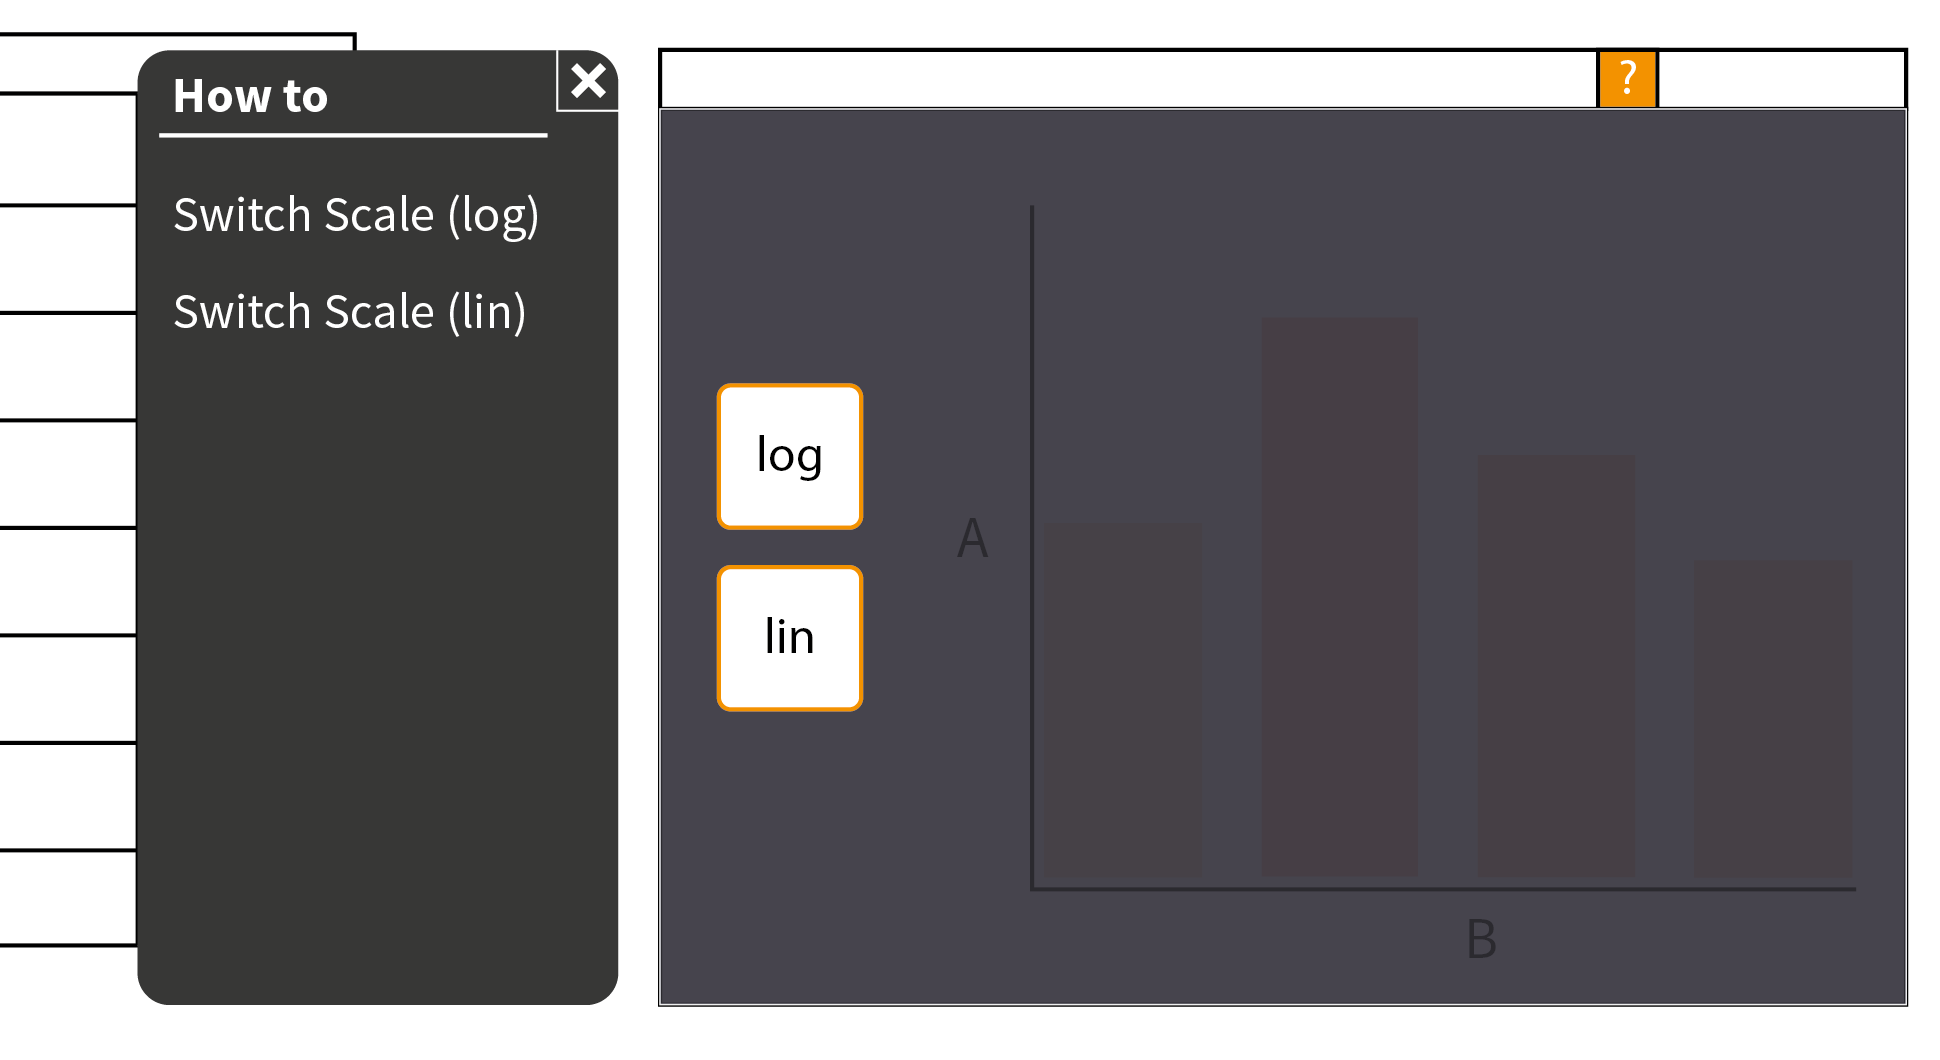
\includegraphics[width=0.5\textwidth]{images/konzeption-bedienung-step1.png}
   \caption{UI Mockup: Bedienung (Schritt~1)}
   \label{figure:bedienung-step1}
\end{figure}

Danach werden schrittweise mindestens vier Panels in der Komponente angezeigt (Abbildung~\ref{figure:bedienung-step2}). Der Inhalt der Panels ist in Abbildung~\ref{figure:bedienung-comic} zu sehen. Das erste Panel zeigt die ganze Komponente. Das zweite Panel startet mit dem gleichen Inhalt wie Panel~1, zoomt dann aber auf die relevanten UI Elemente. Panel~3 startet wiederum mit dem Inhalt von Panel~2, überblendet dann aber eine notwendige Operation. Das vierte Panel startet ebenfalls mit dem Inhalt aus Panel~2, zoomt aber auf eine Gesamtansicht wie in Panel~1 hinaus, sodass der Benutzer den Unterschied sehen kann. Mit den Pfeilen kann zwischen verschiedenen Operationen gewechselt werden, die dieselbe Aktion ausführen. Sollte eine Aktion aus mehreren zusammenhängenden Operationen bestehen, wiederholen sich die Panels~2 und~3 demensprechend.

\begin{figure}[htbp]
   \centering
   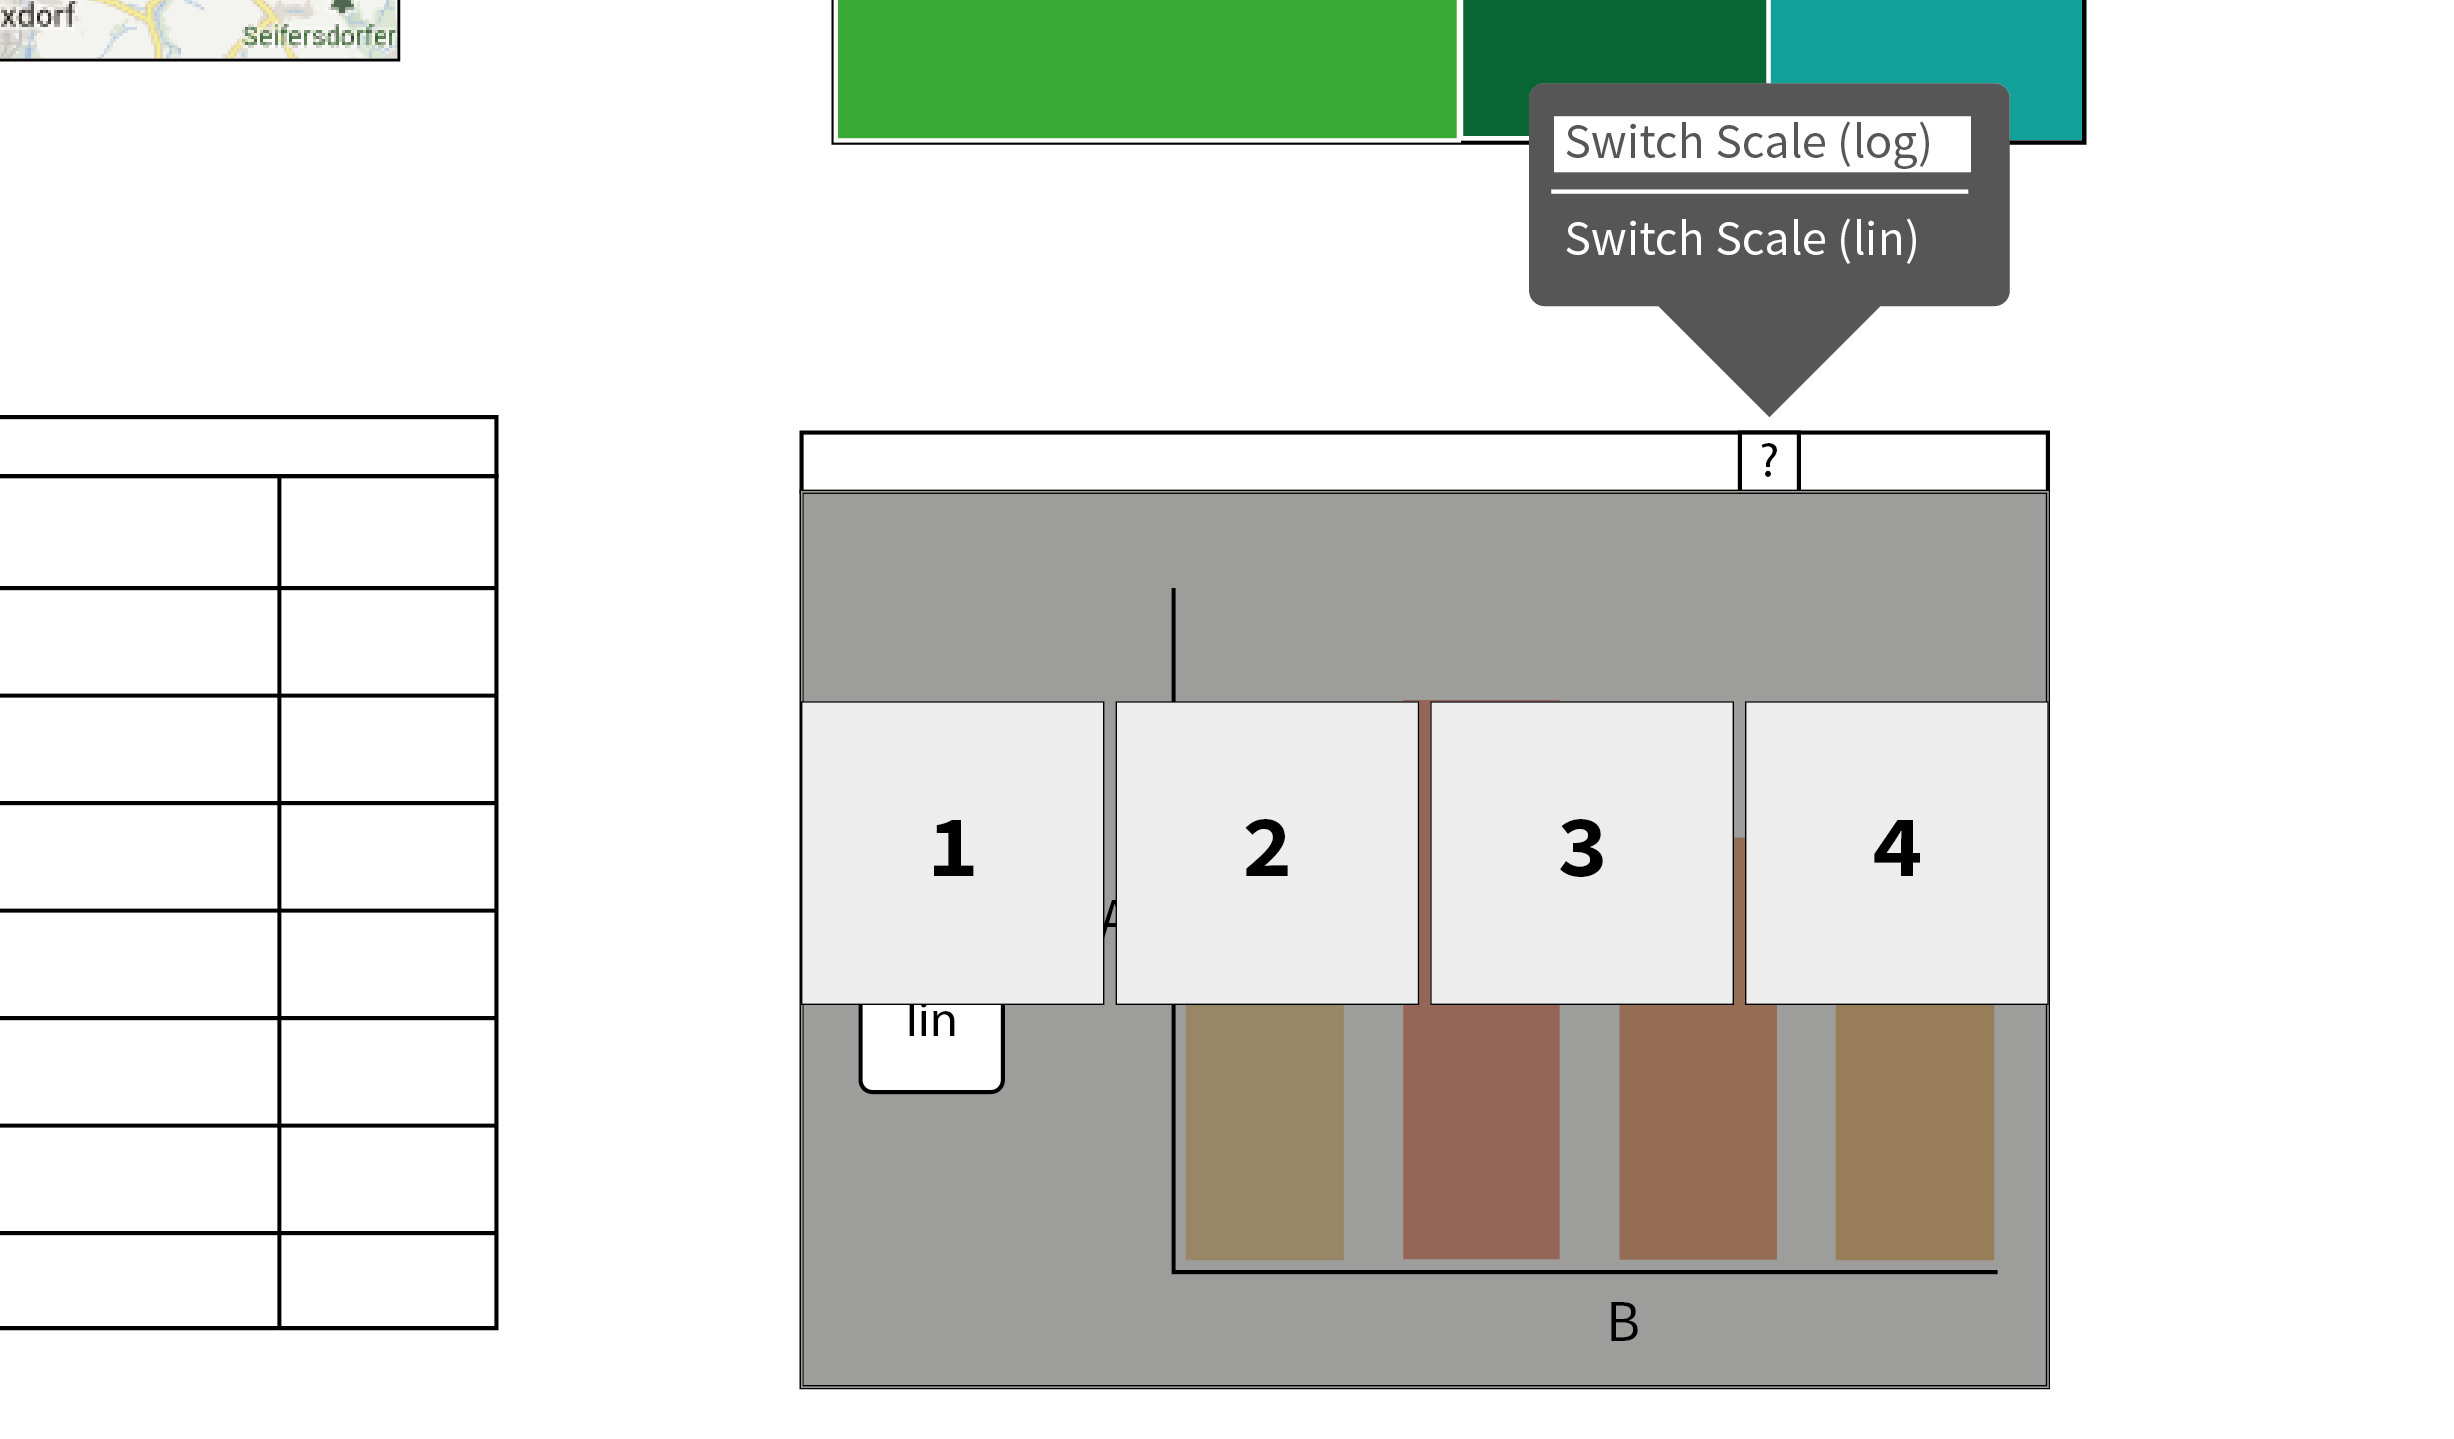
\includegraphics[width=0.5\textwidth]{images/konzeption-bedienung-step2.png}
   \caption{UI Mockup: Bedienung (Schritt~2)}
   \label{figure:bedienung-step2}
\end{figure}

\begin{figure}[htbp]
   \centering
   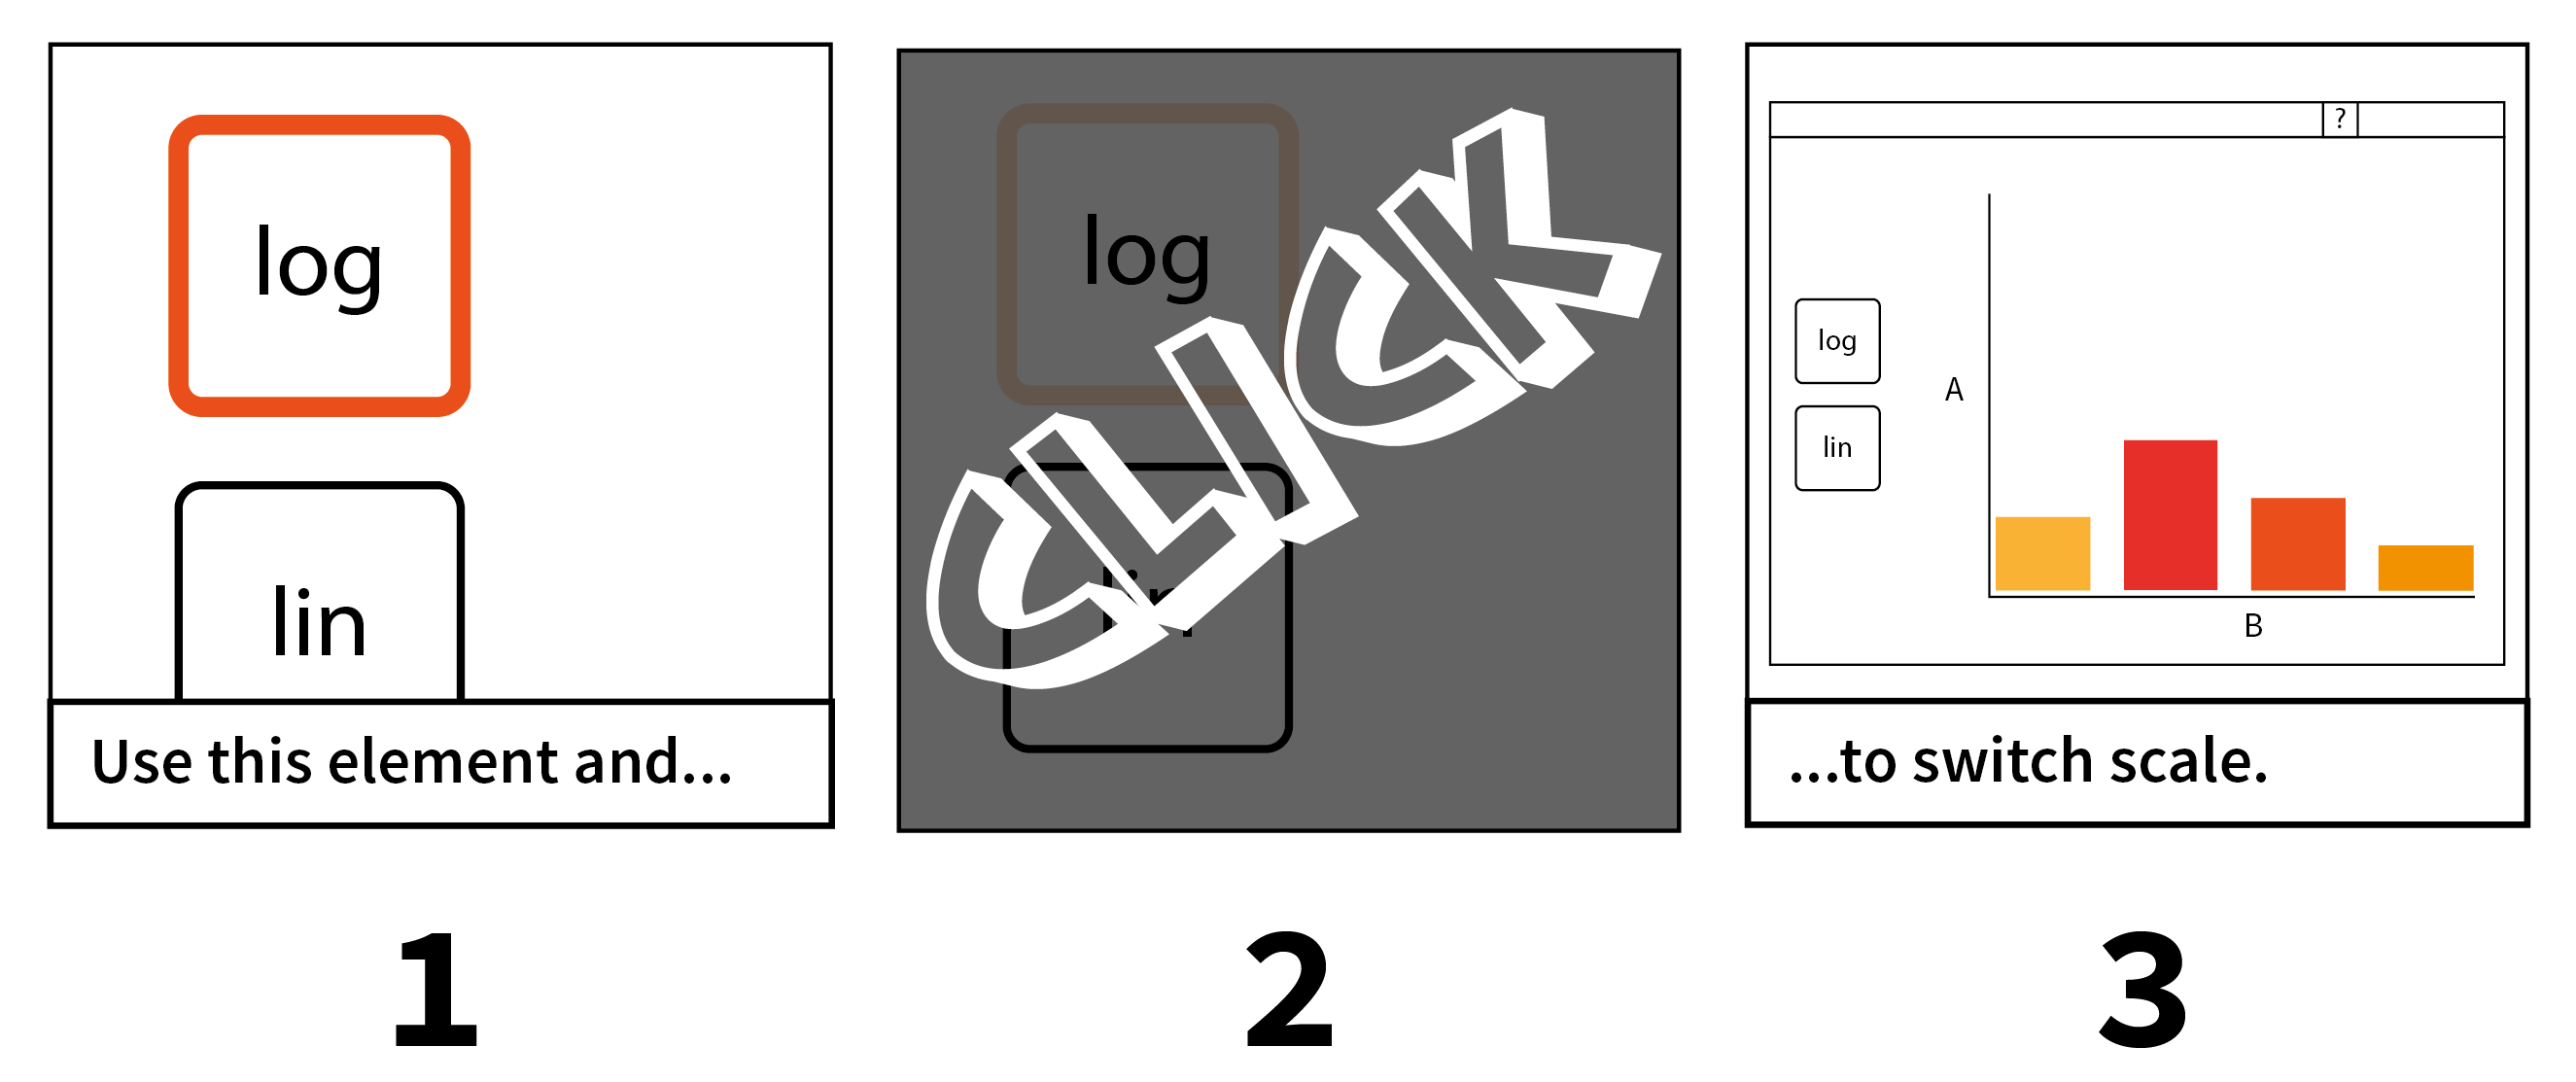
\includegraphics[width=0.75\textwidth]{images/konzeption-bedienung-comic.png}
   \caption{UI Mockup: Comic}
   \label{figure:bedienung-comic}
\end{figure}

Die Texte in den Panels werden zur Laufzeit hinzugefügt, da so beispielsweise auf die Sprache des Nutzers reagiert werden kann. Ansonsten müsste der Hilfeservice für jede unterstützte Sprache ein eigenes Bild erzeugen. Die dafür notwendigen Informationen sind:

\begin{itemize}
	\item Panel~1: Keine, Text wird zufällig aus einer Menge von Phrasen ausgewählt.
	\item Panel~2: Welche Elemente beteiligt sind.
	\item Panel~3: Name der Operation.
	\item Panel~4: Name der Aktion.
\end{itemize}

Diese werden aber schon im Schritt davor (Abbildung~\ref{figure:bedienung-step2}) benötigt, müssen also sowieso bekannt sein.

\section{Reporting}
\label{section:konzeption:reporting}

Wie bei jeder Software können bei den Komponenten in VizBoard Fehler auftreten. Externe APIs, die sie benutzen, wie zum Beispiel von Facebook oder Twitter können sich ändern. Visualisierte Daten können Fehler in der Komponente verursachen, beispielsweise durch nicht überprüfte \texttt{null} Werte oder wenn sie ein unerwartetes Format haben. Ebenso ist es möglich, dass VizBoard selbst Bugs enthält. Schlimmstenfalls fallen diese Fehler erst dem Endnutzer auf, welcher sie dann melden können soll.

Für diejenigen, die sich mit dem Bug Report befassen müssen -- also Komponentenentwickler bzw. VizBoard-Betreiber -- sind möglichst genaue Angaben sehr wichtig. Welcher Browser wurde benutzt? Welche Version? Welches Betriebssystem? Was genau hat nicht funktioniert? Ist der Fehler reproduzierbar? Wenn ja, wie? Diese und andere Fragen müssen beantwortet werden, um letzten Endes die Fehlerquelle zu finden. Also ob es an der Komponente liegt (z.\,B. wegen veralteten API Anfragen), an VizBoard (z.\,B. ein Bug im Event Broker) oder keinen der beiden (z.\,B. fehlerhafte Daten von der externen API). Aus Sicht des Endnutzers \enquote{funktioniert es nicht}, da er keine Kenntnisse der Programmierung besitzt und deswegen keine sinnvollen Hypothesen aufstellen, überprüfen und Schlußfolgerungen ziehen kann. Deswegen sollte der Endnutzer einen möglichst ausführlichen Text verfassen, um das Problem zu beschreiben, und die Möglichkeit haben, die Komponente prinzipiell als gut oder schlecht zu bewerten. Letztere Funktion existiert bereits in VizBoard und wird in die Reporting UI integriert. Die anderen Informationen, wie eben beispielsweise die Browserversion, sollten automatisch gesammelt und mitgeschickt werden.

\subsection{User Interface und Interaktion}
\label{section:konzeption:reporting:ui}

Der Nutzer klickt auf einen Button in der Titelleiste, beschreibt sein Problem und sendet ab (Abbildung~\ref{figure:reporting}). Optional kann er außerdem eine Bewertung abgeben.

\begin{figure}[htbp]
   \centering
   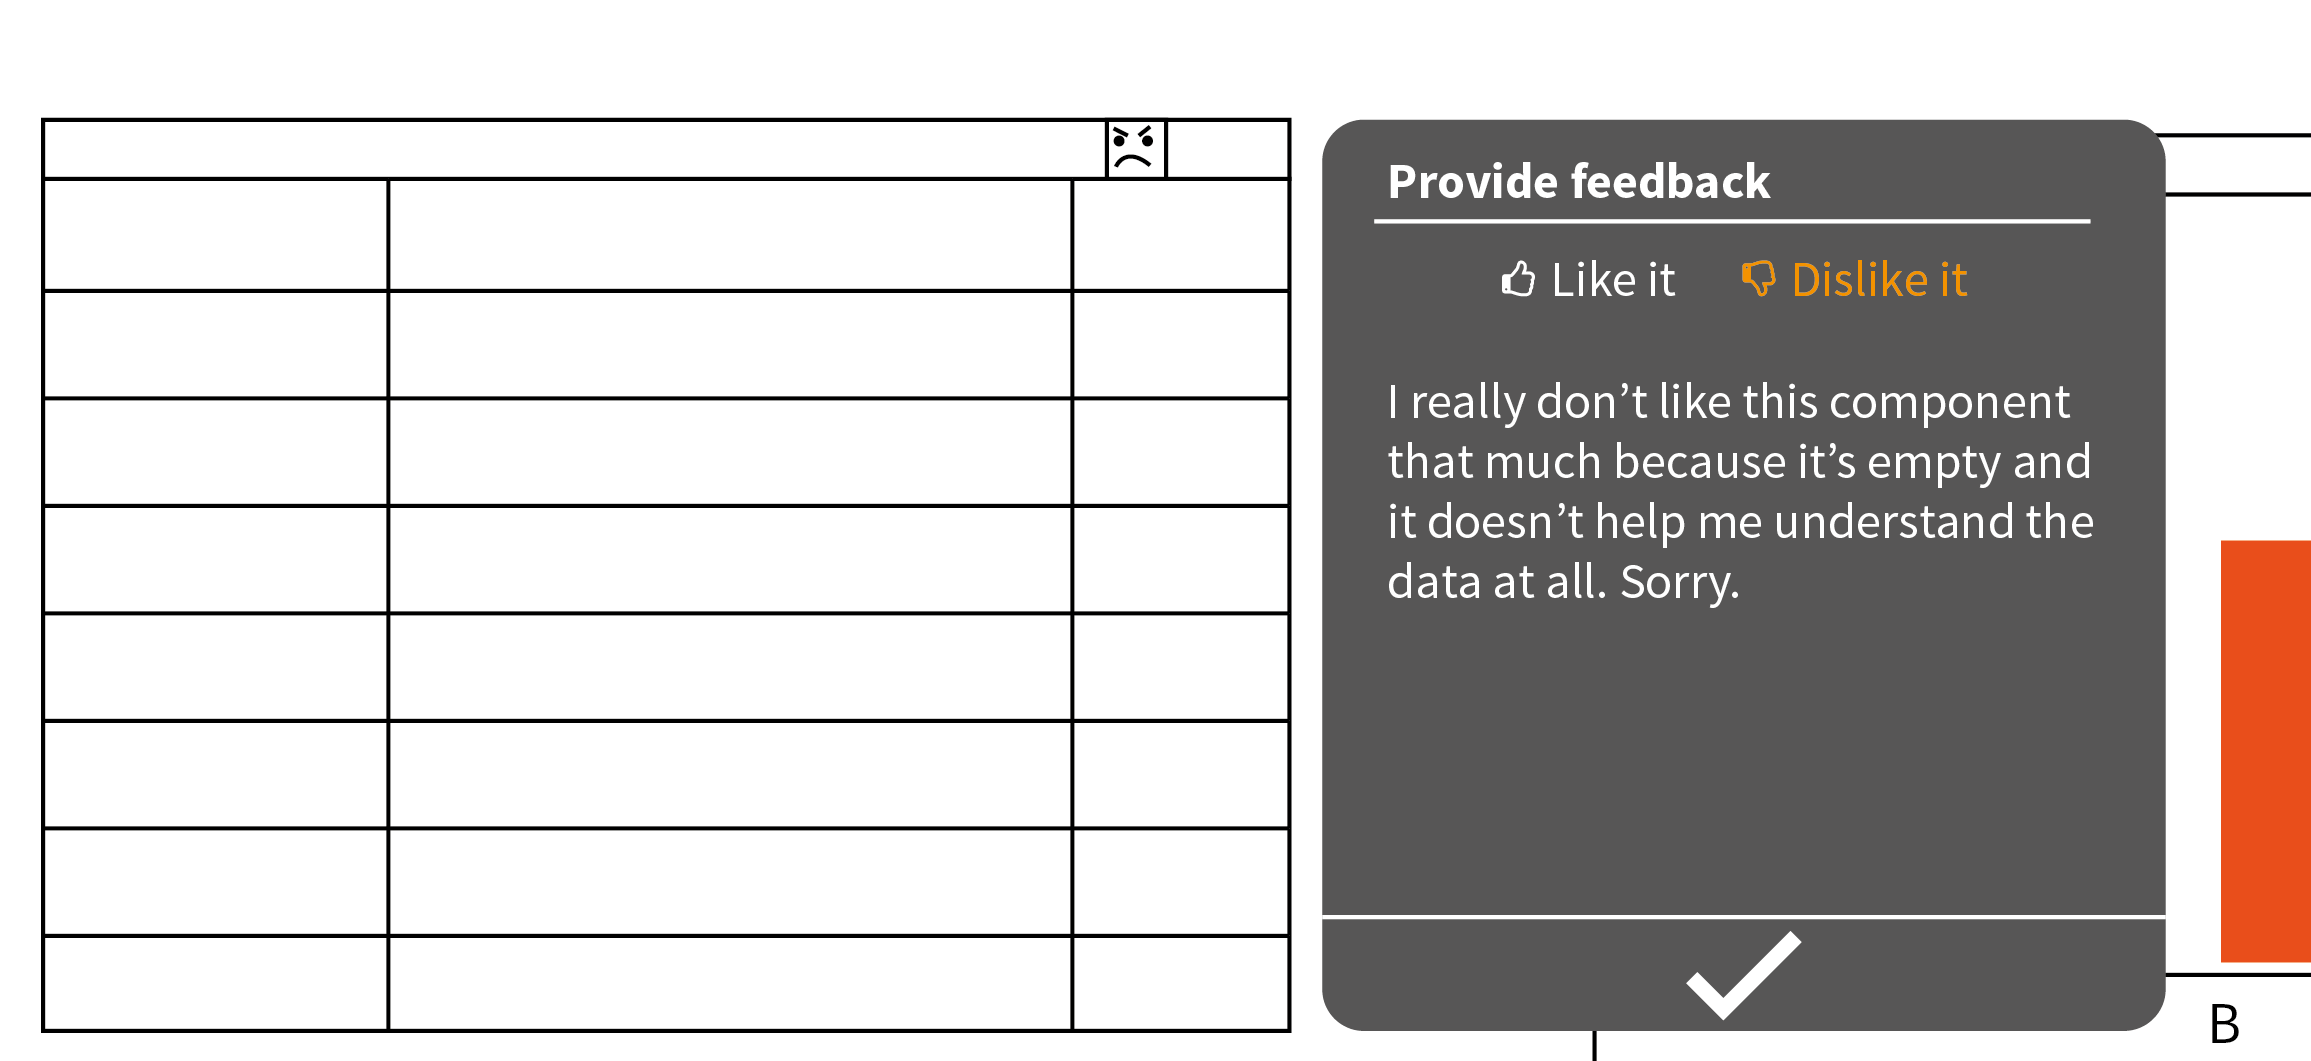
\includegraphics[width=0.5\textwidth]{images/konzeption-reporting.png}
   \caption{UI Mockup: Reporting-Funktion}
   \label{figure:reporting}
\end{figure}

\subsection{Backend}
\label{section:konzeption:reporting:backend}

% was kann man über javascript vom browser auslesen?
Informationen über den Browser befinden sich im DOM Objekt \texttt{window.navigator} und beinhalten unter anderem:

\begin{itemize}
	\item User Agent String, welcher Betriebssystem, Browser und deren Versionen enthält
	\item Sprache des Browsers
	\item Ob Cookies aktiviert sind
	\item Installierte Plugins, wie Java oder Flash
\end{itemize}

% was kann man über den context service bekommen?
% woher weiß man überhaupt, was es gibt? --> domänenspezifisches kontextmodell, ist also festgelegt.

Diese und andere notwendige Informationen können mit Javascript einfach ausgelesen werden. Noch mehr Informationen über den Nutzungskontext können über den Context Service (Abschnitt~\ref{section:standderforschung:grundlagen:cruise_vizboard}) bezogen werden. Dieser beinhaltet u.\,a. \textbf{WAS IST DA GENAU DRIN?}.

% noch sagen dass es denkbar wäre, das direkt an ein support system anzubinden

Die gesammelten Informationen über Nutzer, Browser und Anwendungskontext werden ans DaRe gesendet und dort abgespeichert. Das DaRe könnte aus der vom Nutzer abgegebenen Bewertung und Textklassifikation \cite{Sebastiani2002} in \enquote{positiv} oder \enquote{negativ} bestimmen, ob ein Ticket in einem Support System (wie z.\,B. OSTicket\footnote{\url{http://osticket.com/}}) des VizBoard-Betreibers erstellt werden soll. Die positiven Kommentare könnten beispielsweise für Testimonials auf der Startseite von VizBoard verwendet werden.

\section{Verlinkung}
\label{section:konzeption:verlinkung}

% einführung - warum brauchen wir verlinkung?

Es ist möglich, dass ein Benutzer in VizBoard auf vollständig (\enquote{Was ist ein Säurezeiger\footnote{Eine Pflanze, die nur auf Böden mit einem bestimmten ph-Wert wachsen kann.}?}) oder teilweise (\enquote{Wie ist das BIP definiert\footnote{Der Gesamtwert aller Waren und Dienstleistungen, die innerhalb eines Jahres in einer Volkswirtschaft hergestellt wurden und dem Endverbrauch dienen.}?}) unbekannte Begriffe trifft. Um das Verständnis der Daten zu fördern, müssen diese erklärt werden, weswegen sie mit einer externen Wissensbasis verlinkt sein sollen. Zu erklärende Begriffe werden vermutlich hauptsächlich in Legenden von Visualisierungen zu finden sein, können prinzipiell aber auch in Freitext vorkommen.

\subsection{Markup und Backend}
\label{section:konzeption:verlinkung:backend}

Um zu erklärende Begriffe für das Hilfesystem auffindbar zu machen, zeichnet der Komponentenentwickler sie mit einer dafür vorgesehenen CSS Klasse aus: Eine Klasse für Legenden, eine für Freitext. Diese können entweder in der Komponentenbeschreibung angegeben und so selbst gewählt werden, oder sie werden vom Vizboard-Betreiber festgelegt. Hier wird die letzte Variante umgesetzt, weil sie dem Komponentenentwickler etwas Aufwand erspart und \enquote{Kollisionen} mit bereits vorhandenen Klassen erstens unwahrscheinlich sind und zweitens einfach behoben werden können (beispielsweise mit dem Präfix \texttt{my-}). Der zu erklärende Begriff ist dann der Textinhalt des Tags mit der entsprechenden Klasse.

Auf diese Weise können die erklärungsbedürftigen Konzepte über CSS Selektoren gefunden werden. Betreffen die Begriffe Legenden der Visualisierung, ist das korrespondierende Konzept bereits in Form einer URL im Domain Assignment enthalten, welches die Laufzeitumgebung der Komponente mitteilt. Für frei gewählte Begriffe muss eine eigene Anfrage an das Data Repository gestellt werden, welches das entsprechende Konzept findet, eine Beschreibung lädt und zurück liefert. Dann kann es zusammen mit einem Link zu einer Erklärung angezeigt werden.

\textbf{Wie kommt die Beschreibung aus dem Domain Assignment, was nur eine URL zu DBpedia, Freebase oder irgendeine andere obskure Enzyklopädie ist (kein einheitliches Format!)? Vielleicht kann das DaRe die vorher schon fetchen und gleich mitgeben?}

\subsection{User Interface und Interaktion}

Hinter die entsprechend markierten DOM Elemente (siehe Abschnitt~\ref{section:konzeption:verlinkung:backend}) wird ein Fragezeichen eingefügt. Dieses kann angeklickt werden, woraufhin eine Sidebar mit einer kurzen Erklärung des Konzepts angezeigt wird (Abbildung~\ref{figure:verlinkung}). Sie enthält auch einen Link, der zu einer Erklärung in einer externen Wissensbasis führt.

\begin{figure}[htbp]
   \centering
   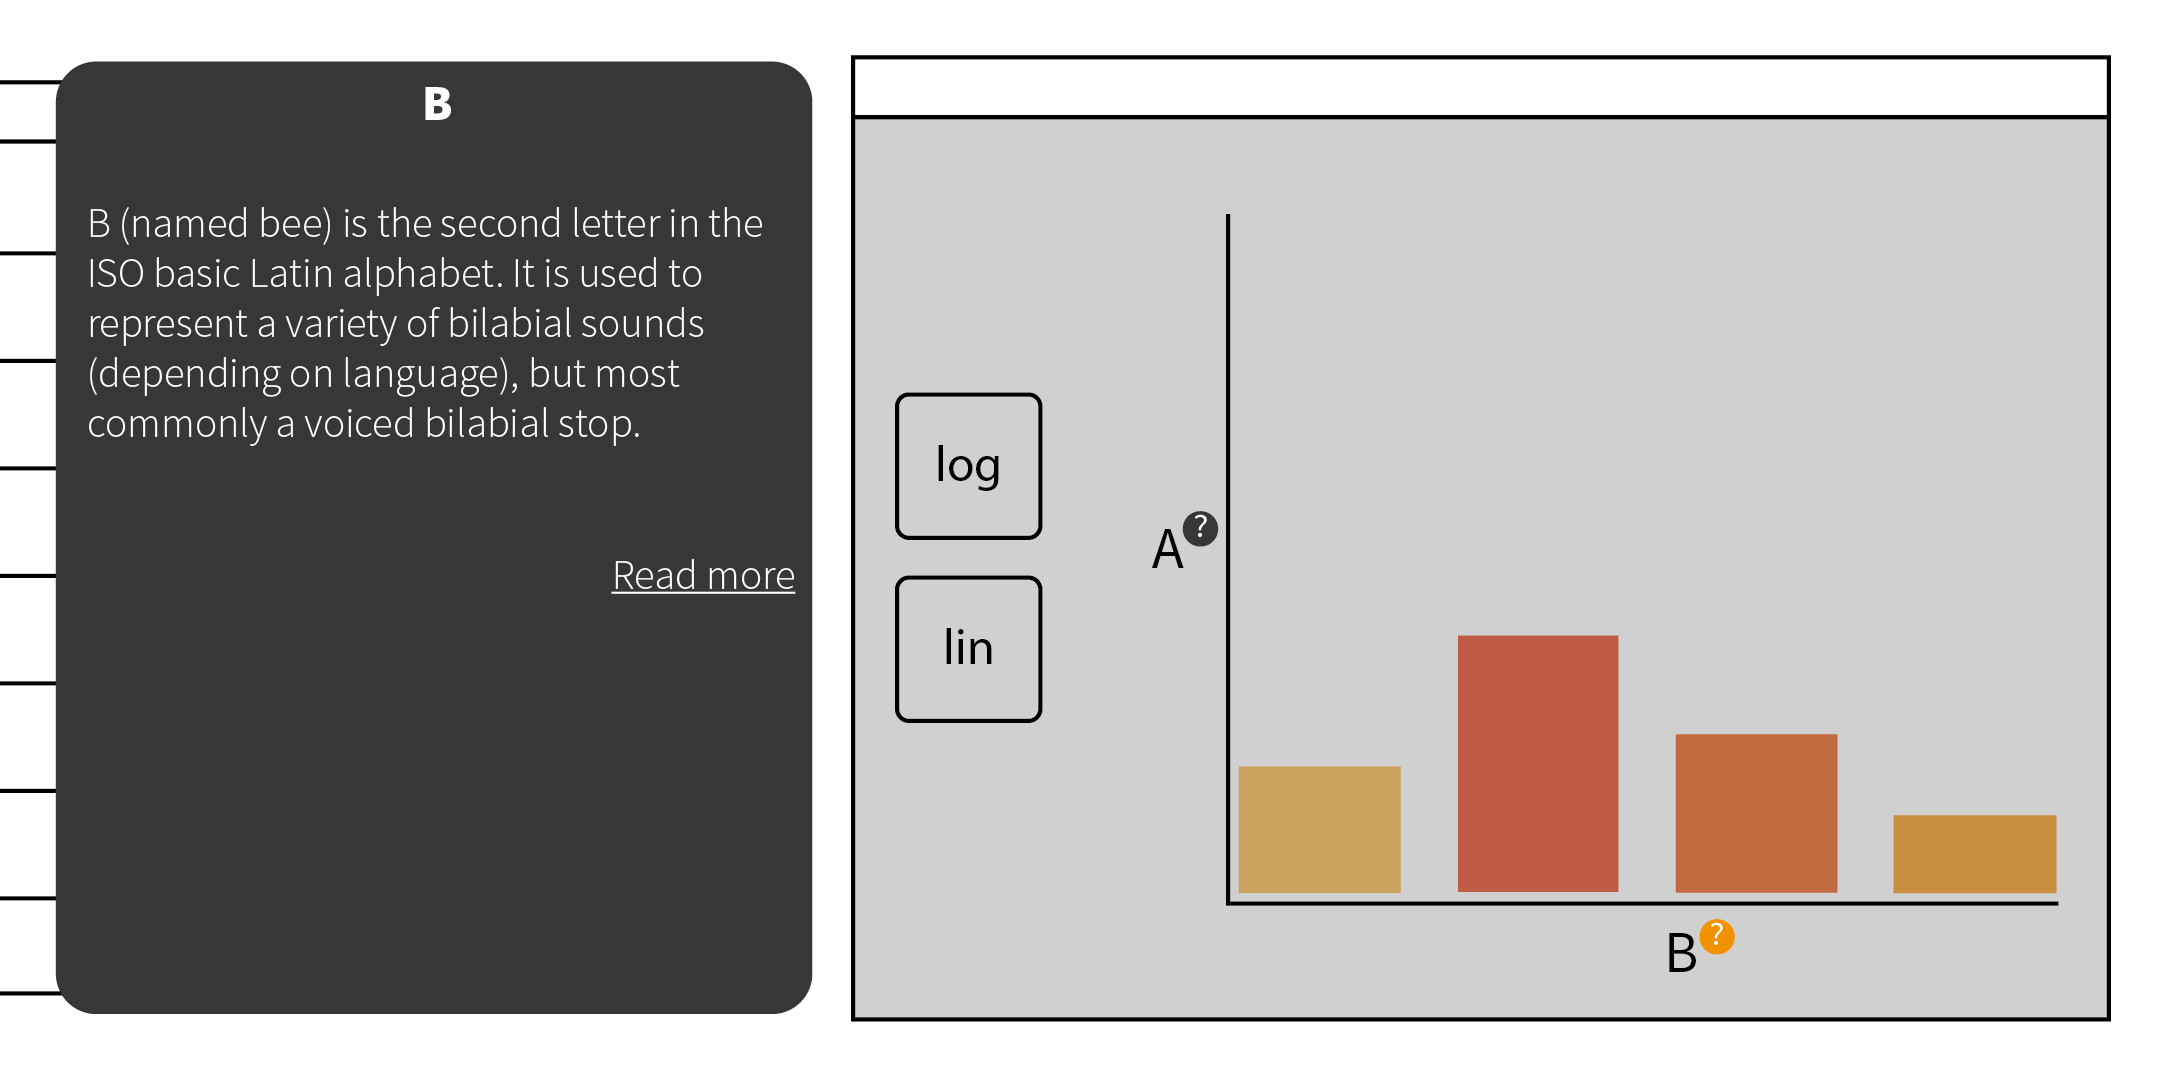
\includegraphics[width=0.5\textwidth]{images/konzeption-verlinkung.png}
   \caption{UI Mockup: Verlinkung}
   \label{figure:verlinkung}
\end{figure}

\section{Kommunikation}
\label{section:konzeption:kommunikation}

Im kompositen Infomationsvisualisierungssystem VizBoard kommunizieren Komponenten miteinander, indem sie Nachrichten austauschen (Abschnitt~\ref{section:standderforschung:grundlagen:cruise_vizboard:kommunikationsmodell}). Dieser Vorgang ist für den Benutzer nicht sichtbar und kann für Verwirrung sorgen, wenn andere Komponenten auf Interaktionen reagieren, die dort nicht getätigt wurden. Dem wird beigekommen, indem 

\begin{enumerate}
	\item die Kommunikation zwischen Komponenten sichtbar gemacht wird und
	\item die Abhängigkeiten zwischen Komponenten wie bei der Bedienung (Abschnitt~\ref{section:konzeption:bedienung}) mit Comics erklärt werden.
\end{enumerate}

\subsection{User Interface und Interaktion}
\label{section:konzeption:kommunikation:ui}

Wie im vorigen Abschnitt erläutert, wird zuerst der Nachrichtenaustausch zwischen Komponenten sichtbar gemacht (Abbildung~\ref{figure:kommunikation-step1}). Dazu wird ein Pfeil vom Sender der Nachricht zum Empfänger animiert und gezeichnet, der in der Mitte einen Brief enthält. Sollten mehrere Empfänger vorhanden sein, existiert für jeden davon ein Brief. Der Pfeil wird nicht mehr gerendert, sobald der Benutzer die Hilfe zu der Kombination (Sender, Empfänger) aufgerufen hat und verschwindet, wenn ein anderer Pfeil gerendert werden muss. Ansonsten sind zu viele Pfeile gleichzeitig im Viewport sichtbar.

\begin{figure}[htbp]
   \centering
   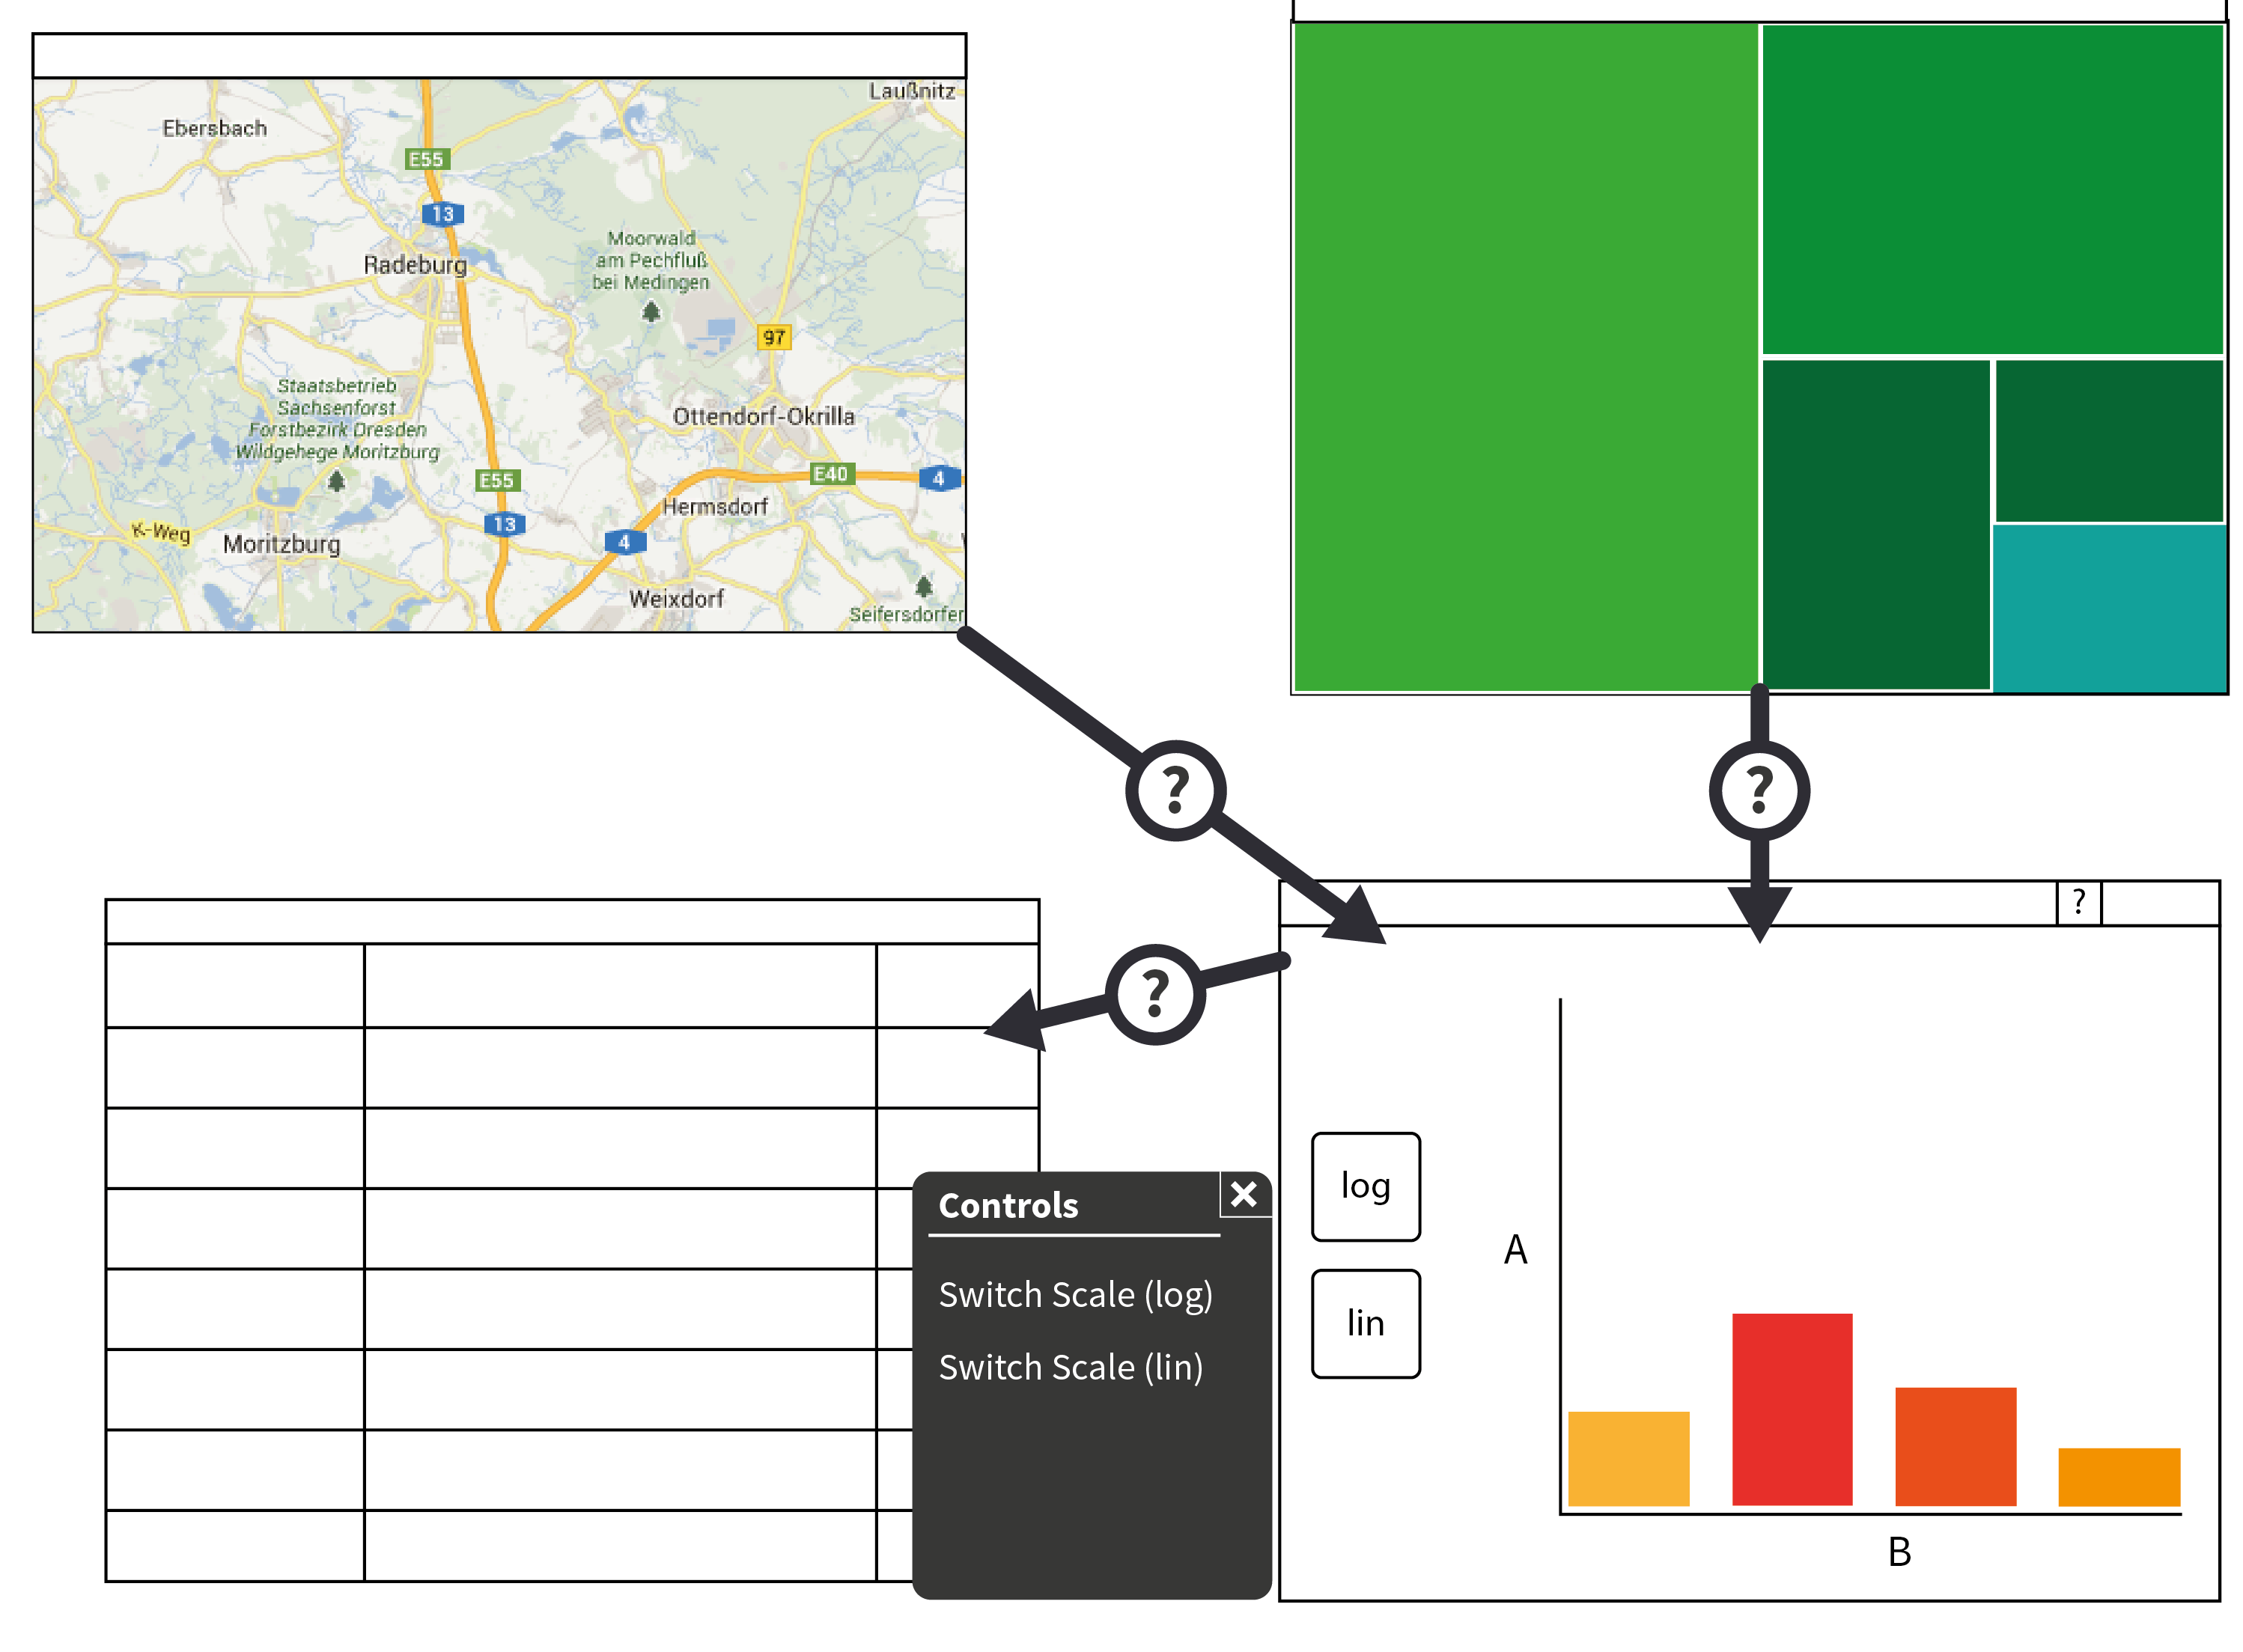
\includegraphics[width=0.5\textwidth]{images/konzeption-kommunikation-step1.png}
   \caption{UI Mockup: Kommunikation}
   \label{figure:kommunikation-step1}
\end{figure}

Die Abhängigkeiten zwischen den beiden Komponenten werden erklärt, nachdem auf den Brief geklickt wurde (Abbildung~\ref{figure:kommunikation-step2}). Ein Fenster wird geöffnet, welches einen ähnlichen Comic wie in Abschnitt~\ref{section:konzeption:bedienung} enthält. Im Unterschied dazu enthält der Comic hier fünf Panels. Im ersten wird der Empfänger der Nachricht gezeigt, da diese Komponente auf die Nachricht reagieren muss. Das zweite Panel zeigt den Sender, der den Empfänger durch die Nachricht \enquote{kontrolliert}. Die Panels drei bis fünf zeigen wie gewohnt die relevanten UI Elemente, eine notwendige Operation und das Ergebnis (den Empfänger). Wenn der Benutzer das Fenster schließt, wird auch der Pfeil unsichtbar.

\begin{figure}[htbp]
   \centering
   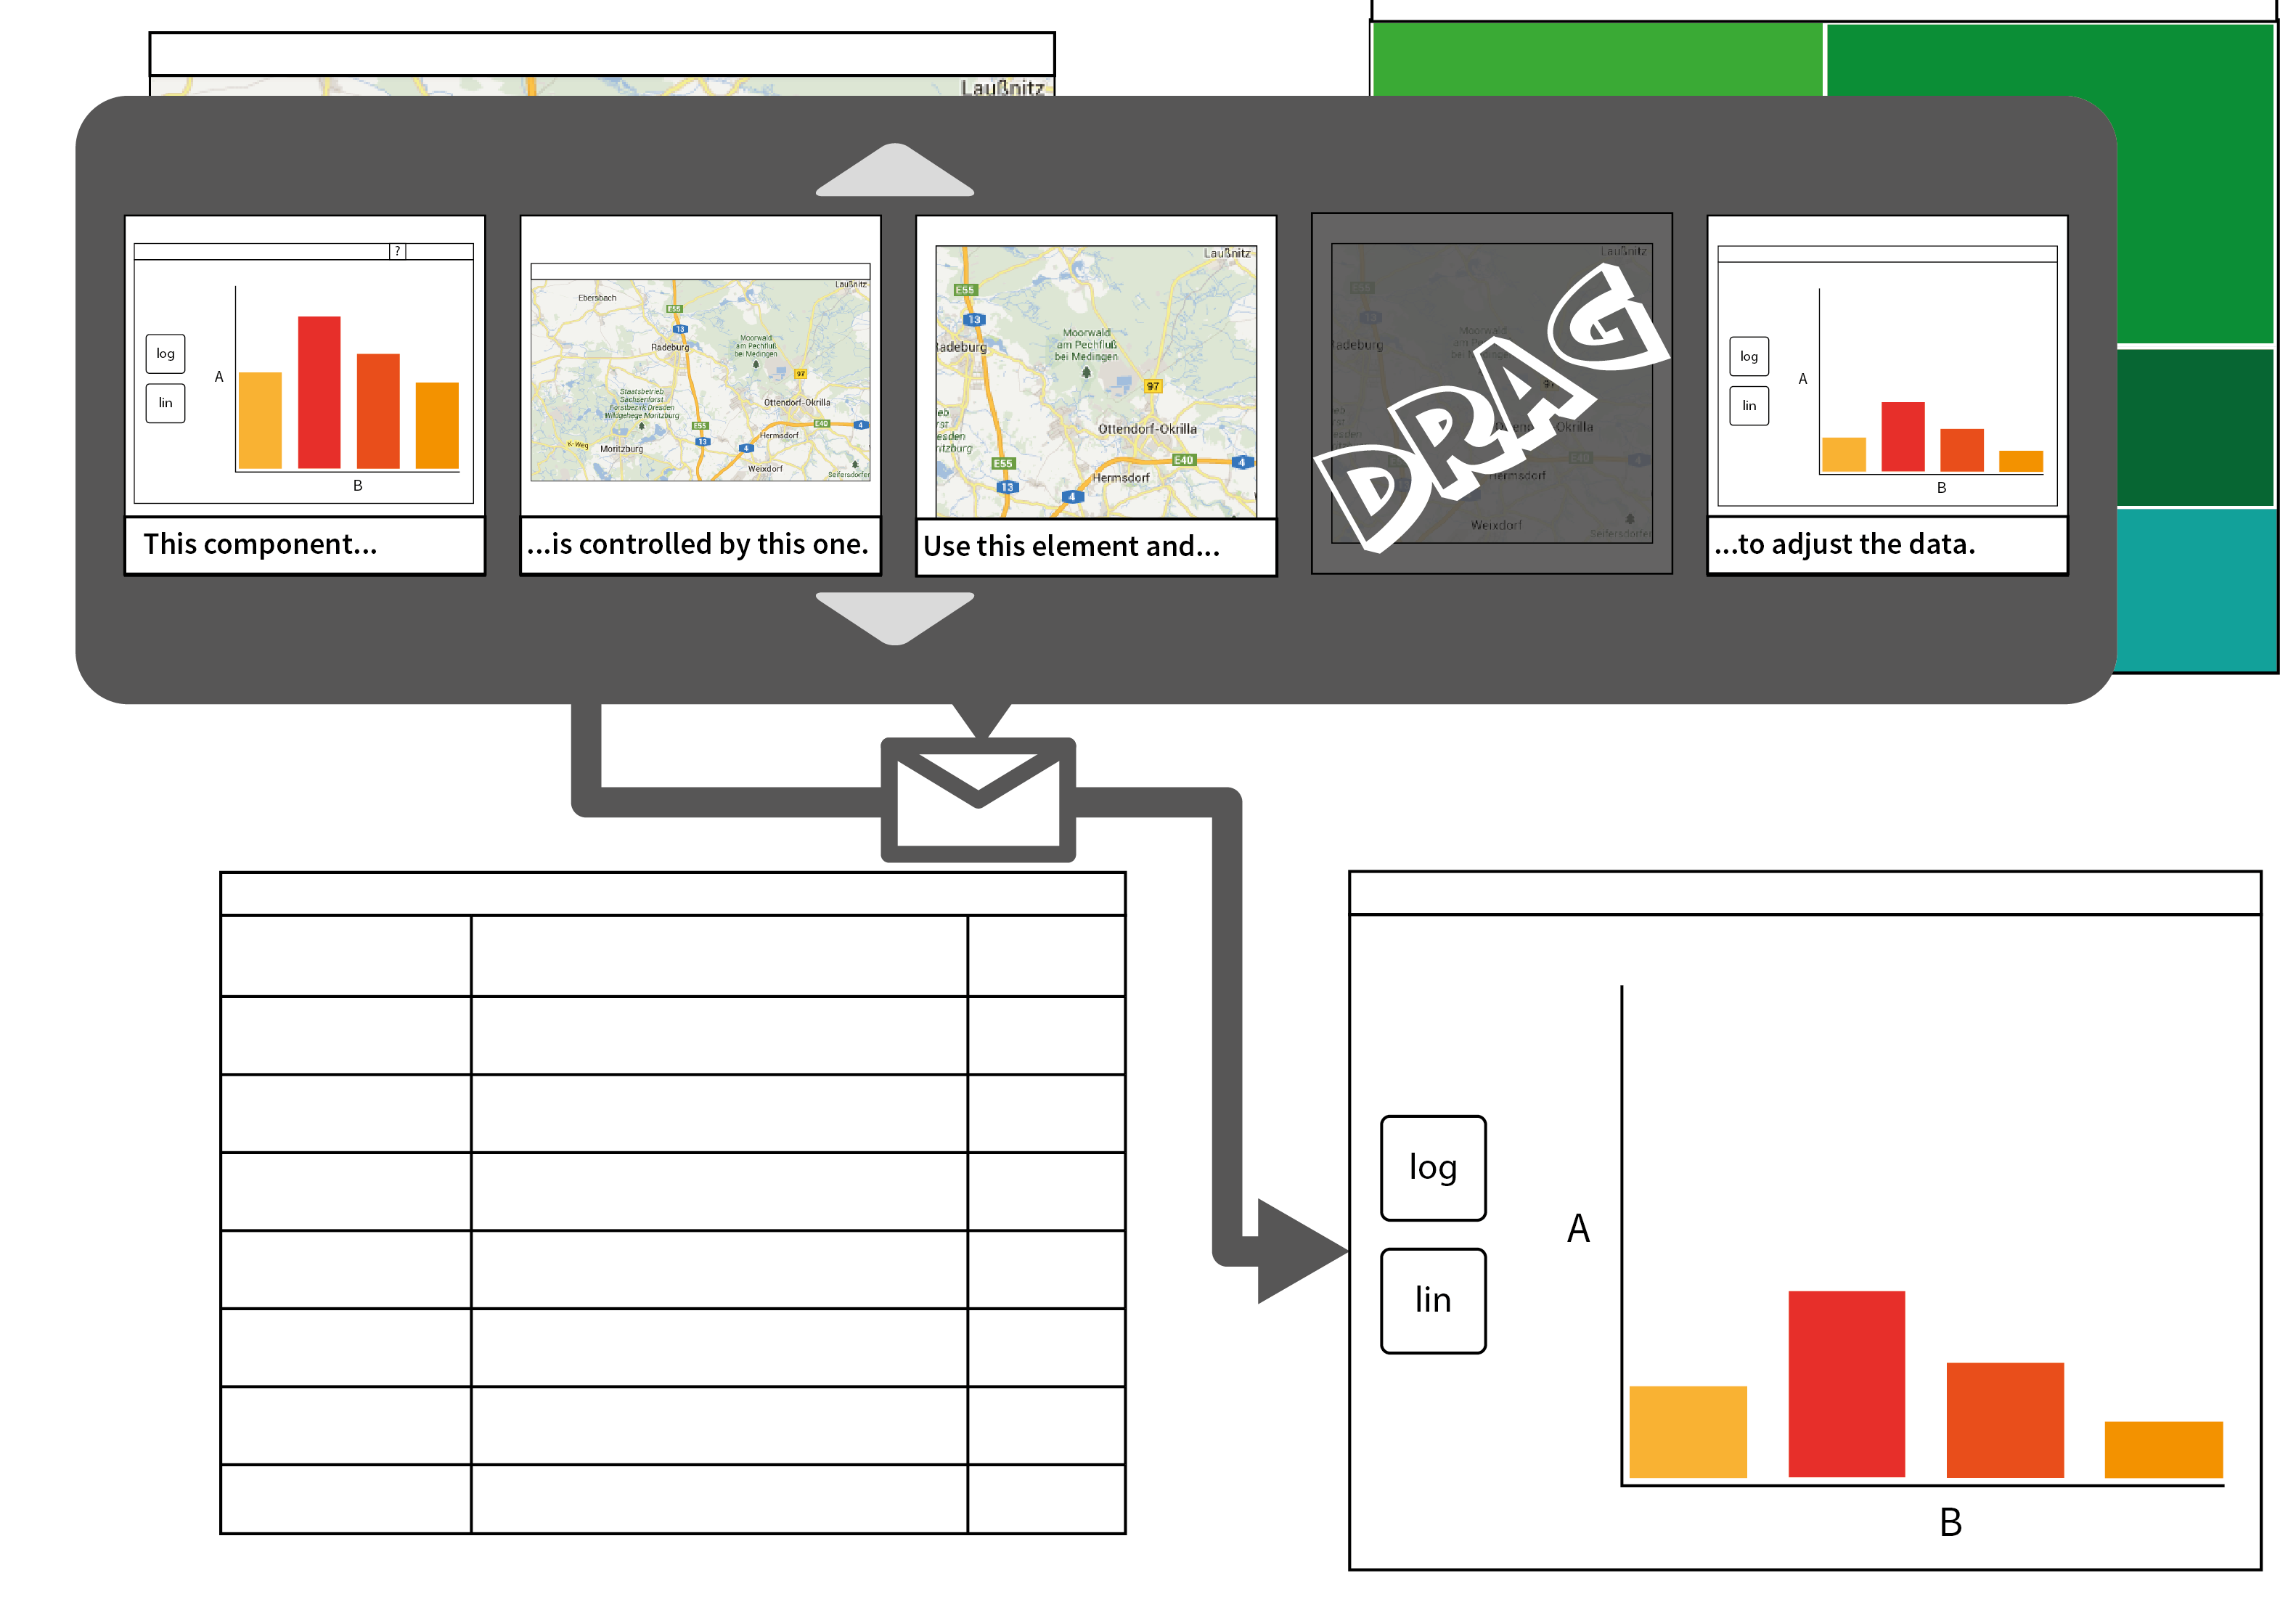
\includegraphics[width=0.5\textwidth]{images/konzeption-kommunikation-step2.png}
   \caption{UI Mockup: Comic erklärt Kommunikation. Verändern des Kartenausschnittes (Aktion: Panning, Operation: Drag) bewirkt ein Update im Balkendiagramm.}
   \label{figure:kommunikation-step2}
\end{figure}

\subsection{Backend}
\label{section:konzeption:kommunikation:backend}

Die Kommunikation zwischen Komponenten kann über den Event Broker (Abschnitt~\ref{section:standderforschung:grundlagen:cruise_vizboard}) nachvollzogen werden, da dieser zentraler Austauschpunkt für Nachrichten ist. Das Hilfesystem zeichnet Pfeile, sobald es vom Event Broker über Nachrichten informiert wird.

Für die Generierung des Comics muss das Konzept der User Assistance für Bedienung (Abschnitt~\ref{section:konzeption:bedienung:api}) nur leicht erweitert werden. Da Komponenten mit Operationen auf Nachrichten reagieren (Abschnitt~\ref{section:standderforschung:grundlagen:cruise_vizboard:kommunikationsmodell}), muss für das Ergebnis einer Operation ebenfalls ein Screenshot erstellt werden. Diese sind jetzt schon in der Komponentenbeschreibung vorhanden und können während der Panel-Generierung einfach ausgeführt werden. Sollten die Operationen Parameter erwarten, muss der Komponentenentwickler Beispieldaten in die Komponentenbeschreibung einfügen.

Zu beachten ist allerdings, dass es Operationen geben kann, welche das User Interface der Komponente nicht verändern. Das Konzept der Hilfestellung mit Comics fußt darauf, dass ein sichtbarer Unterschied zwischen den Zuständen vor und nach einer Interaktion bzw. Operation besteht. Ist jener nicht vorhanden, ergibt der Comic keinen Sinn mehr. Deswegen muss dem Komponentenentwickler eine Möglichkeit gegeben werden, Operationen zu identifizieren, für die keine Hilfe generiert werden soll.

\section{Kommentare}
\label{section:konzeption:kommentare}

% allgemeines zu kommentaren. woraus bestehen sie, was müssen sie können.

Mit Hilfe von Kommentaren können Endnutzer andere auf beobachtete Fakten der Daten wie Ausreisser oder Trends hinweisen und so zum Verständnis beitragen.
% wie können kommentare umgesetzt werden? dev vs us! warum machen wir es so wie geplant?

Prinzipiell gibt es zwei Varianten, wie Kommentare in einer InfoVis-Komponente umgesetzt werden können. In der ersten kümmert sich die Komponente darum, wie und wann sie Kommentare lädt und anzeigt. Der Vorteil daran ist, dass die Handhabung von Kommentaren speziell auf jede Komponente angepasst wird. Allerdings kann so kein einheitliches Look \& Feel gewährleistet werden. Zwar könnten Designrichtlinien Aussehen und Interaktionen vorschreiben, sie sind aber zwecklos wenn der Komponentenentwickler sie nicht einhält. Außerdem erhöht diese Variante den Entwicklungsaufwand der Komponente stark.

In der zweiten Variante ist es Aufgabe des Hilfesystems, Kommentare zu verwalten und anzuzeigen. Die vorhin genannten Nachteile werden hier zu Vorteilen: Einheitliches Look \& Feel wird sichergestellt und der Komponentenentwickler hat keinen zusätzlichen Entwicklungsaufwand. Allerdings hat das Hilfesystem auf Grund des \enquote{Black Box} Prinzips keinen Zugriff auf die in der Komponente verwendeten Daten. Aus demselben Grund kommt hinzu, dass das User Interface für Kommentare sich verschiedenen Interaktionen der Komponente wie z.\,B. scrollen, Tab wechseln, zoomen etc. anpassen muss, ohne darüber informiert zu werden. Im folgenden wird erläutert, wie diese Nachteile umgangen werden können.

\subsection{Features}
\label{section:konzeption:kommentare:features}

% ### funktionen eines kommentars

In diesem Abschnitt wird diskutiert, welche Funktionen das Kommentarsystem zur Verfügung stellen soll.

\subsubsection{URL einfügen}

Es ist wahrscheinlich, dass Benutzer zur Erklärung der Daten bzw. Visualisierung auf externe Quellen verweisen müssen. Da VizBoard ohnehin webbasiert ist, eignen sich Links in Form von URLs dafür sehr gut.

\subsubsection{Kommentar referenzieren}

Um Diskussionen und Konversationen zur Visualisierung zu fördern, müssen Kommentare einander referenzieren können \cite{Heer2007}. So wird es Benutzern erleichtert, zusammen eine Erklärung für Ausreisser oder Trends zu finden. 

\subsubsection{Voting}

Erfahrungsgemäß tragen nicht alle Kommentare gleich viel zur Diskussion bei. Man denke dabei an Hinweise auf Tippfehler oder das berüchtigte \enquote{Erster!}. Deswegen ist es notwendig, dass Benutzer Kommentare anderer bewerten können.

\subsubsection{Ranking}

Da Kommentare in einer Liste angezeigt werden und keine Buttons zum Sortieren vorgesehen sind (Abschnitt~\ref{section:konzeption:kommentare:ui}), muss das Hilfesystem die anzuzeigenden Kommentare nach einem Algorithmus sortieren. In diesen sollten sowohl die Bewertung eines Kommentars als auch die Komponente, in der er verfasst wurde und die Daten, die er referenziert, einfließen. Möglich wäre zum Beispiel nach Bewertung zu sortieren, aber Kommentare zu bestrafen, wenn sie aus anderen Komponenten stammen oder nur teilweise die gefragten Datenattribute referenzieren. Dann wird nur ein festgelegter Teil der Bewertung berücksichtigt (z.\,B. die Hälfte). So werden Kommentare aus der gleichen Komponente bevorzugt, aber solche mit hohen Bewertungen erscheinen trotzdem zuerst.

\subsubsection{Kommentar editieren}

Den eigenen Kommentar editieren zu können, ist aus verschiedenen Gründen wichtig, z.\,B. wenn der Benutzer Tippfehler ausbessern oder ein paar Absätze zur Lesbarkeit einfügen will. Wichtig ist für andere, dass dies transparent geschieht und die Diskussion nachvollziehbar bleibt. Es gibt verschiedene Lösungsmöglichkeiten:

\begin{itemize}
	\item Der Kommentar kann nicht editiert werden. So bleibt alles perfekt nachvollziehbar, aber der Benutzer kann nichts ausbessern.
	\item Der Kommentar kann nur für $x$ Minuten editiert werden, danach ist er gesperrt. Diese Variante erlaubt immerhin noch Tippfehler auszubessern, aber der Benutzer kann beispielsweise nicht nach einer Stunde eine Quelle einfügen.
	\item Der Kommentar kann beliebig editiert werden. Diese Variante ist aus Nutzersicht am Besten, aber sie muss anderen gegenüber transparent gemacht werden. Es muss sichtbar sein, dass ein Kommentar editiert wurde und wann. Im Idealfall würde auch die Originalversion eines referenzierten Kommentars mit abgespeichert, sodass diese später eingeblendet werden kann.
\end{itemize}

\subsubsection{Kommentar löschen}

Gründe, um einen Kommentar zu löschen, beinhalten unter anderem Schwachsinn (der von anderen als solcher identifiziert wurde), Beschimpfungen oder mangelnde Aktualität. Wie beim Editieren von Kommentaren ist es hier notwendig, dass der Gesprächsverlauf nachvollziehbar bleibt. Die Lösungsansätze beinhalten:

\begin{itemize}
	\item Kommentare können nicht gelöscht werden. Das könnte Benutzer davon abhalten, Kommentare zu schreiben, was auch nicht Sinn der Sache ist.
	\item Kommentare können gelöscht werden, solange keine Referenz darauf besteht. So kann ein Diskussionsverlauf konsistent bleiben, allerdings ist dieser Weg aus Nutzersicht schwer verständlich.
	\item Kommentare können beliebig gelöscht werden. Diese Variante weckt keine Ängste, den eigenen Kommentar nicht mehr löschen zu können. Es muss aber etwas mit den Referenzen auf gelöschte Kommentare geschehen, da ansonsten die Nachvollziehbarkeit der Diskussion leidet. Beispielsweise könnte die referenzierte Originalversion abgespeichert und eingeblendet werden.
\end{itemize}

\subsubsection{Bereich der Visualisierung referenzieren}

Um eine gemeinsame Grundlage für eine Diskussion zu schaffen ist es notwendig, Bereiche der Visualisierung markieren zu können, über die man in einem Kommentar spricht. Diese Bereiche können entweder Flächen, die Datenpunkte enthalten oder nicht (Bereichskommentare), oder Datenpunkte selbst sein (Punktkommentare, Abbildung~\ref{figure:datenbereiche}).

\begin{figure}[htbp]
   \centering
   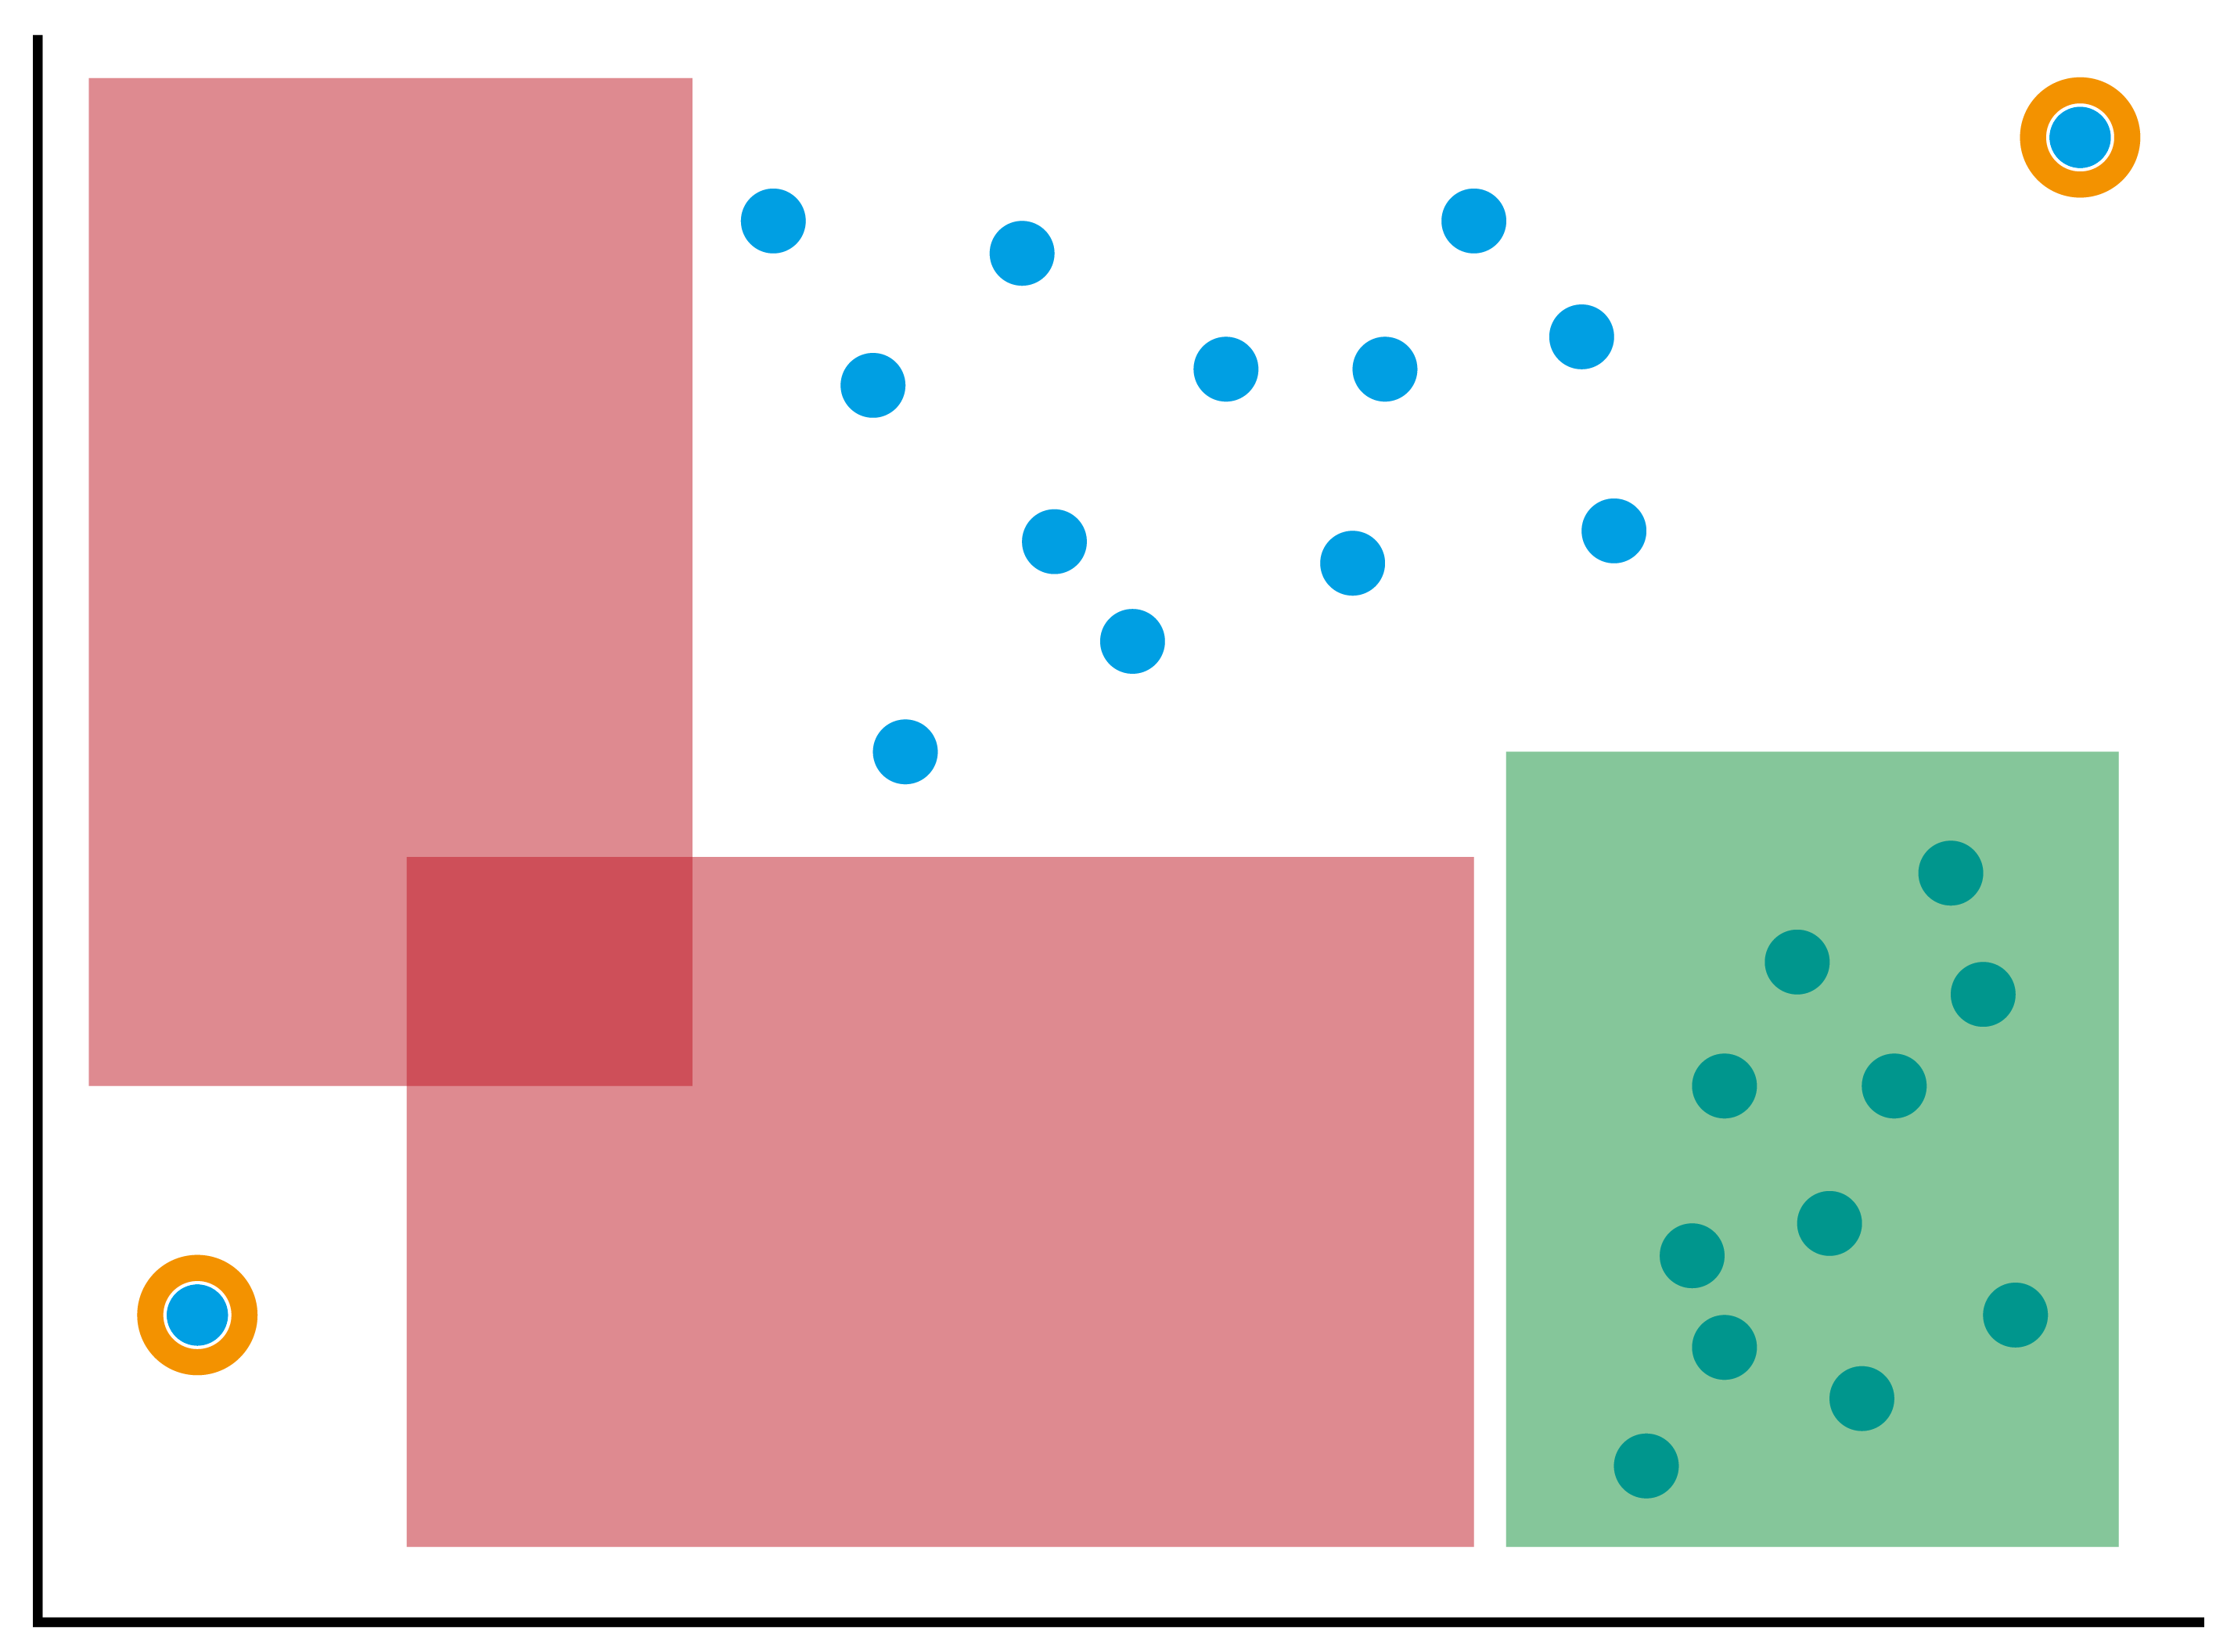
\includegraphics[width=0.5\textwidth]{images/konzeption-datenbereiche.png}
   \caption{Ein Scatterplot mit eingezeichneten Referenzierungsmöglichkeiten: Leere Bereiche (rot), nicht-leere Bereiche (grün) und einzelne Datenpunkte (orange).}
   \label{figure:datenbereiche}
\end{figure}

\subsection{API und Komponentenbeschreibung}
\label{section:konzeption:kommentare:api}

% konkreter. was gibt es für kommentare, wie unterscheiden sie sich, was ergeben sich für anforderungen daraus --> keine dynamischen daten, kein unvorhersehbares layout, keine aggregation, memento definieren, 

Wie im letzten Abschnitt beschrieben ist es notwendig, Bereiche einer Visualisierung markieren zu können.

\subsubsection{Bereichskommentare}

Um die Kommentare zu diesen Bereichen in anderen Visualisierungen wiederverwenden zu können, sollten die Daten an sich (\emph{datenbezogene Bereichskommentare}) und nicht die Fläche der Visualisierung (\emph{ortsbezogene Bereichskommentare}) referenziert werden. Damit das möglich ist, müssen drei Voraussetzungen gegeben sein:

\begin{enumerate}
	\item Die grafische Repräsentation muss Werte von Variablen auf die Position kodieren, damit eine Transformation zwischen kartesischen Koordinaten und Daten durchgeführt werden kann. Das ist beispielsweise bei einem Scatterplot der Fall, bei einer Treemap nicht. Dort sind Größe und Farbe die visuellen Attribute.  
	\item Die Komponente muss eine Operation bereitstellen, welche kartesische Koordinaten $(x_1,y_1)$ in Datenbereiche (2000 \$, 14. Mai 1998) transformiert sowie deren Umkehrung. Komponenten sind \enquote{Black Boxes} und es kann deswegen keine Annahme über die verwendete Skala (linear oder logarithmisch) oder andere Interna getroffen werden. Aus diesem Grund ist es nicht möglich, aus Auswahlkoordinaten $(x_1,y_1,x_2,y_2)$ direkt auf Daten zu schließen.
	\item Die Komponente darf keine Datenverarbeitung in Form von Aggregationen o.\,ä. durchführen, da diese Daten nicht im Data Repository gespeichert sind und es folglich keine Daten enthält, die referenziert werden könnten.
\end{enumerate}

Erfüllt eine Komponente diese Bedingungen nicht vollständig, können nur ortsbezogene Bereichskommentare eingesetzt werden. Wenn datenbezogene Bereichskommentare angezeigt und von anderen Benutzern nachvollzogen werden sollen, muss das Hilfesystem die Komponente in den damals aktiven Zustand zurücksetzen können, da ansonsten die referenzierten Bereiche andere Daten enthalten. Diese Tatsache führt zu weiteren Anforderungen an die Komponente:

\begin{enumerate}
	\setcounter{enumi}{3}
	\item Die Komponente darf keine externen Daten anzeigen, wie zum Beispiel die neuesten Tweets eines Twitter-Accounts. Diese unterliegen nicht der Kontrolle von VizBoard und können nachträglich editiert oder gelöscht werden. \todo{Elias}
	\item Das Layout der Komponente muss vollständig reproduzierbar sein, also zum Beispiel kein Force Directed Layout \cite{Fruchterman1991}.
	\item Die Komponente muss dem Hilfesystem einen Weg zur Verfügung stellen, mit dem Zustände (wie z.\,B. Zentrum und Zoomlevel einer Karte) gespeichert und vollständig wiederhergestellt werden können.
\end{enumerate}

Bezüglich der letzten Anforderung bietet sich ein Memento-Pattern \cite{Gamma1994} an:

\begin{quote}
Without violating encapsulation, capture and externalize an object's internal state allowing the object to be restored to this state later.
\end{quote} 

Dazu werden zwei Methoden \texttt{getMemento()} und \texttt{setMemento(m)} zur API der Komponente hinzugefügt, mit denen das Hilfesystem den Zustand der Komponente speichern und wiederherstellen kann. Eine andere Möglichkeit wäre das Format des Mementos -- also welche Properties es ausmachen -- in der Komponentenbeschreibung anzugeben. Das Hilfesystem könnte die Werte dieser Properties bei der Wiederherstellung des Zustands setzen. Diese Variante hat aber den Nachteil, dass PropertyLinks (Abschnitt~\ref{section:standderforschung:grundlagen:cruise_vizboard}) darauf registriert sein können. Sie könnten in anderen Komponenten unerwünschte Aktionen ausführen, während der Zustand der Komponente für Kommentare zurückgesetzt wird. Deswegen wird das Memento von den Properties getrennt.

Außerdem nötig: Den EventBroker pausieren, sodass sich die Komponente während Kommentare angezeigt werden nicht ändert. Plus: Wie resümmieren, wenn inzwischen 5 Events ankamen?

\subsubsection{Punktkommentare}

% speichern
Mit Datenpunkten verhält sich die Situation etwas einfacher als bei Bereichen. Der Komponentenentwickler kann ihre URI durch ein Datenattribut (\texttt{data-*}) an DOM Elementen, welche einen Datenpunkt repräsentieren, angeben. Dadurch kann das Hilfesystem mit CSS Selektoren herausfinden, welche DOM Elemente welche Datenpunkte darstellen und diese auswählbar machen, sollte ein Kommentar hinzugefügt werden. Wird der Kommentar abgeschickt, muss die Komponente dem Hilfesystem zuerst mitteilen, welche Werte die visualisierten Attribute eines Datenpunkts haben. Das kann nicht automatisch aus dem DOM Element berechnet werden, weil der Maßstab unbekannt ist: Entspricht eine Fläche von $100\times100$~Pixel in der Treemap 10~Quadratmetern oder 1000~Hektar? Der Maßstab kann auch nicht in der Komponentenbeschreibung angegeben werden, weil er (abhängig von der Größe der Komponente) variabel ist. Bei einer Breite von 500~Pixel wäre er z.\,B. $1:100$, bei 250~Pixel Breite aber schon $1:200$. Die URI des Datenpunkts sowie die Werte der Attribute werden im Kommentar gespeichert, sodass sie in anderen Visualisierungen wiederverwendet werden können.

% laden
Beim Laden von Punktkommentaren zählt das Hilfesystem erst die Anzahl von Kommentaren pro Datenpunkt und stellt diese Anzahl über dem visualisierten Datenpunkt dar. Das ist möglich, weil über die URI und CSS Selektoren die entsprechenden DOM Elemente identifiziert werden können.


\subsection{User Interface und Interaktion}
\label{section:konzeption:kommentare:ui}

% ### user interface & interaktion

In der Titelleiste gibt es zwei Buttons mit einem abgewandelten Sprechblasen-Icon, einmal ist ein Auge in der Sprechblase (Kommentare ansehen) und einmal ein Pluszeichen (Kommentar hinzufügen).

Wenn der Benutzer einen Kommentar verfassen will, erscheint eine Sidebar mit einer Textbox und einem Buttons zum Bestätigen (Abbildung~\ref{figure:kommentare-step4}). Abgebrochen wird nachdem der Benutzer außerhalb der Sidebar klickt. Der Benutzer kann nun ein oder mehrere, nicht überlappende Rechtecke in der Visualisierung erstellen oder Datenpunkte markieren (linker Balken in Abbildung~\ref{figure:kommentare-step4}). Das Hilfesystem setzt die Komponente in den Ausgangszustand zurück, sobald der Benutzer bestätigt oder abgebrochen hat.

\begin{figure}[htbp]
   \centering
   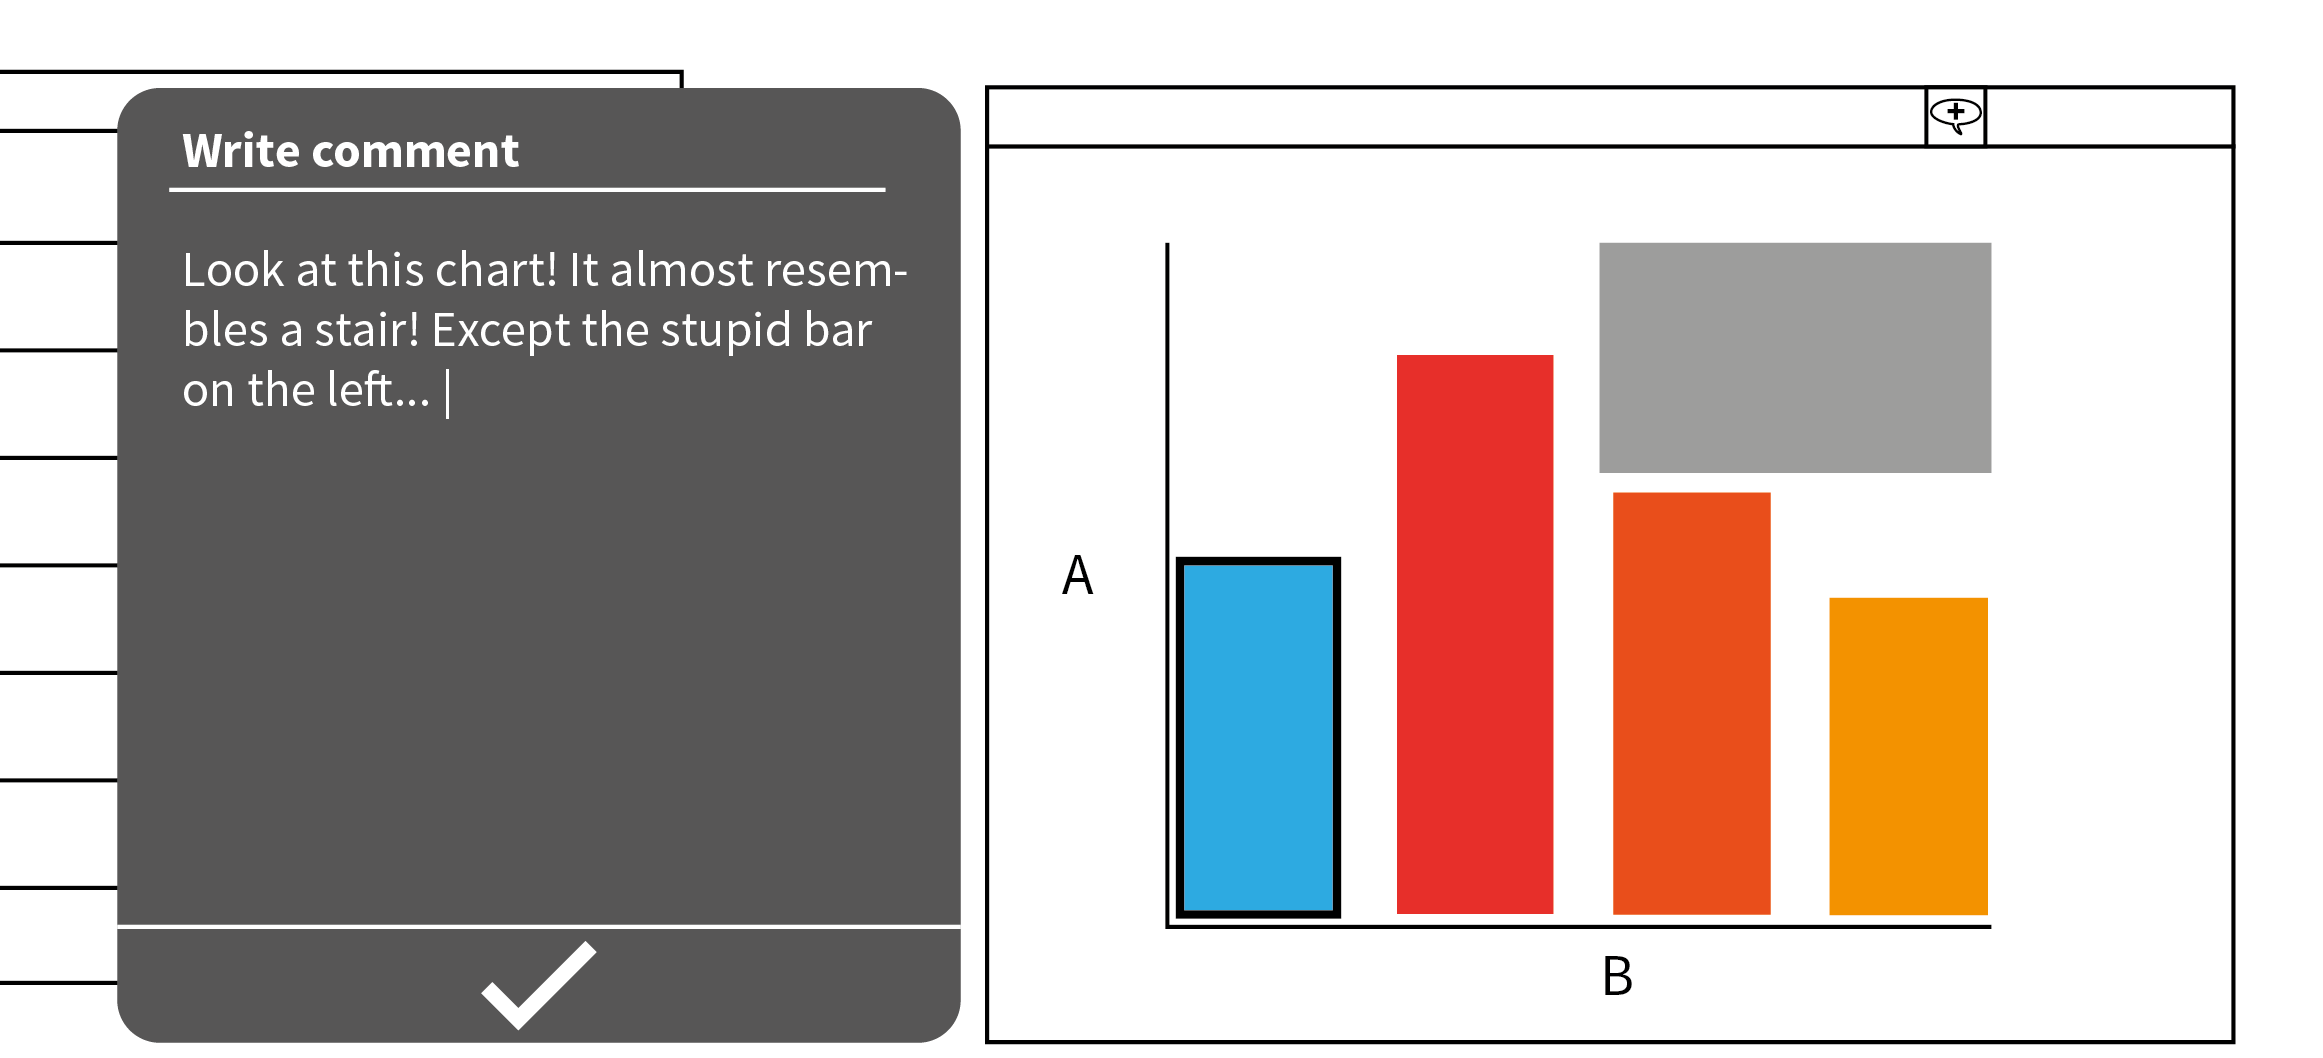
\includegraphics[width=0.5\textwidth]{images/konzeption-kommentare-step4.png}
   \caption{UI Mockup: Kommentar hinzufügen}
   \label{figure:kommentare-step4}
\end{figure}

Möchte der Benutzer Kommentare anderer lesen, wechselt der Inhalt der Sidebar zu einer Liste aller in dieser Komponente bzw. zu diesen Daten verfassten Kommentare (Abbildung~\ref{figure:kommentare-step2}). Ein Kommentar zeigt folgende Elemente.

\begin{itemize}
	\item Linke Spalte
	\begin{itemize}
		\item ID des Kommentars: Diese ist zur Referenzierung notwendig.
		\item Avatar des Benutzers und Benutzername sollen das Vertrauen der Benutzer untereinander erhöhen und so die Qualität der Kommentare verbessern \cite{Chiu2006}.
		\item Datum der Erstellung oder letzten Editierung, was jünger ist. Wurde editiert, ist das Datum kursiv geschrieben.
		\item Editieren/Löschen-Buttons, falls der Kommentar selbst verfasst wurde.
	\end{itemize}
	\item Mittlere Spalte
	\begin{itemize}
		\item Kommentartext mit Referenzen (durch \texttt{\#hash} gekennzeichnet) und URLs (unterstrichen).
	\end{itemize}
	\item Rechte Spalte
	\begin{itemize}
		\item Voting: Ein Benutzer kann einen fremden Kommentar genau einmal bewerten. Die Anzahl der Stimmen wird ebenfalls angezeigt.
		\item Antworten: Eine zweite Möglichkeit als die ID des Kommentars einzutippen. Die UI wechselt zu \enquote{Kommentar verfassen} und inkludiert die ID des betreffenden Kommentars.
		\item Bereiche anzeigen: Zeigt die vom Kommentar referenzierten Bereiche in der Visualisierung.
	\end{itemize}
\end{itemize}

Die Datenpunkte in der Visualisierung werden mit einer Anzeige, wie viele Kommentare dazu vorhanden sind, erweitert (Abbildung~\ref{figure:kommentare-step2}).

\begin{figure}[htbp]
   \centering
   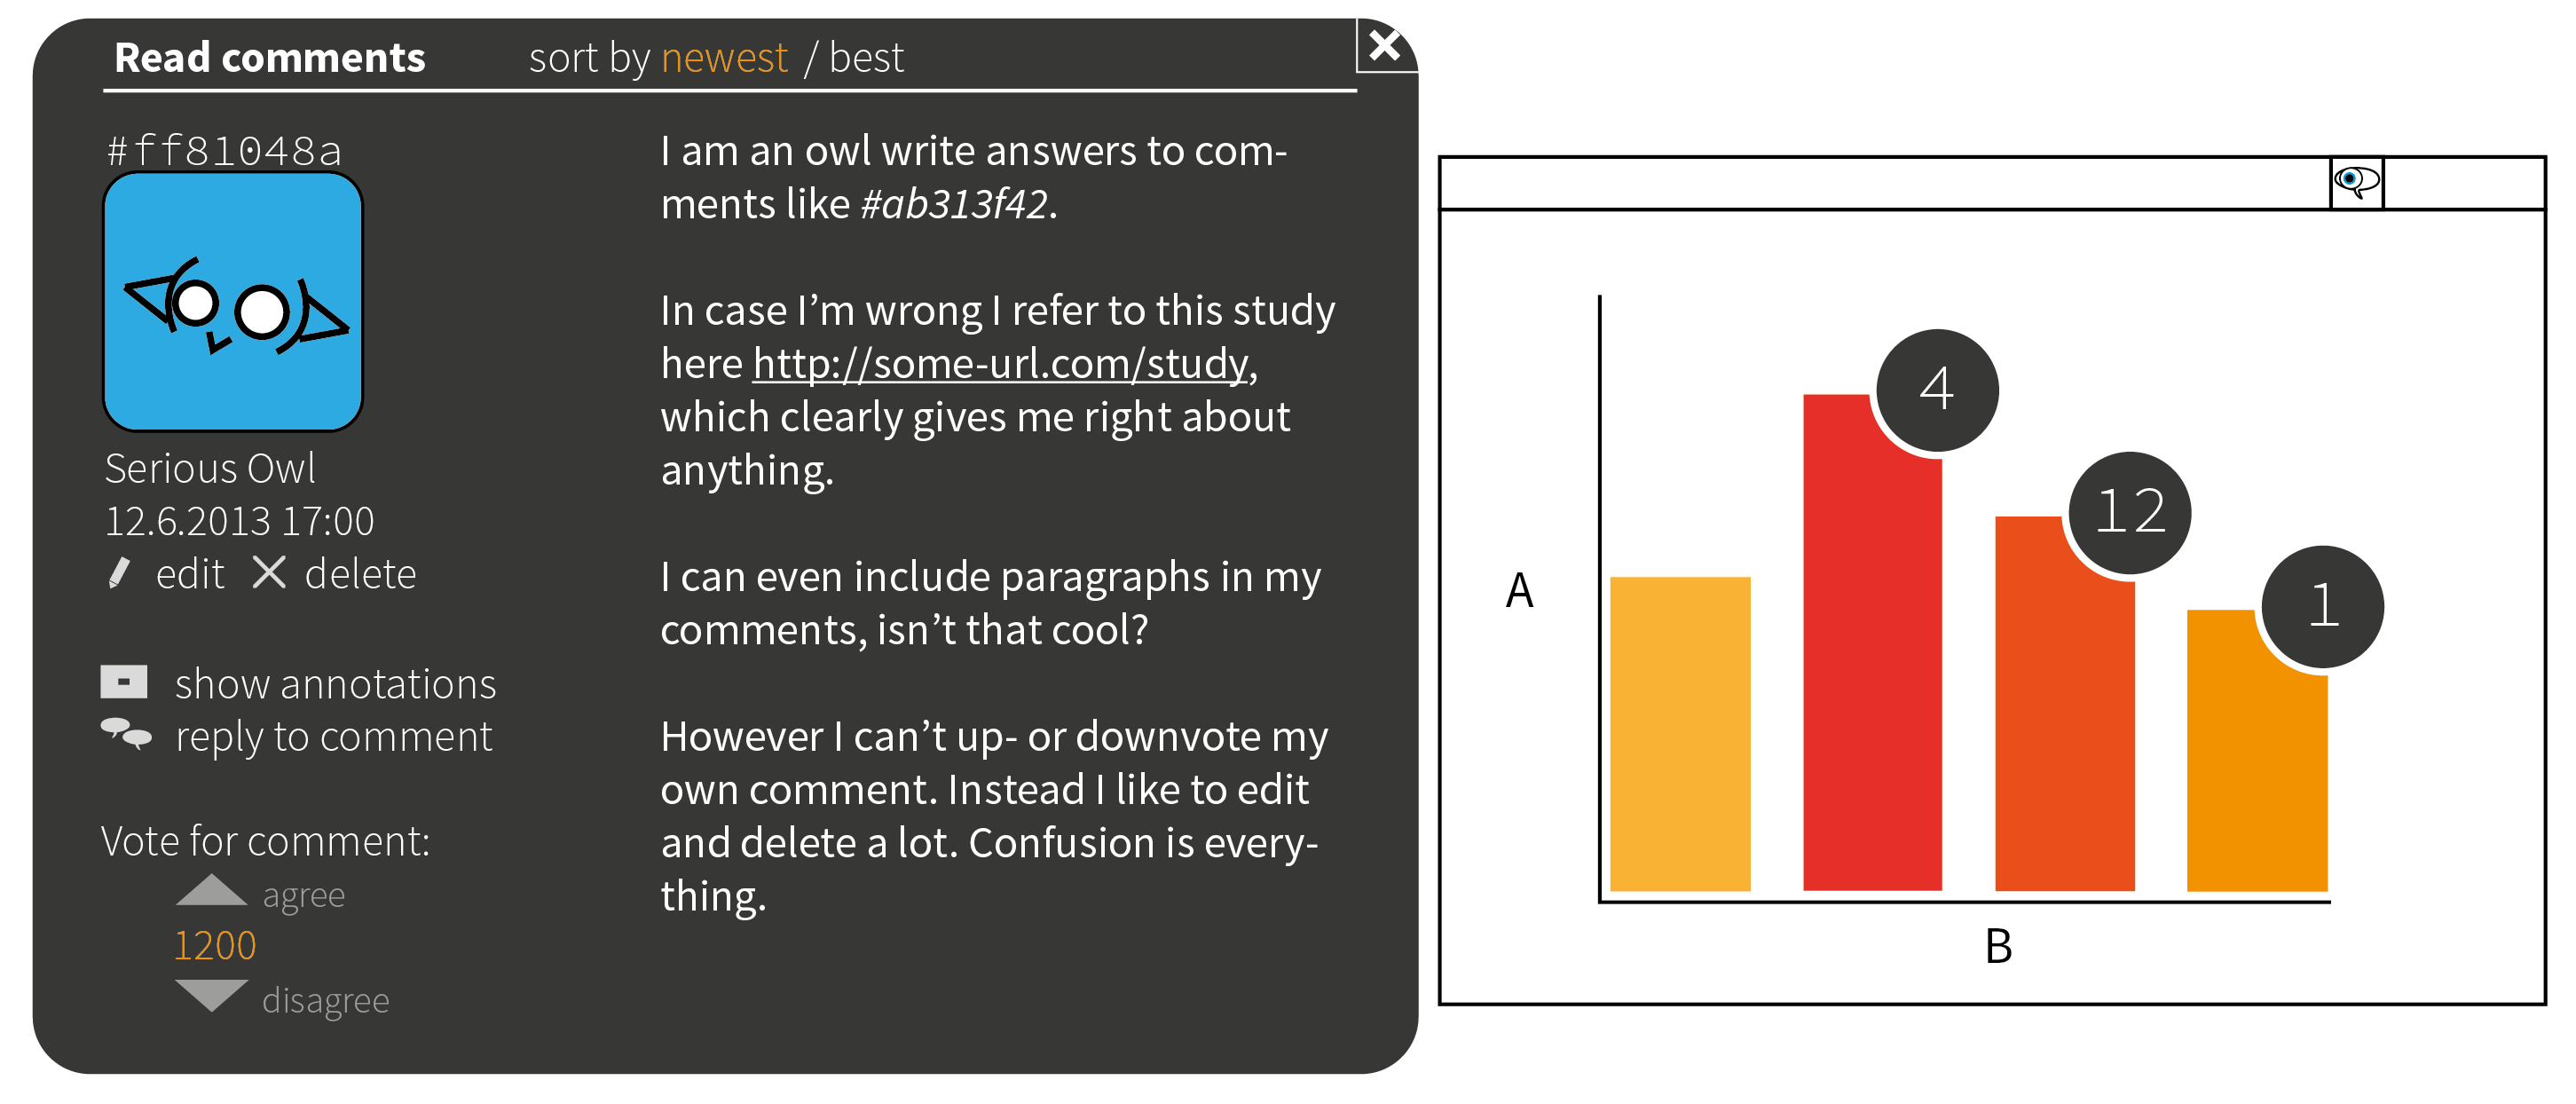
\includegraphics[width=0.5\textwidth]{images/konzeption-kommentare-step2.png}
   \caption{UI Mockup: Anzeige aller Kommentare}
   \label{figure:kommentare-step2}
\end{figure}

Diese Icons, welche die Anzahl an Kommentaren repräsentieren, können angeklickt werden. Die Sidebar enthält dann alle Kommentare, die den gewählten Datenpunkt referenzieren (Abbildung~\ref{figure:kommentare-step3c}).

\begin{figure}[htbp]
   \centering
   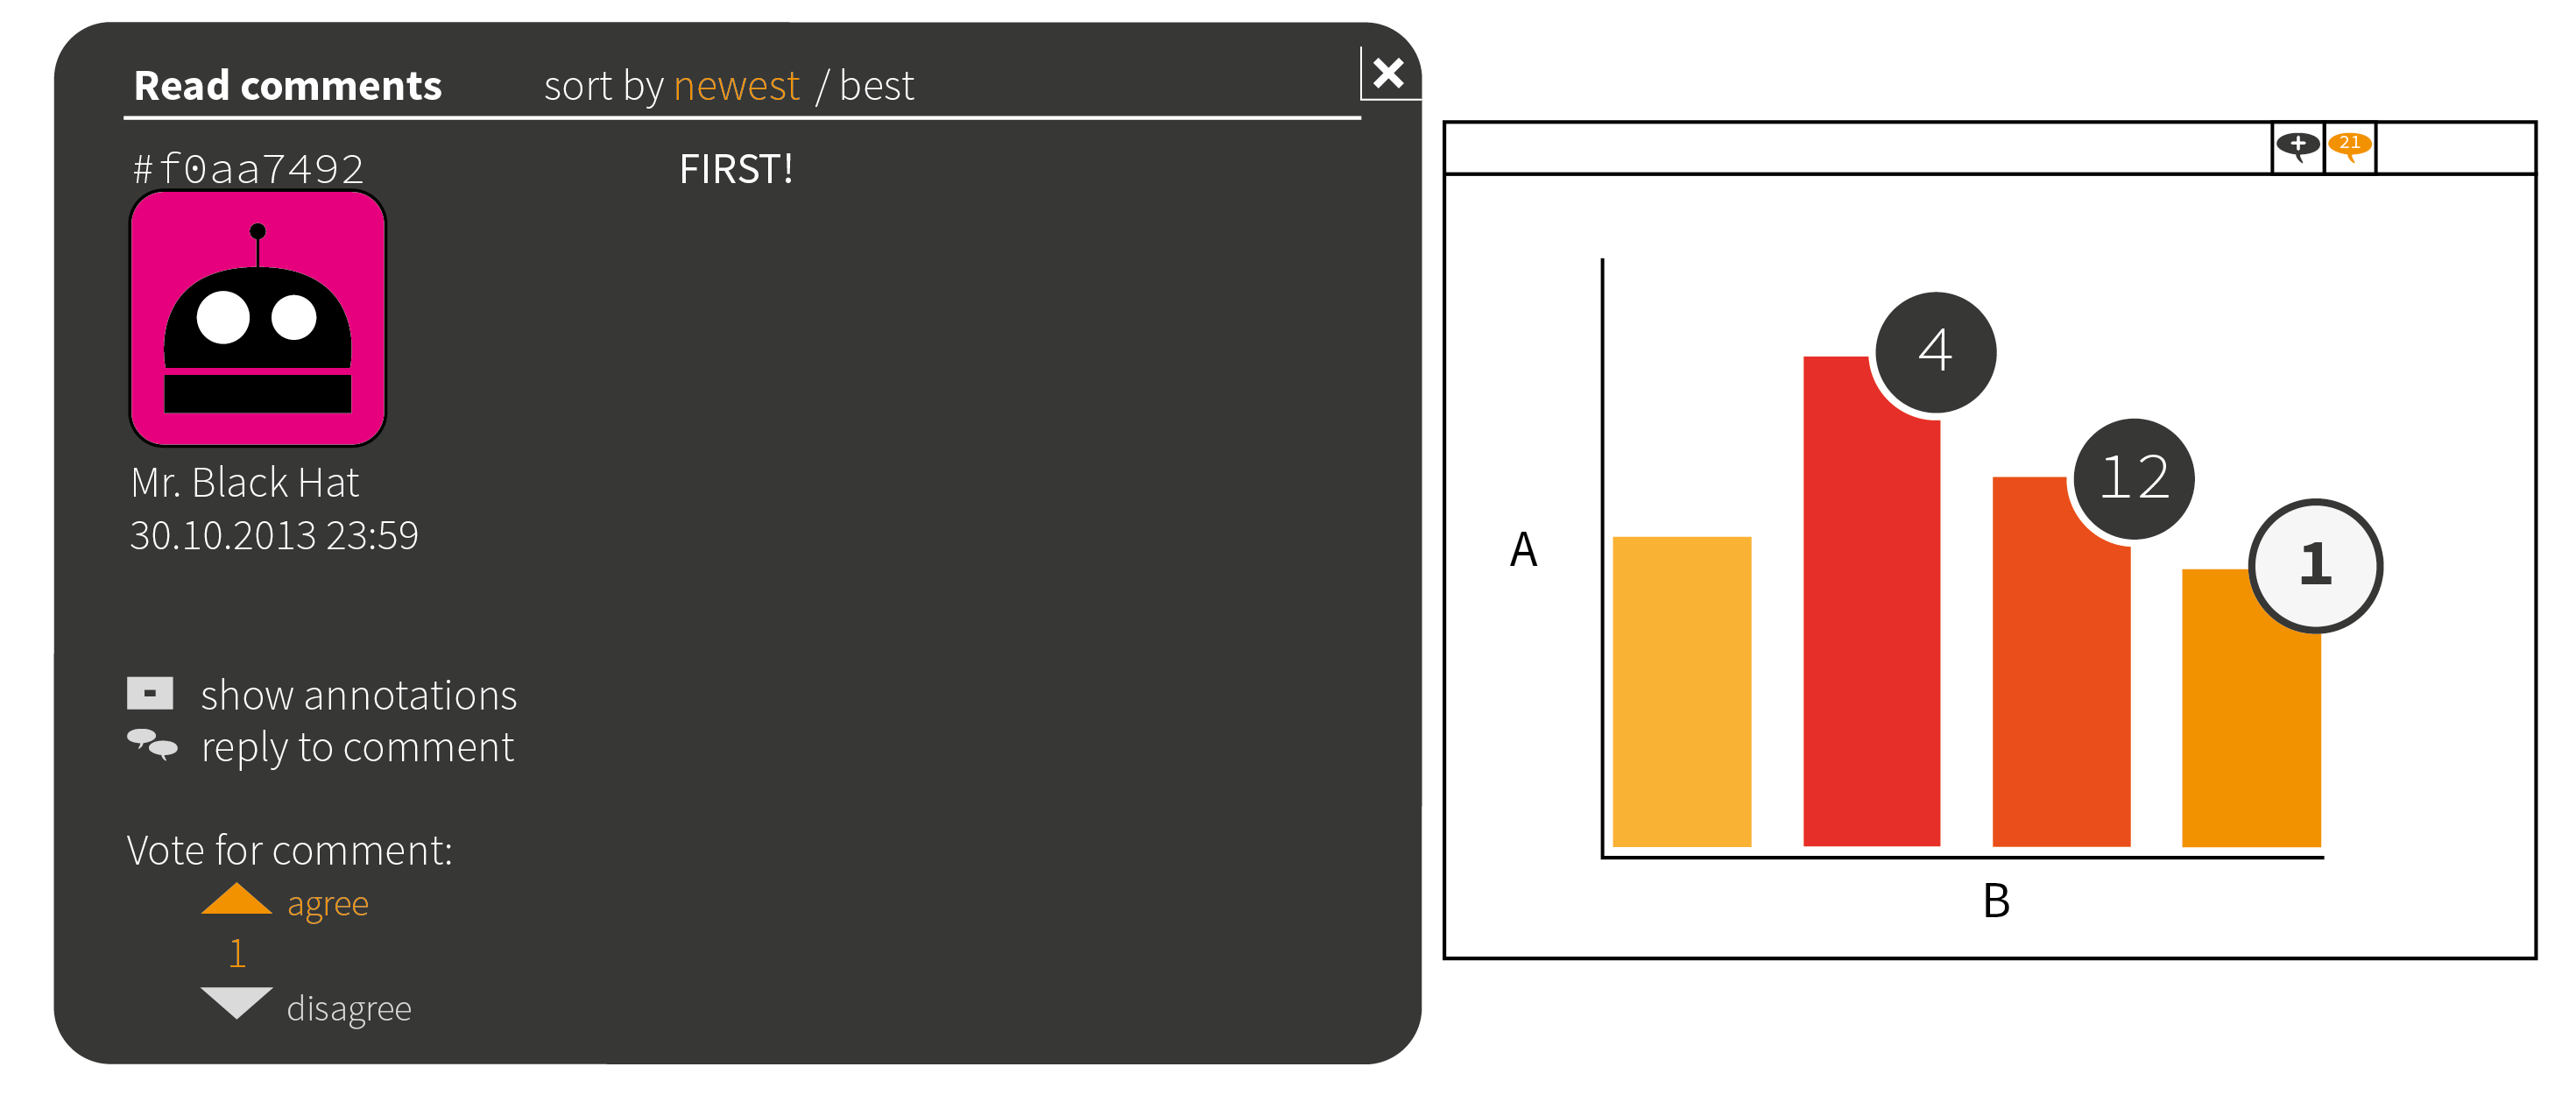
\includegraphics[width=0.5\textwidth]{images/konzeption-kommentare-step3c.png}
   \caption{UI Mockup: Alle Kommentare zum ausgewählten Datenpunkt}
   \label{figure:kommentare-step3c}
\end{figure}

Von Kommentaren referenzierte Bereiche müssen durch einen Klick auf den Button \enquote{Show} angezeigt werden. Der Viewport der Visualisierung wird dann abgedunkelt und nur die vom ausgewählten Kommentar referenzierten Bereiche bzw. Datenpunkte bleiben sichtbar (Abbildung~\ref{figure:kommentare-step3a}).

\begin{figure}[htbp]
   \centering
   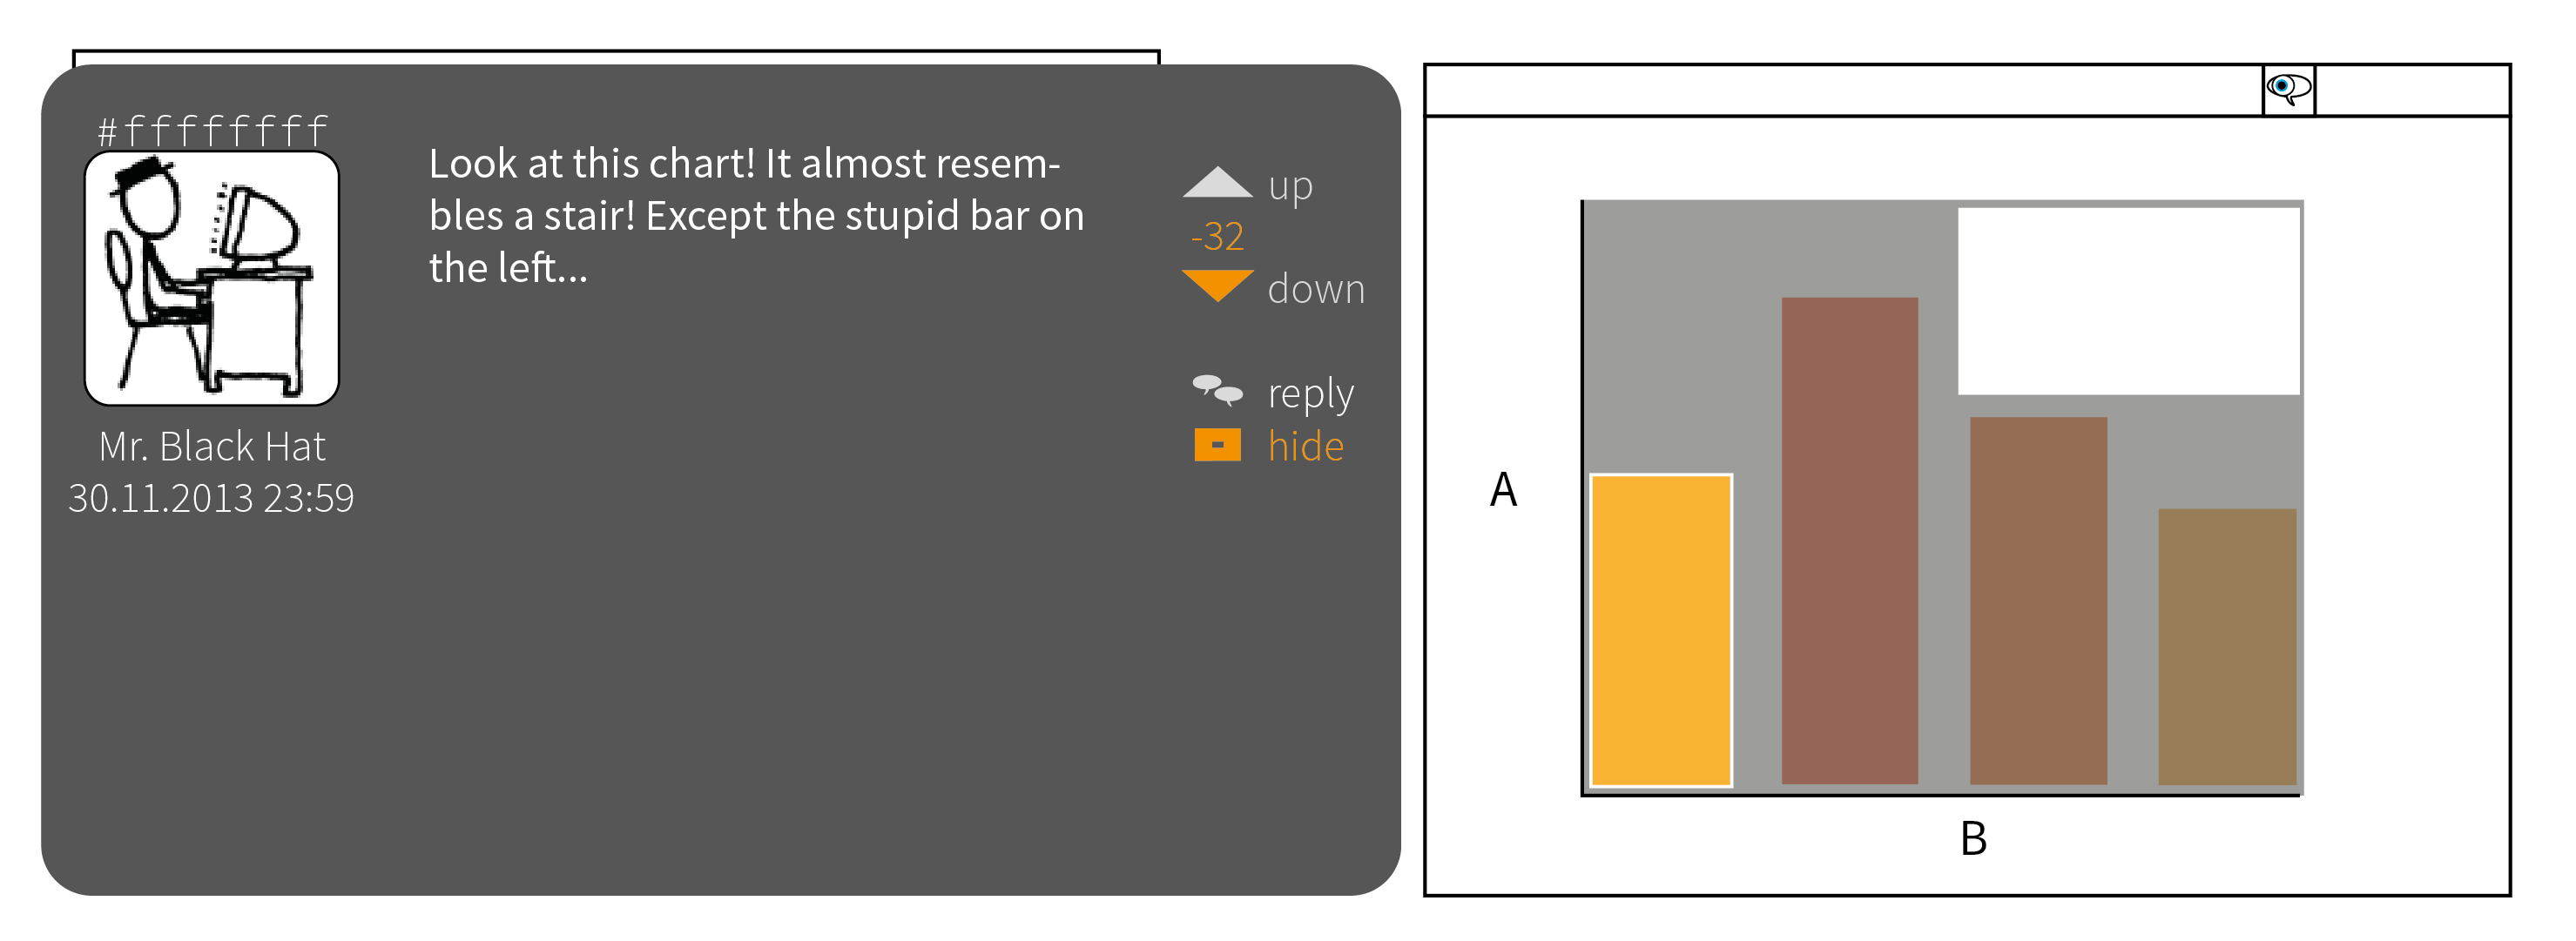
\includegraphics[width=0.5\textwidth]{images/konzeption-kommentare-step3a.png}
   \caption{UI Mockup: Ausgewählter Kommentar mit referenziertem Bereich und Datenpunkten}
   \label{figure:kommentare-step3a}
\end{figure}

\subsection{Backend}
\label{section:konzeption:kommentare:backend}

% ### backend

% welche daten enthält ein gespeichertes kommentar?

Den Ausführungen in den Abschnitten~\ref{section:konzeption:kommentare:api} und~\ref{section:konzeption:kommentare:features} nach enthält ein abgespeichertes Kommentar im DaRe folgende Daten:

\begin{itemize}
	\item ID des Kommentars, um darauf verweisen zu können.
	\item \textit{Für jede Version des Kommentars}
	\begin{itemize}
		\item Versionsnummer
		\item Zeitpunkt
		\item Kommentartext
	\end{itemize}
	\item ID der Komponente, in der der Kommentar verfasst wurde. Das ist notwendig um ortsbezogene Kommentare wiederherstellen zu können. Bei datenbezogenen Kommentaren kann eventuell ein Verweis auf die ursprüngliche Komponente erstellt werden.
	\item ID des Datensatzes, der visualisiert wurde
	\item Verfasser des Kommentars
	\item URIs der Datenattribute, die visualisiert wurden
	\item Memento der Komponente zum Zeitpunkt des Kommentars
	\item \textit{Für jeden Bereich, wenn ortsbezogen}
		\begin{itemize}
			\item Koordinaten der Auswahlrechtecke, relativ zur linken oberen Ecke der Visualisierung
			\item Größe der Visualisierung zum Zeitpunkt des Kommentars, um die Auswahlrechtecke entsprechend skalieren zu können, falls notwendig.
		\end{itemize}
	\item \textit{Für jeden Bereich, wenn datenbezogen}
		\begin{itemize}
			\item Grenzwerte der visualisierten Datenattribute
		\end{itemize}
	\item \textit{Für jeden Datenpunkt}
		\begin{itemize}
			\item URI
			\item Werte der visualisierten Datenattribute
		\end{itemize}
\end{itemize}

% wie läuft das mit speichern?

Hat ein Benutzer Bereiche und Datenpunkte referenziert, sowie einen Kommentar geschrieben, sammelt das Hilfesystem die eben beschriebenen Daten der Komponente und sendet sie ans Data Repository. Das Speichern und Laden von Kommentaren liegt in dessen Verantwortung.

% wie läuft das mit laden, vor allem wenn kommentare in anderer komponente gemacht wurden?

Sollen Kommentare angezeigt werden, schickt das Hilfesystem eine entsprechende Anfrage ans DaRe und empfängt die Daten aller relevanten Kommentare. Für ortsbezogene Bereichskommentare ist nichts weiter zu tun, sie können direkt in dieser Komponente gerendert werden. Um datenbezogene Bereichskommentare anzuzeigen, muss das Hilfesystem zuerst die Datengrenzen in Koordinaten in der Visualisierung transformieren lassen. Bei Punktkommentaren ist dies nicht nötig, weil das Hilfesystem über CSS Selektoren herausfinden kann, wo sie sich befinden sollen.

\subsubsection{Weitere Nutzung}

% wie können kommentare noch genutzt werden?

Kommentare können auch Metainformationen über die Daten oder Komponente enthalten \cite{Chen2009}. Es wäre denkbar, mittels automatischer Textklassifikation \cite{Sebastiani2002} diese Kommentare zu identifizieren und als positiv oder negativ zu kategorisieren. Daraus ließe sich wiederum eine Bewertung für die Kombination (Datensatz, Komponente) berechnen\footnote{Am einfachsten ginge das indem bei Null gestartet wird und für jeden positiven Kommentar der Zähler um eins erhöht und jeden Negativen um eins verringert wird.}. Der errechnete Wert könnte in Zukunft beim Ranking einer Komponente für einen ausgewählten Datensatz berücksichtigt werden. Wenn der Aufwand dafür gerechtfertigt werden kann, ist es auch möglich, eine -- zuvor definierte -- Ontologie aus Kommentaren zu extrahieren \cite{Alani2003}. Diese könnte zum Beispiel das Qualitätsmanagement von Komponenten automatisieren. Denkbar wäre, dass aus Kommentaren automatisch extrahiert wird, worüber sich die Benutzer beschweren. Ab einem Schwellwert kann dann der Komponentenentwickler informiert werden.

\section{Meta-Hilfe}
\label{section:konzeption:meta-hilfe}

% warum brauchen wir meta-hilfe?

In diesem Konzept wurden bisher sechs unterschiedliche Hilfefunktionen erarbeitet: Intro, Bedienung, Reporting, Verlinkung, Kommunikation und Kommentare. Diese sind zwar optisch und vom Interaktionsdesign her konsistent, bringen aber trotzdem viel zusätzliche Komplexität in die Anwendung. Um die Hilfefunktionen in vollem Umfang nutzen zu können, benötigt der Benutzer einige Informationen. Dazu gehört sowohl das Wissen, welche Hilfefunktionen existieren und wie sie aufgerufen werden, als auch konzeptionelle Dinge, wie z.\,B. dass Kommentare mit Bereichen und/oder Datenpunkten in der Visualisierung assoziiert sind. Es ist anzunehmen, dass diese Meta-Hilfe vor allem bei der ersten Nutzung von VizBoard benötigt wird. Aus diesem Grund sollte sie so unaufdringlich wie möglich gestaltet sein.

% erste lösung: statischer button

Es gibt nun verschiedene Lösungen für die Umsetzung der Meta-Hilfe. Die einfachste davon wäre ein Button in der rechten oberen Ecke, der bei Bedarf eine klassische Hilfefunktion aufruft, welche die verschiedenen Funktionen in Wort und Bild erklärt und ein Tutorialvideo enthält. Das größte konzeptionelle Problem dabei ist die dreifache Hilfception: Für VizBoard existiert ein Hilfesystem (einfach), welches wiederum erklärt werden muss (zweifach) und wo diese Erklärung zu finden ist, muss dem Benutzer ebenfalls mitgeteilt werden (dreifach). Das bedeutet relativ viel Zeit- und Klickaufwand, bis der Nutzer bei den gewünschten Informationen ist. Aber es hat auch Vorteile: Durch den statischen Hilfeknopf ist immer klar, wo weitergeholfen wird. Außerdem kann er gegebenenfalls für andere Sachen benutzt werden, beispielsweise könnte dort konfiguriert werden, ob der Pfeil in der Kommunkationshilfe bei jeder Nachricht angezeigt werden soll.

% zweite lösung: kontextabhängige dynamische hilfe

Die Alternative zum statischen Button wäre dem Benutzer dynamisch und kontextabhängig Hilfe anzubieten, beispielsweise in Form von Notifications wie in OSX. So könnten ihm Erklärungen zu den Kommentaren angeboten werden, sobald er auf den Kommentar-Button geklickt hat oder eine allgemeine Hilfe, wenn er längere Zeit keine Aktion ausgeführt hat. Der große Vorteil daran ist, dass nur die Benutzer die Meta-Hilfe sehen, welche sie auch benötigen. Allerdings hat diese Lösung zwei Nachteile. Zunächst ist es so, dass Notifications nach einer festgelegten Zeitspanne wieder verschwinden müssen, weil sie sonst stören. Dadurch ist es dem Benutzer unmöglich, aus eigener Initiative zur Meta-Hilfe zu gelangen. Davon abgesehen müssen für die kontextabhängige Hilfe einige Probleme bewältigt werden, wenn sie wie gewünscht funktionieren soll. Das Hilfesystem muss Regeln kennen, wann Hilfe angeboten werden soll. Die Reaktionen des Benutzers darauf sollen bewertet werden und zusammen mit dem Anwendungskontext wieder in die Wissensbasis einfließen, damit das System daraus lernen und neue Regeln inferieren kann. Das würde den Rahmen dieser Arbeit sprengen und kann in zukünftigen Forschungsarbeiten behandelt werden. Dann können statische und dynamische Hilfe zusammen eingesetzt werden.

\subsection{User Interface und Interaktion}

Der Button für die Meta-Hilfe befindet sich in der rechten oberen Ecke des Viewports (Abbildung~\ref{figure:meta-step1}). Er ist rot, damit er vom Benutzer bemerkt wird und rund, weil er so aus dem bisher verwendeten optischen Konzept ausbricht und auffällt, aber nicht fehl am Platz wirkt.

\begin{figure}[htbp]
   \centering
   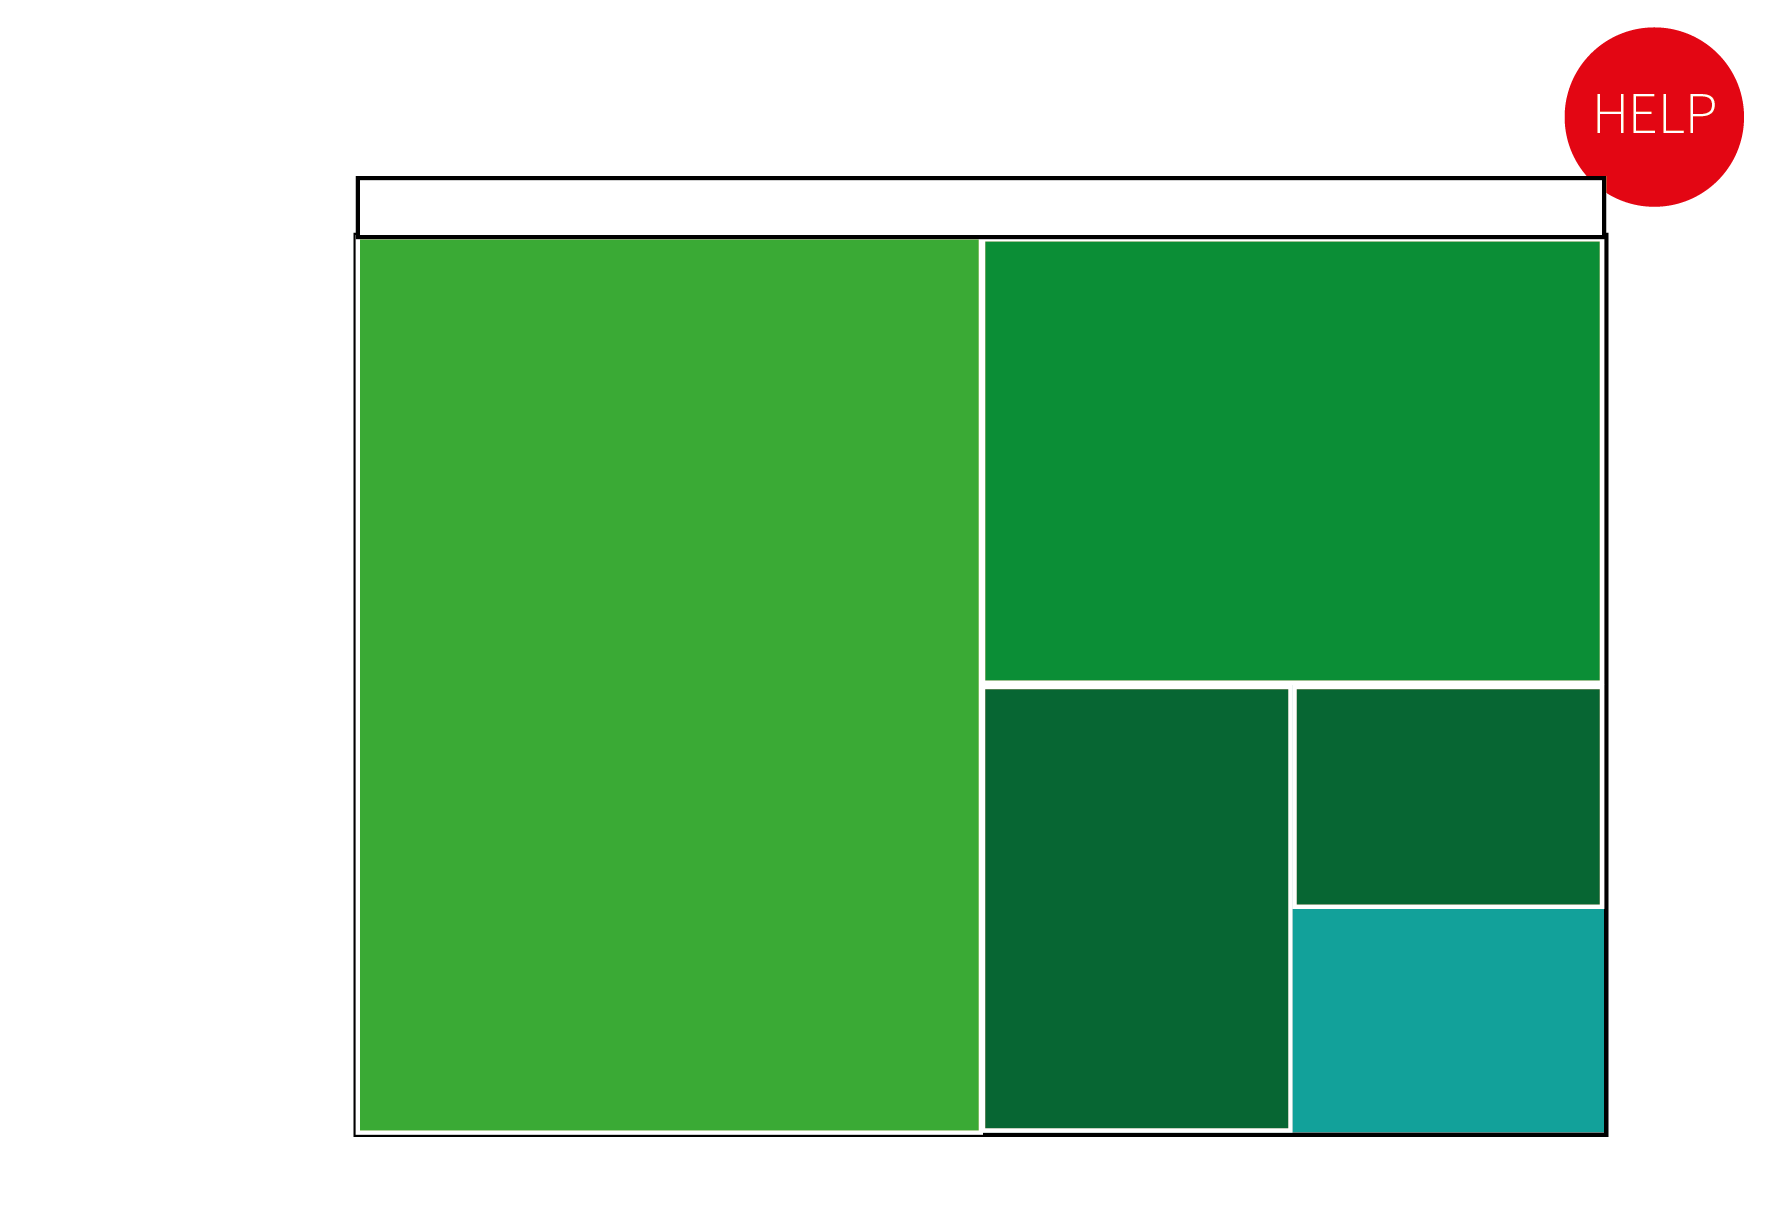
\includegraphics[width=0.5\textwidth]{images/konzeption-meta-step1.png}
   \caption{UI Mockup: Statischer Button für Meta-Hilfe}
   \label{figure:meta-step1}
\end{figure}

Nachdem der Benutzer darauf geklickt hat, wird der Viewport abgedunkelt und ein Fenster überblendet, welches Hilfe zu verschiedenen Themen enthält (Abbildung~\ref{figure:meta-step2}). Von dort können ebenfalls die verschiedenen Hilfefunktionen (wie z.\,B. das Intro) aufgerufen werden.

\begin{figure}[htbp]
   \centering
   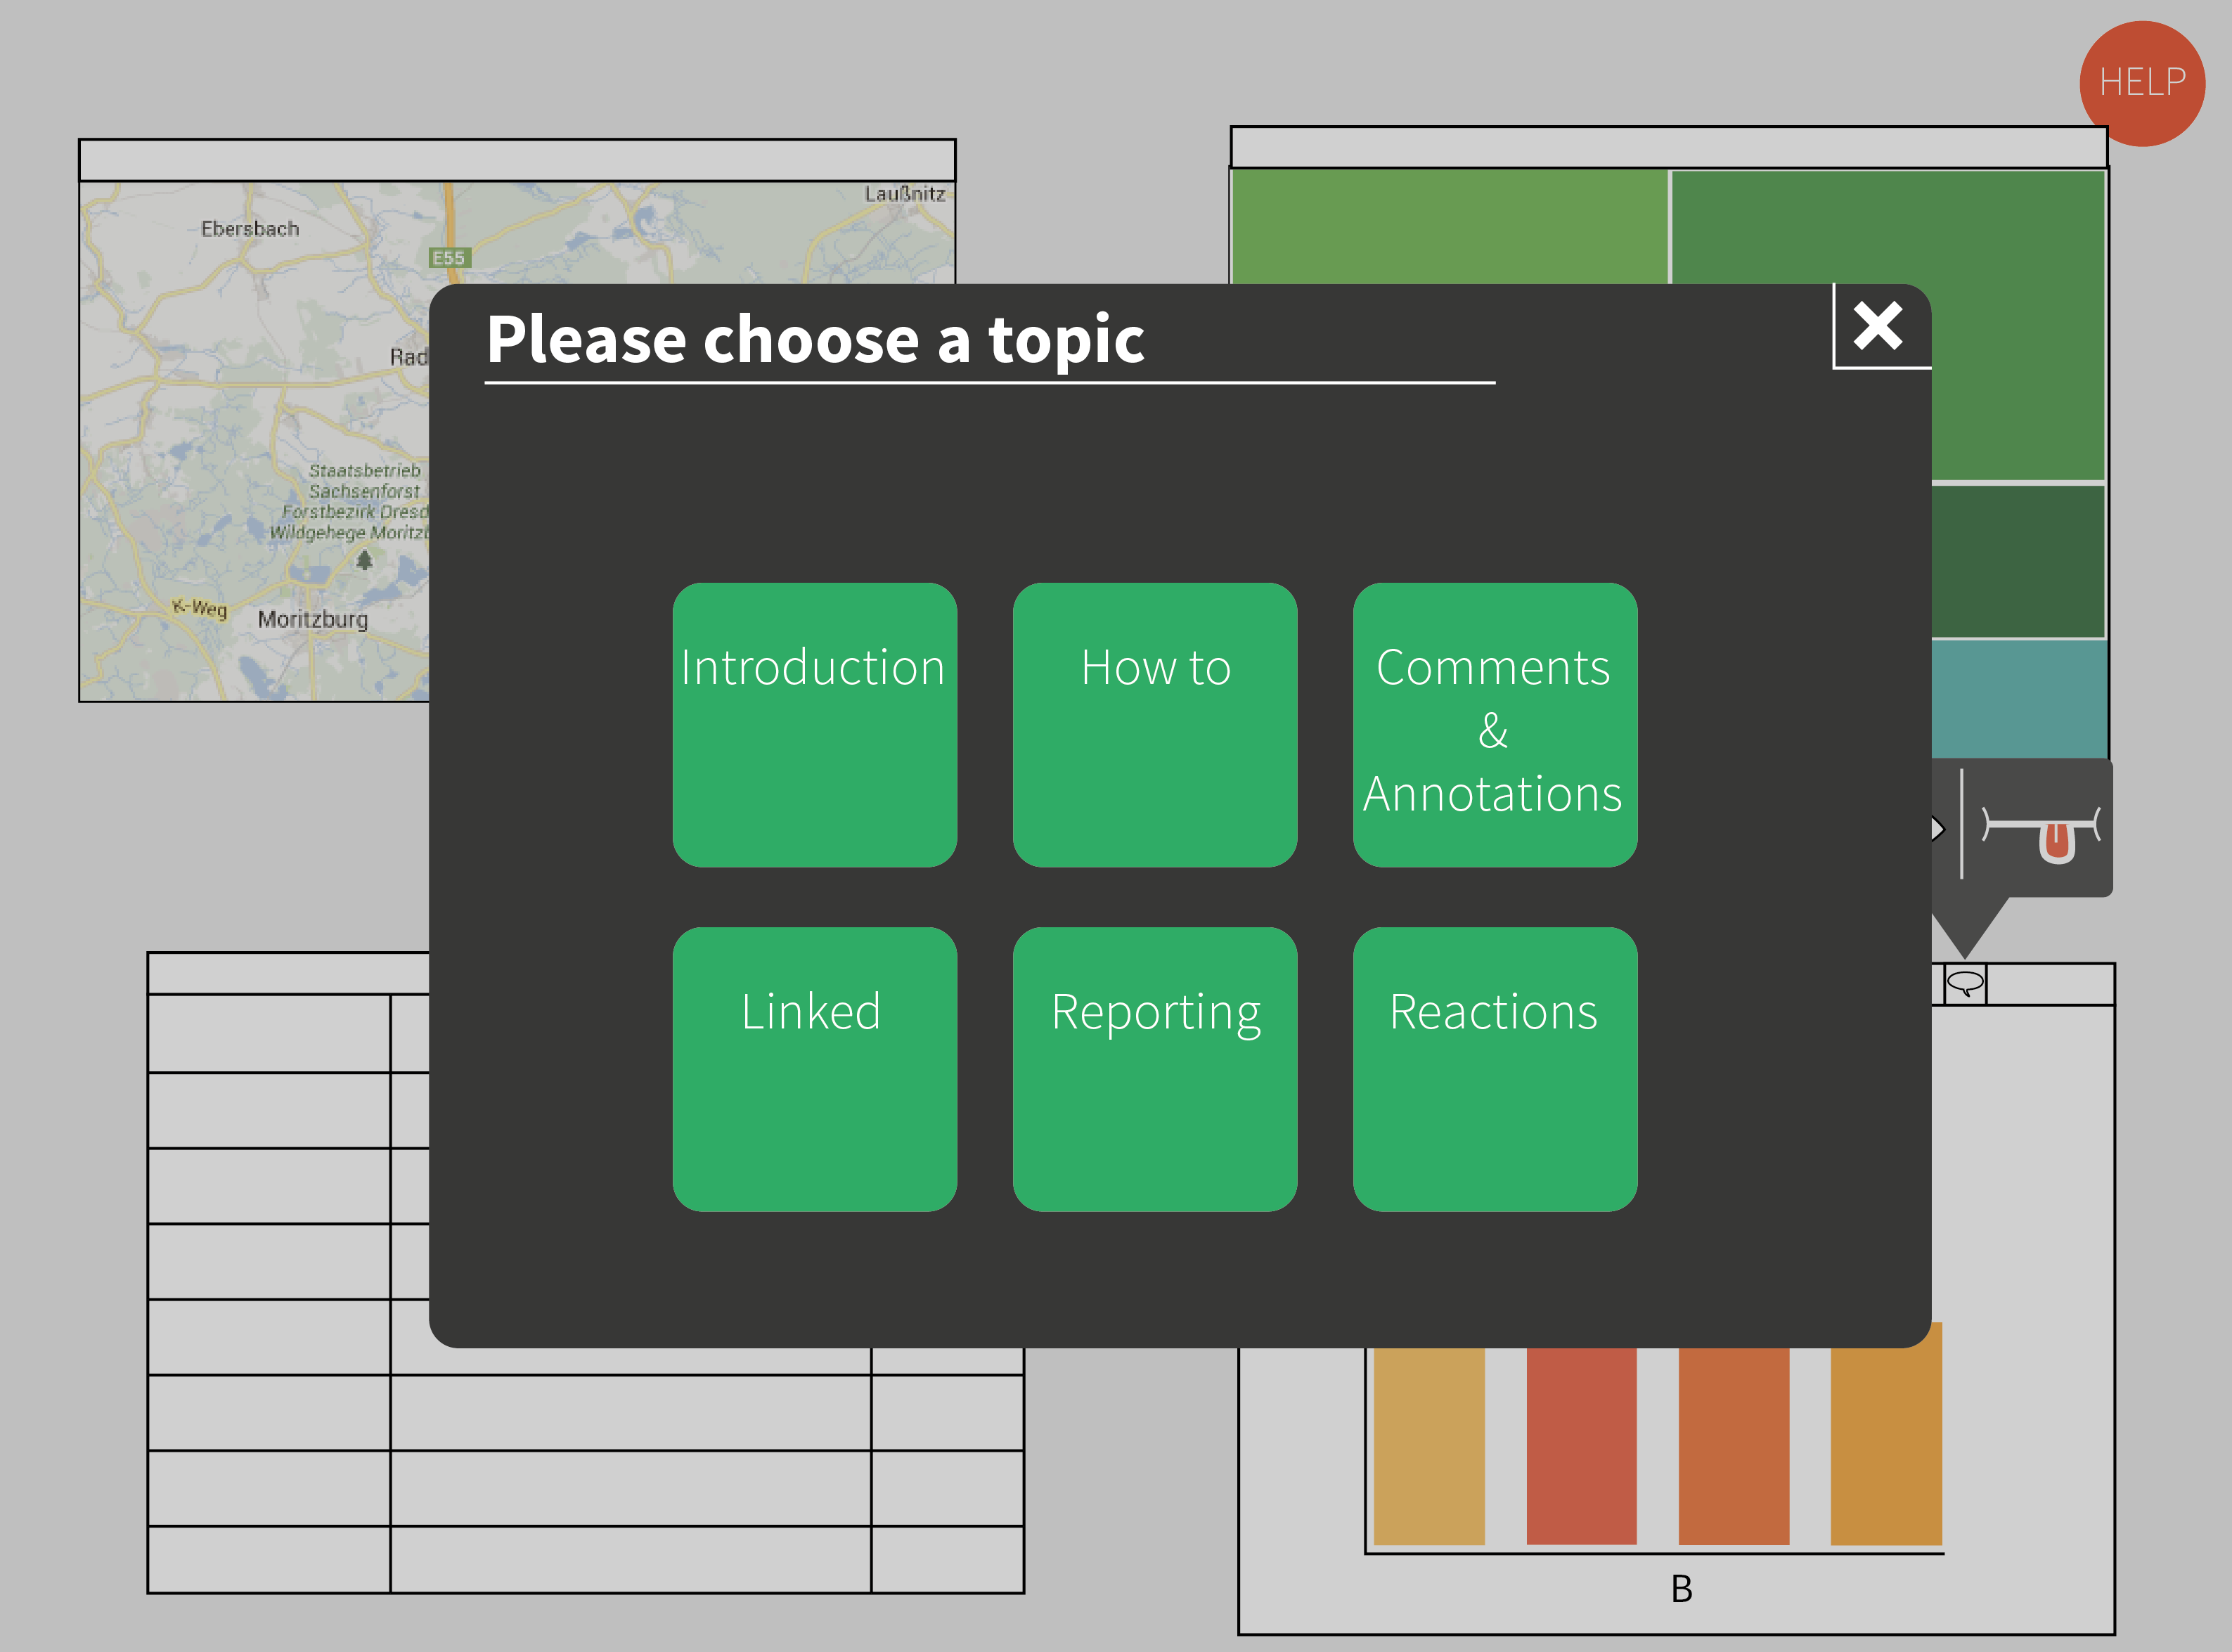
\includegraphics[width=0.5\textwidth]{images/konzeption-meta-step2.png}
   \caption{UI Mockup: Meta-Hilfe}
   \label{figure:meta-step2}
\end{figure}

\section{Synthese}
\label{section:konzeption:synthese}

Für das Konzept wurde das Markup einer Komponente, die Komponentenbeschreibung sowie die API einer Komponente erweitert. In diesem Abschnitt werden die Änderungen zusammengefasst.

\subsubsection{Markup einer Komponente}

\begin{itemize}
	\item CSS Klasse, um Begriffe zur automatischen Verlinkung zu kennzeichnen
	\item CSS Klasse, um Wurzelelement der Visualisierung zu kennzeichnen (Kommentare)
	\item Datenattribut mit URI, um Datenpunkte zu kennzeichnen (Kommentare)
\end{itemize}

\subsubsection{Komponentenbeschreibung}

\begin{itemize}
	\item VISO Konzept der grafischen Repräsentation (Intro)
	\item CSS Selektoren, um UI Elemente für Capabilities zu kennzeichnen (Bedienung)
	\item VISO Operationen, um notwendige Operation auf UI Elementen anzugeben (Bedienung)
	\item Anzahl an Sekunden, die vor einem Screenshot gewartet werden soll (Bedienung)
	\item Text, der Auswirkung der Aktion näher spezifiziert (Bedienung)
	\item Boolean, ob Hilfe für Capability/Operation generiert werden soll oder nicht (Bedienung)
	\item Beispieldaten für Operationen mit Parametern (Bedienung)
	\item Informationen über den zu verwendenden Datensatz (Bedienung)
	\item Ob die Position von Elementen ein visuelles Attribut ist (Kommentare)
	\item Ob die Komponente Datenverarbeitung durchführt (Kommentare)
	\item Ob die Komponente externe Daten anzeigt (Kommentare)
	\item Ob das Layout der Komponente vollständig reproduzierbar ist (Kommentare)
\end{itemize}

\subsubsection{API einer Komponente}

\begin{itemize}
	\item Eine Methode, um Koordinaten in Datenpunkte umzurechnen (Kommentare)
	\item Die Umkehrung der Methode (Datenpunkte $\to$ Koordinaten) (Kommentare)
	\item Eine Methode, um Werte von Attributen eines Datenpunkts zu erhalten (Kommentare)
	\item Zwei Methoden, um ein Memento der Komponente auslesen und wiederherstellen zu können (Kommentare)
\end{itemize}

\subsubsection{VISO}

\begin{itemize}
	\item Beschreibung einer grafischen Repräsentation (Intro)
	\item Link zu Tutorialvideo (Intro)
\end{itemize}

\section{Zusammenfassung}
\label{section:konzeption:zusammenfassung}

\chapter{Implementierung}
\label{chapter:implementierung}

%#####################################################
\printbibliography[title=Literaturverzeichnis]

%\printindex

\end{document}